\documentclass[11pt]{article}

\usepackage[margin=1in]{geometry}
\usepackage{amsmath, amssymb, amsthm}
\usepackage{graphicx}
\usepackage{booktabs}
\usepackage{tikz}
\usetikzlibrary{decorations.pathmorphing, patterns, arrows.meta, calc}
\usepackage[colorlinks=true, linkcolor=blue!50!black, urlcolor=blue!50!black]{hyperref}
\usepackage[expansion=false]{microtype}

\theoremstyle{plain}
\newtheorem{theorem}{Theorem}[section]
\newtheorem{lemma}[theorem]{Lemma}
\newtheorem{proposition}[theorem]{Proposition}
\newtheorem{corollary}[theorem]{Corollary}
\theoremstyle{definition}
\newtheorem{definition}[theorem]{Definition}
\newtheorem{convention}[theorem]{Convention}
\newtheorem{postulate}[theorem]{Postulate}
\newtheorem{example}[theorem]{Example}
\theoremstyle{remark}
\newtheorem{remark}[theorem]{Remark}

\newcommand{\dd}{\mathrm{d}}
\newcommand{\ee}{\mathrm{e}}
\newcommand{\ii}{\mathrm{i}}
\newcommand{\pd}[2]{\frac{\partial #1}{\partial #2}}
\newcommand{\tot}[2]{\frac{\dd #1}{\dd #2}}
\newcommand{\R}{\mathbb{R}}
\newcommand{\vx}{\vec{x}}
\newcommand{\vv}{\vec{v}}
\newcommand{\vp}{\vec{p}}
\newcommand{\vE}{\vec{E}}
\newcommand{\vB}{\vec{B}}

\title{\bfseries From Spacetime to Fields:\\
Special Relativity and Classical Field Theory\\[4pt]
\large From two postulates to the Maxwell Lagrangian}
\author{Lecture notes}
\date{\today}

\begin{document}
\maketitle

\begin{abstract}
\noindent
This document extends the series from mechanics to fields, with every step
of the main logical chain displayed. Part I builds special relativity from
its two postulates: the invariance of the spacetime interval is
\emph{derived}, the Lorentz transformation is obtained from it, and the
kinematic consequences --- relativity of simultaneity, time dilation,
length contraction, velocity composition --- follow with their operational
definitions kept explicit. Minkowski geometry, four-vectors, and the
structure of the Lorentz and Poincar\'e groups are then developed, and the
relativistic particle is treated variationally: the action
$S = -mc\int\dd\tau$ is motivated, its Euler--Lagrange equations solved,
and the four-momentum obtained --- not defined --- as the Noether charge
of spacetime translations, the same theorem of the companion mechanics
notes run on a new symmetry group. Part II passes from particles to
fields: the Lagrangian of the $N$-mass chain is taken to its continuum
limit \emph{at the level of the Lagrangian}, the variational framework of
the mechanics notes is reused verbatim for fields, and the Klein--Gordon
field appears as the simplest Lagrangian consistent with Lorentz
invariance. Noether's theorem for fields localizes conservation laws into
continuity equations and produces the energy-momentum tensor; the
Hamiltonian formulation introduces the field momentum and the canonical
bracket. Part III applies the entire apparatus to electromagnetism: the
field tensor, the gauge-invariant Maxwell Lagrangian, all four Maxwell
equations from variation and from the Bianchi identity, gauge freedom, and
electromagnetic waves. The outlook closes the series: expanded in modes,
every field is a family of harmonic oscillators --- the opening object of
the first document is the atom of field theory. Proofs whose details are
purely technical are placed in appendices; every statement used in the
main text is either proved there or explicitly pointed to its appendix.
\end{abstract}

\clearpage
\tableofcontents
\clearpage

%=======================================================================
\section{Conventions and Notation}
%=======================================================================
\label{sec:conventions}

Dots denote time derivatives. Three-dimensional spatial vectors carry
arrows ($\vx$, $\vv$); their components carry Latin indices $i,j,k$
running over $1,2,3$. Spacetime indices are Greek, $\mu,\nu,\rho,\dots$,
running over $0,1,2,3$, with $x^0 = ct$.

\begin{convention}[Metric signature]\label{conv:signature}
The Minkowski metric is
\begin{equation}
  \eta_{\mu\nu} = \operatorname{diag}(+1,\,-1,\,-1,\,-1),
\end{equation}
the ``mostly-minus'' convention of Schwartz and of Peskin--Schroeder.
Squared timelike intervals are positive.
\end{convention}

\begin{convention}[Summation convention]\label{conv:summation}
\emph{This document breaks with the companion mechanics notes, where all
sums were written out.} From here on, a repeated index --- one upper, one
lower --- is summed over its range:
\begin{equation}
  a^\mu b_\mu \;\equiv\; \sum_{\mu=0}^{3} a^\mu b_\mu
  = a^0 b_0 + a^1 b_1 + a^2 b_2 + a^3 b_3 .
\end{equation}
An index appearing twice is a \emph{dummy} index and may be renamed
freely; an index appearing once must appear, with the same placement, on
both sides of every equation. Field-theory formulas become impractically long without this
convention; the cost is vigilance about index placement, and the reader
should expand a few contractions by hand early on until the shorthand is
trusted.
\end{convention}

\begin{convention}[Units]\label{conv:units}
Sections~\ref{sec:postulates}--\ref{sec:minkowski} keep the speed of
light $c$ explicit: while the four-dimensional formalism is being
assembled, $c$ is the conversion factor between meters and seconds, and
tracking it is a dimension check on every line. At the end of
\S\ref{sec:minkowski} we set $c=1$ once and for all; the lost factors are
recoverable uniquely by dimensional analysis.
\end{convention}

\noindent
The recurring symbols are collected here for reference; each is
re-introduced where it first appears.

\begin{center}
\begin{tabular}{llll}
\toprule
Symbol & Definition & First appears & Meaning \\
\midrule
$\beta$ & $\beta = v/c$ & \S\ref{sec:postulates} & dimensionless velocity \\
$\gamma$ & $\gamma = (1-\beta^2)^{-1/2}$ & \S\ref{sec:postulates} & Lorentz factor \\
$\phi$ & $\tanh\phi = \beta$ & \S\ref{sec:postulates} & rapidity \\
$s^2$ & $s^2 = c^2 t^2 - |\vx|^2$ & \S\ref{sec:postulates} & spacetime interval \\
$\eta_{\mu\nu}$ & $\operatorname{diag}(+,-,-,-)$ & \S\ref{sec:minkowski} & Minkowski metric \\
$\Lambda^\mu{}_\nu$ & $\eta_{\mu\nu}\Lambda^\mu{}_\rho\Lambda^\nu{}_\sigma = \eta_{\rho\sigma}$ & \S\ref{sec:minkowski} & Lorentz transformation \\
$\tau$ & $c^2\dd\tau^2 = \dd x^\mu \dd x_\mu$ & \S\ref{sec:minkowski} & proper time \\
$\partial_\mu$ & $\partial/\partial x^\mu$ & \S\ref{sec:minkowski} & spacetime gradient \\
$\Box$ & $\Box = \partial_\mu\partial^\mu$ & \S\ref{sec:minkowski} & d'Alembertian \\
$\phi(x)$ & --- & \S\ref{sec:chain-to-field} & scalar field (context separates it from rapidity) \\
$\pi(x)$ & $\pi = \partial\mathcal L/\partial\dot\phi$ & \S\ref{sec:hamiltonian-fields} & field momentum density \\
$F_{\mu\nu}$ & $\partial_\mu A_\nu - \partial_\nu A_\mu$ & \S\ref{sec:field-tensor} & electromagnetic field tensor \\
\bottomrule
\end{tabular}
\end{center}

\vspace{1ex}
\noindent
Cross-references to the companion documents are written as
[Mech.\ \S$n$] for the variational mechanics course and [Osc.\ \S$n$] for
the oscillator reference.

%=======================================================================
\clearpage
\part{Spacetime}
%=======================================================================

%=======================================================================
\section{The Two Postulates and the Lorentz Transformation}
%=======================================================================
\label{sec:postulates}

\subsection{A wave equation with a problem}
\label{sec:wave-problem}

The oscillator reference ended with the wave equation [Osc.\ \S9]: the
continuum limit of a chain of masses is a displacement field $u(x,t)$
obeying
\begin{equation}
  \pd{^2 u}{t^2} = c_s^2\, \pd{^2 u}{x^2},
  \qquad c_s^2 = \frac{T}{\mu},
  \label{eq:wave-eq}
\end{equation}
with $T$ the tension and $\mu$ the mass per length. Newtonian mechanics
comes with a democracy of inertial frames: the laws take the same form
for every observer in uniform motion, frames being related by the
\emph{Galilean transformation}
\begin{equation}
  \bar x = x - vt, \qquad \bar t = t .
  \label{eq:galilean}
\end{equation}
Is the wave equation a law in this sense? Chain rule: for
$u(x,t) = \bar u(\bar x,\bar t)$,
\begin{equation}
  \pd{}{x} = \pd{}{\bar x},
  \qquad
  \pd{}{t} = \pd{}{\bar t} - v\,\pd{}{\bar x},
\end{equation}
so that
\begin{equation}
  \pd{^2 u}{t^2} - c_s^2 \pd{^2 u}{x^2}
  \;=\;
  \pd{^2 \bar u}{\bar t^2}
  \;-\; 2v\,\frac{\partial^2 \bar u}{\partial\bar x\,\partial\bar t}
  \;+\; \bigl(v^2 - c_s^2\bigr)\pd{^2 \bar u}{\bar x^2}.
  \label{eq:wave-not-invariant}
\end{equation}
The right-hand side is \emph{not} of the form
$\bar u_{\bar t\bar t} - c_s^2\,\bar u_{\bar x\bar x}$: the wave equation
changes form under a Galilean boost. For sound this is not a problem --- the
equation was derived in the rest frame of the \emph{medium}, and the
medium's rest frame is genuinely special. A moving observer measures
different sound speeds upstream and downstream, and
Eq.~\eqref{eq:wave-not-invariant} is precisely the equation that says so.

The problem arrives with light. Maxwell's equations predict
electromagnetic waves of speed
$c = (\mu_0\varepsilon_0)^{-1/2} \approx 3.00\times 10^8\,\mathrm{m/s}$
--- a wave equation of the form \eqref{eq:wave-eq} with $c_s \to c$, as
Part III will derive. By the logic above, that equation should hold only
in the rest frame of light's medium, and measuring the anisotropy of the
speed of light should reveal the Earth's motion through it. The
Michelson--Morley experiment (1887) and its successors looked and found
nothing: the speed of light is the same in every direction, in every
season, to (by now) parts in $10^{17}$. [experimental input; we take it
as given.]

Einstein's move (1905) was to stop treating the null result as a
conspiracy to be explained and promote it to a law of nature. Two
postulates:

\begin{postulate}[Relativity]\label{post:relativity}
The laws of physics take the same form in every inertial frame. No
experiment performed inside a laboratory can detect the laboratory's
uniform motion.
\end{postulate}

\begin{postulate}[Invariance of the speed of light]\label{post:light}
There is a finite speed $c$ that is the same in every inertial frame,
independent of the motion of the source. Light in vacuum travels at $c$.
\end{postulate}

\noindent
Postulate~\ref{post:relativity} simply retains Galileo's principle. What is abandoned is
the Galilean transformation \eqref{eq:galilean} --- because, as
Eq.~\eqref{eq:wave-not-invariant} shows, it is \emph{incompatible} with
Postulate~\ref{post:light}: under \eqref{eq:galilean} a speed-$c$ signal
in one frame has speed $c \pm v$ in another. The task of this section is
to find the transformation law that the two postulates force, and the
strategy is to first find what the postulates leave \emph{invariant}.

\subsection{Setup: events, frames, and the standard configuration}
\label{sec:setup}

An \emph{event} is a point of spacetime: something with a where and a
when, idealized to a point --- a firecracker, the coincidence of two
particles, one tick of one clock. An inertial frame $S$ assigns
coordinates $(t, x, y, z)$ to every event, operationally by a lattice of
rulers and synchronized clocks at rest in $S$; we write the time
coordinate as $x^0 = ct$ so that all four coordinates carry the same
dimension.

Two frames $S$ and $S'$ are in \emph{standard configuration} if their
axes are parallel, $S'$ moves with velocity $v$ along the common
$x$-axis, and the origins coincide: the event $(0,0,0,0)$ has these
coordinates in both frames. For the rest of this section we suppress the
transverse coordinates $y, z$ and work in the $(ct, x)$ plane; the
transverse directions are dealt with in Appendix~\ref{app:linearity}
(they turn out to be spectators: $y' = y$, $z' = z$).

Two facts about the transformation
$(ct, x) \mapsto (ct', x')$ come before the postulates proper:

\begin{lemma}[Linearity]\label{lem:linearity}
The transformation between two inertial frames in standard configuration
is linear:
\begin{equation}
  \begin{pmatrix} ct' \\ x' \end{pmatrix}
  = \mathsf{\Lambda}
  \begin{pmatrix} ct \\ x \end{pmatrix}
\end{equation}
for a constant matrix $\mathsf{\Lambda}$ depending only on $v$.
\end{lemma}

\noindent
The physics behind the lemma is the homogeneity of space and time ---
no event is privileged, so coordinate \emph{differences} must transform
the same way wherever they sit --- plus continuity. The full argument is
technical and lives in Appendix~\ref{app:linearity}. [stated; proved in
Appendix~\ref{app:linearity}.]

\subsection{The invariant: derivation of the interval}
\label{sec:interval}

Define, for any pair of events with separations $\Delta t$, $\Delta x$ in
the frame $S$, the \emph{interval}
\begin{equation}
  \Delta s^2 \;=\; c^2\,\Delta t^2 - \Delta x^2 .
  \label{eq:interval-def}
\end{equation}
(No claim yet that this is a good idea; the definition is justified by
Theorem~\ref{thm:interval} immediately below.) Since the transformation is linear,
separations transform like coordinates, and it suffices to study
$s^2 = c^2t^2 - x^2$ for events relative to the common origin.

\begin{theorem}[Invariance of the interval]\label{thm:interval}
For any two inertial frames in standard configuration and any pair of
events,
\begin{equation}
  \boxed{\;
  c^2\,\Delta t'^2 - \Delta x'^2 \;=\; c^2\,\Delta t^2 - \Delta x^2 .
  \;}
  \label{eq:interval-invariance}
\end{equation}
\end{theorem}

\begin{proof}
The proof runs in three steps: the postulates first pin down the
\emph{zero set} of $s^2$, then its scale, and isotropy kills the scale.

\emph{Step 1: null separations are preserved.} Introduce the null
coordinates
\begin{equation}
  u = ct - x, \qquad w = ct + x,
  \qquad\text{so that}\qquad
  s^2 = u\,w .
  \label{eq:null-coords}
\end{equation}
A pair of events with $u = 0$ (i.e.\ $x = ct$) can be connected by a
light signal moving in the $+x$ direction; a pair with $w = 0$, by one
moving in the $-x$ direction. Postulate~\ref{post:light} says light moves
at $c$ in $S'$ as well: therefore $u = 0 \Rightarrow u' = 0$ and
$w = 0 \Rightarrow w' = 0$. (The boost does not swap the two light rays:
at $v = 0$ the transformation is the identity, and by continuity in $v$
the rightward ray cannot jump onto the leftward one.)

\emph{Step 2: the interval can change at most by an overall factor.}
In the null coordinates the linear transformation reads
$u' = \alpha u + \beta_1 w$, $w' = \beta_2 u + \delta w$. Step 1 forces
$\beta_1 = \beta_2 = 0$ (set $u=0$, vary $w$, demand $u'=0$; and
conversely). Hence
\begin{equation}
  u' = \alpha(v)\, u, \qquad w' = \delta(v)\, w,
  \qquad\Longrightarrow\qquad
  s'^2 = u'w' = \alpha(v)\,\delta(v)\; s^2
  \;\equiv\; \lambda(v)\, s^2 ,
  \label{eq:scale-factor}
\end{equation}
with $\alpha, \delta > 0$ for a transformation continuously connected to
the identity that does not reverse the direction of time. The whole
quadratic form is rescaled by a single velocity-dependent number
$\lambda(v) > 0$.

\emph{Step 3: isotropy forces $\lambda = 1$.} Two properties of
$\lambda$:
\begin{itemize}
  \item \textbf{Reciprocity.} The inverse transformation, from $S'$ back
  to $S$, is the boost with velocity $-v$
  (Postulate~\ref{post:relativity}: $S$ moves at $-v$ as seen from $S'$,
  and neither frame is privileged). Applying \eqref{eq:scale-factor}
  twice, $s^2 = \lambda(-v)\,s'^2 = \lambda(-v)\lambda(v)\,s^2$, so
  \begin{equation}
    \lambda(v)\,\lambda(-v) = 1 .
  \end{equation}
  \item \textbf{Isotropy.} Space has no preferred direction: the physics
  of a boost to the right at speed $|v|$ is the mirror image of a boost
  to the left. Formally, let $P: (ct, x) \mapsto (ct, -x)$; then the
  boost of velocity $-v$ is $P\,\Lambda_v\,P$. Since $P$ leaves $s^2$
  unchanged, the scale factors of $\Lambda_{-v}$ and $\Lambda_v$ are
  equal:
  \begin{equation}
    \lambda(-v) = \lambda(v) .
  \end{equation}
\end{itemize}
Together, $\lambda(v)^2 = 1$; positivity gives $\lambda(v) = 1$.
\end{proof}

\begin{remark}[What just happened]
Postulate~\ref{post:light} by itself only protects the light cone
$s^2 = 0$; it is Postulate~\ref{post:relativity} --- entering through
reciprocity and isotropy --- that rigidifies the whole quadratic form.
The interval \eqref{eq:interval-def} is the replacement for the two
quantities Newtonian physics held absolute separately: the time between
two events and the distance between them are now frame-dependent, and
only the combination $c^2\Delta t^2 - \Delta x^2$ is common property.
Figure~\ref{fig:hyperbolae} shows the geometry: the events at fixed
interval from the origin form hyperbolae, and every inertial frame's unit
ticks lie on the \emph{same} hyperbolae.
\end{remark}

\begin{figure}[htbp]
  \centering
  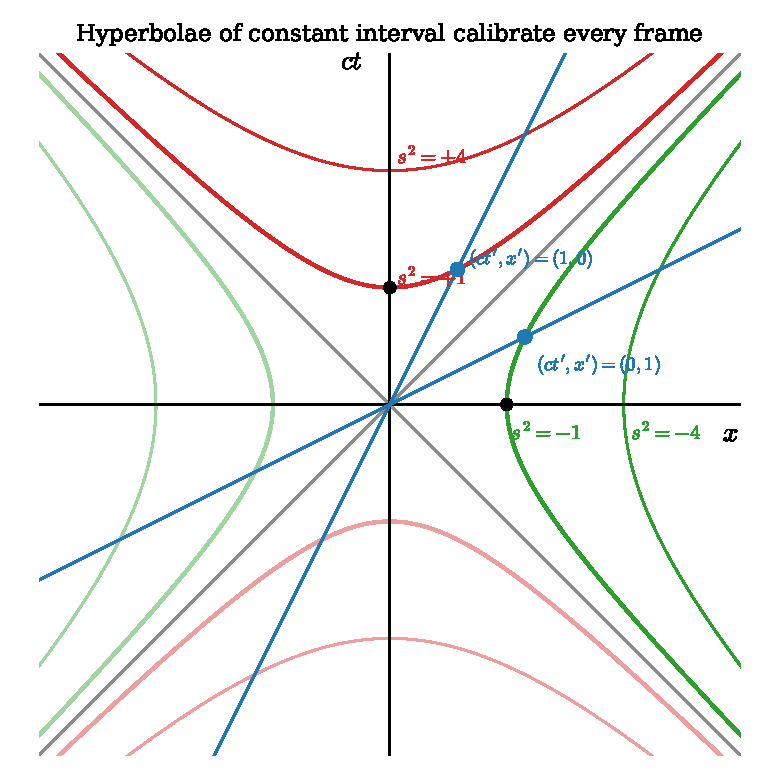
\includegraphics[width=0.62\textwidth]{fig_interval_hyperbolae.pdf}
  \caption{Curves of constant interval $s^2 = c^2t^2 - x^2$ (timelike in
  red, spacelike in green) and the axes of a boosted frame
  ($\beta = 0.5$, blue). The boosted frame's unit events --- one tick of
  its clock at its origin, one meter along its ruler at its zero time ---
  lie on the same unit hyperbolae as the unprimed frame's. The hyperbolae
  are drawn from the exact equations $ct = \pm\sqrt{s^2 + x^2}$ and
  $x = \pm\sqrt{s^2 + (ct)^2}$.}
  \label{fig:hyperbolae}
\end{figure}

\subsection{Two routes from the invariant to the transformation}
\label{sec:lorentz-derivation}

Theorem~\ref{thm:interval} converts the search for the transformation law
into a purely algebraic problem: \emph{find all linear maps of the
$(ct,x)$ plane that preserve $c^2t^2 - x^2$}, then pick out the one that
describes a boost of velocity $v$. In the spirit of the companion notes'
double derivation of Hamilton's equations [Mech.\ \S6.2], we solve it
twice: once in coordinates adapted to the problem's structure, where the
answer explains itself, and once by brute force in the physical
coordinates, where every coefficient is worked out by hand.

\paragraph{Route 1: null coordinates.}
The work is already done. Any linear map that preserves
$s^2 = uw$ in particular preserves its zero set, the two null lines, so
Steps 1--2 of the proof of Theorem~\ref{thm:interval} apply verbatim:
in the null coordinates \eqref{eq:null-coords} the map must have the
diagonal form $u' = \alpha u$, $w' = \delta w$ with $\alpha, \delta > 0$
--- and now, since the interval is preserved exactly,
\begin{equation}
  \alpha\,\delta = \lambda = 1,
  \qquad\text{i.e.}\qquad
  \delta = \frac{1}{\alpha}.
\end{equation}
One free positive number $\alpha$ remains. Since the exponential is a
bijection from $\R$ onto the positive reals, we may write
$\alpha = \ee^{\phi}$ for a unique $\phi \in \R$ --- pure repackaging,
$\phi = \ln\alpha$, but repackaging with a payoff: composing two such
maps \emph{multiplies} the $\alpha$'s, hence \emph{adds} the $\phi$'s, so
the parameter $\phi$ is the one in which the group law will look
simplest (used in \S\ref{sec:composition}). The one-parameter
family is
\begin{equation}
  u' = \ee^{\phi}\, u,
  \qquad
  w' = \ee^{-\phi}\, w,
  \qquad \phi \in \R :
  \label{eq:null-boost}
\end{equation}
each null coordinate is stretched by exactly the factor that shrinks the
other, and the product $uw$ survives.

Now translate back. Inverting \eqref{eq:null-coords},
$ct = \tfrac12(w+u)$ and $x = \tfrac12(w-u)$, and the same relations hold
in the primed frame. Substitute \eqref{eq:null-boost}, then
$u = ct - x$, $w = ct + x$:
\begin{align}
  ct' = \tfrac12\bigl(w' + u'\bigr)
      &= \tfrac12\bigl(\ee^{-\phi}(ct + x) + \ee^{\phi}(ct - x)\bigr)
      \notag\\
      &= ct\,\frac{\ee^{\phi} + \ee^{-\phi}}{2}
       - x\,\frac{\ee^{\phi} - \ee^{-\phi}}{2}
       \;=\; ct\,\cosh\phi - x\,\sinh\phi,
  \notag\\[2pt]
  x'  = \tfrac12\bigl(w' - u'\bigr)
      &= \tfrac12\bigl(\ee^{-\phi}(ct + x) - \ee^{\phi}(ct - x)\bigr)
      \notag\\
      &= -\,ct\,\frac{\ee^{\phi} - \ee^{-\phi}}{2}
       + x\,\frac{\ee^{\phi} + \ee^{-\phi}}{2}
       \;=\; -\,ct\,\sinh\phi + x\,\cosh\phi ,
  \label{eq:hyperbolic-rotation}
\end{align}
where the last step in each line is nothing but the definitions
$\cosh\phi = \tfrac12(\ee^{\phi} + \ee^{-\phi})$,
$\sinh\phi = \tfrac12(\ee^{\phi} - \ee^{-\phi})$: the hyperbolic
functions are not imported; they arise directly as the symmetric and
antisymmetric combinations of the two exponential stretch factors.

\begin{remark}[Why hyperbolic functions were inevitable]
\label{rem:hyperbolic-geometry}
Compare with the Euclidean plane, feature by feature:
\begin{center}
\begin{tabular}{lcc}
\toprule
 & rotation & boost \\
\midrule
preserved form & $x^2 + y^2$ \ (circles) & $c^2t^2 - x^2$ \ (hyperbolae) \\[2pt]
matrix &
$\begin{pmatrix} \cos\theta & -\sin\theta \\ \sin\theta & \cos\theta \end{pmatrix}$ &
$\begin{pmatrix} \cosh\phi & -\sinh\phi \\ -\sinh\phi & \cosh\phi \end{pmatrix}$ \\[10pt]
parameter & angle $\theta$, additive & rapidity $\phi$, additive \\[2pt]
level-set parametrization & $(\cos\theta, \sin\theta)$ & $(\cosh\phi, \sinh\phi)$ \\[2pt]
function family & trigonometric & hyperbolic \\[2pt]
eigenvalues & $\ee^{\pm\ii\theta}$ \ (complex) & $\ee^{\pm\phi}$ \ (real; Remark~\ref{rem:eigen}) \\
\bottomrule
\end{tabular}
\end{center}
A rotation slides points along the circles that its invariant form
draws; Eq.~\eqref{eq:hyperbolic-rotation} slides events along the
hyperbolae of Fig.~\ref{fig:hyperbolae}, which its invariant form draws
--- a \emph{hyperbolic rotation}, with
$\cosh^2\phi - \sinh^2\phi = 1$ playing the role of
$\cos^2\theta + \sin^2\theta = 1$. Every row of the table follows from
the single sign difference in the preserved form, and the last row ---
real eigenvalues where rotations have complex ones --- is the difference
with the most physical content, as Remark~\ref{rem:eigen} will show.
\end{remark}

It remains to identify the parameter $\phi$, called the
\emph{rapidity}, in terms of the velocity. The origin of $S'$ is the
worldline $x' = 0$; by \eqref{eq:hyperbolic-rotation} that is the line
$x = ct\,\tanh\phi$. But the origin of $S'$ moves at velocity $v$ by
definition of the standard configuration, i.e.\ along $x = vt$. Hence
\begin{equation}
  \boxed{\;
  \tanh\phi = \frac{v}{c} \equiv \beta,
  \qquad
  \cosh\phi = \frac{1}{\sqrt{1-\beta^2}} \equiv \gamma,
  \qquad
  \sinh\phi = \gamma\beta .
  \;}
  \label{eq:rapidity-def}
\end{equation}
(The last two follow from the first and $\cosh^2 - \sinh^2 = 1$.)
Substituting into \eqref{eq:hyperbolic-rotation} gives the boxed result
of Theorem~\ref{thm:lorentz} below.

\paragraph{Route 2: undetermined coefficients.}
Now the same problem with no change of variables: write the general
linear map in the physical coordinates and let the invariant grind out
the coefficients.

\emph{(1) Ansatz.} By Lemma~\ref{lem:linearity},
\begin{equation}
  ct' = A\,ct + B\,x,
  \qquad
  x' = D\,ct + E\,x,
\end{equation}
with four constants depending on $\beta$ only.

\emph{(2) Motion of the moving origin.} The worldline $x' = 0$ is, by
definition of the standard configuration, the line $x = \beta\,ct$.
Substituting: $0 = D\,ct + E\beta\,ct$ for all $t$, so $D = -\beta E$
and
\begin{equation}
  x' = E\,(x - \beta\,ct).
\end{equation}
One coefficient down, three to go.

\emph{(3) Balance the invariant.} Demand
$(ct')^2 - x'^2 = (ct)^2 - x^2$ \emph{identically} in $(ct, x)$. Expand
the left side,
\begin{equation}
  (A\,ct + B x)^2 - E^2(x - \beta\,ct)^2,
\end{equation}
and match the coefficients of $(ct)^2$, $x^2$, and the cross term
$(ct)\,x$ separately --- an identity between quadratic forms is three
scalar equations:
\begin{alignat}{2}
  A^2 - \beta^2 E^2 &= 1
  &\qquad&\text{[$(ct)^2$ term]}
  \notag\\
  B^2 - E^2 &= -1
  &&\text{[$x^2$ term]}
  \label{eq:balance}\\
  AB + \beta E^2 &= 0
  &&\text{[$(ct)\,x$ term]}
  \notag
\end{alignat}

\emph{(4) Solve.} Square the third equation, $A^2 B^2 = \beta^2 E^4$,
and substitute the first two in the forms $A^2 = 1 + \beta^2 E^2$ and
$B^2 = E^2 - 1$:
\begin{equation}
  (1 + \beta^2 E^2)(E^2 - 1) = \beta^2 E^4
  \quad\Longrightarrow\quad
  E^2 - 1 - \beta^2 E^2 = 0
  \quad\Longrightarrow\quad
  E^2 = \frac{1}{1 - \beta^2}.
\end{equation}
So $E = \gamma$, and back-substituting,
\begin{equation}
  A^2 = 1 + \beta^2\gamma^2 = (1 - \beta^2)\gamma^2 + \beta^2\gamma^2
      = \gamma^2
  \;\Rightarrow\; A = \gamma,
  \qquad
  B = -\frac{\beta E^2}{A} = -\gamma\beta .
\end{equation}
The signs: the equations \eqref{eq:balance} are quadratic and admit sign
flips of $(A, B)$ and of $E$; the positive roots are selected by
continuity to the identity at $\beta = 0$, the other choices being
spatial reflection and/or time reversal, excluded by the standard
configuration. The result is $ct' = \gamma(ct - \beta x)$,
$x' = \gamma(x - \beta ct)$ --- the two routes meet.

\begin{remark}[What the change of coordinates achieved]
\label{rem:two-routes}
Route 2 is three coupled quadratic equations and an elimination; Route 1
is two decoupled one-line equations, \eqref{eq:null-boost}. The
difference is entirely in the coordinates: the null variables $u, w$ are
adapted to the preserved form ($s^2 = uw$ has no diagonal terms to
balance), and in them the transformation is diagonal. This is the same
simplification that normal coordinates achieve for coupled oscillators [Osc.\
\S6]: pick the variables the structure prefers, and the coupled system
falls apart. Remark~\ref{rem:eigen} will name the sense in which the
null coordinates are exactly the ``normal coordinates'' of a boost.
\end{remark}

\noindent
Collecting the result of both routes:

\begin{theorem}[Lorentz transformation]\label{thm:lorentz}
Two inertial frames in standard configuration with relative velocity
$v = \beta c$, $|\beta| < 1$, are related by
\begin{equation}
  \boxed{\;
  ct' = \gamma\,(ct - \beta x),
  \qquad
  x' = \gamma\,(x - \beta\, ct),
  \qquad
  \gamma = \frac{1}{\sqrt{1-\beta^2}},
  \;}
  \label{eq:lorentz}
\end{equation}
equivalently by the rapidity form \eqref{eq:hyperbolic-rotation} with
$\tanh\phi = \beta$. The inverse transformation is the same formula with
$\beta \to -\beta$.
\end{theorem}

\begin{remark}[Sanity checks]\label{rem:sanity}
(i) \emph{Nonrelativistic limit.} For $\beta \ll 1$,
$\gamma = 1 + \tfrac12\beta^2 + O(\beta^4)$, and \eqref{eq:lorentz}
becomes $x' = x - vt + O(\beta^2)$, $t' = t - vx/c^2 + O(\beta^2)$: the
Galilean transformation is recovered in the regime where it was ever
tested, with the first correction hitting the \emph{time} coordinate ---
the term $vx/c^2$ is the relativity of simultaneity, previewed.
(ii) \emph{Light stays light.} If $x = ct$ then
$x' = \gamma(ct - \beta ct) = ct'$, as built in.
(iii) \emph{The speed limit.} $\gamma$ is real only for $|\beta| < 1$:
no inertial frame moves at or above $c$ relative to another. Rapidity
makes the limit natural --- $\phi$ ranges over all of $\R$ while
$\beta = \tanh\phi$ is confined to $(-1, 1)$.
\end{remark}

\subsection{Composition: the group structure and velocity addition}
\label{sec:composition}

What happens when boosts are stacked --- a passenger walking in a moving
train? Compose two transformations of the form
\eqref{eq:hyperbolic-rotation} with rapidities $\phi_1$, $\phi_2$. The
matrices are
\begin{equation}
  \mathsf{\Lambda}(\phi) =
  \begin{pmatrix} \cosh\phi & -\sinh\phi \\ -\sinh\phi & \cosh\phi \end{pmatrix},
\end{equation}
and the hyperbolic addition formulas
$\cosh(\phi_1{+}\phi_2) = \cosh\phi_1\cosh\phi_2 + \sinh\phi_1\sinh\phi_2$,
$\sinh(\phi_1{+}\phi_2) = \sinh\phi_1\cosh\phi_2 + \cosh\phi_1\sinh\phi_2$
give, by direct multiplication,
\begin{equation}
  \boxed{\;
  \mathsf{\Lambda}(\phi_2)\,\mathsf{\Lambda}(\phi_1)
  = \mathsf{\Lambda}(\phi_1 + \phi_2)
  \;}
  \label{eq:rapidity-addition}
\end{equation}
--- boosts along a common axis form a one-parameter group, and
\emph{rapidities simply add}, exactly as rotation angles add in the
plane. Velocities do not:

\begin{corollary}[Velocity composition]\label{cor:velocity-addition}
If $S'$ moves at $\beta_1$ relative to $S$, and a body moves at
$\beta_2$ relative to $S'$ (both along $x$), its velocity relative to
$S$ is
\begin{equation}
  \boxed{\;
  \beta_{12} = \tanh(\phi_1 + \phi_2)
  = \frac{\beta_1 + \beta_2}{1 + \beta_1\beta_2}.
  \;}
  \label{eq:velocity-addition}
\end{equation}
\end{corollary}

\begin{proof}
Immediate from \eqref{eq:rapidity-addition} and the addition formula for
$\tanh$.
\end{proof}

\noindent
The denominator does the work: for $\beta_1, \beta_2 \in (0,1)$ it
exceeds $1$ just enough to keep $\beta_{12} < 1$, and if either input is
$1$ the output is $1$ --- light composed with anything is light.
Figure~\ref{fig:rapidity} composes eight successive boosts of
$\beta = 0.5$: the Galilean sum crosses the light speed on the second
step; the true velocity approaches it and never arrives, while the
rapidity grows linearly.

\begin{figure}[htbp]
  \centering
  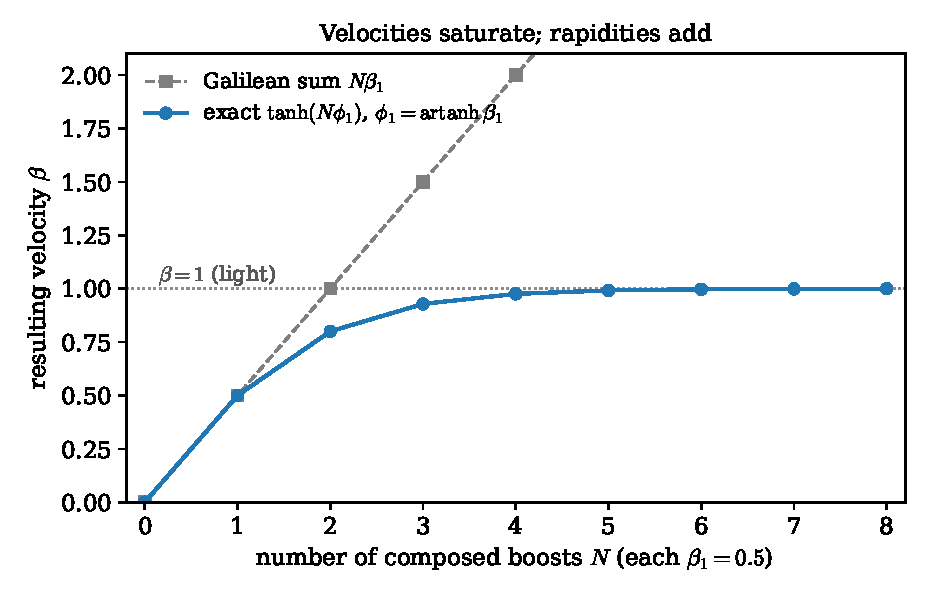
\includegraphics[width=0.75\textwidth]{fig_rapidity_addition.pdf}
  \caption{Composing $N$ successive boosts of $\beta_1 = 0.5$. Gray
  squares: the Galilean prediction $N\beta_1$. Blue circles: the exact
  result $\tanh(N\phi_1)$ with $\phi_1 = \operatorname{artanh}(0.5)$,
  from Eq.~\eqref{eq:rapidity-addition}.}
  \label{fig:rapidity}
\end{figure}

\begin{remark}[The light cone is an eigendirection]\label{rem:eigen}
Equation~\eqref{eq:null-boost} was secretly an eigendecomposition.
The characteristic polynomial of $\mathsf{\Lambda}(\phi)$ is
\begin{equation}
  \det\bigl(\mathsf{\Lambda}(\phi) - \lambda\,\mathsf{1}\bigr)
  = (\cosh\phi - \lambda)^2 - \sinh^2\phi
  = \lambda^2 - 2\lambda\cosh\phi + 1,
\end{equation}
with roots
\begin{equation}
  \lambda_\pm = \cosh\phi \pm \sinh\phi = \ee^{\pm\phi} :
\end{equation}
real, positive, and reciprocal. The eigenvectors are the null
directions: $(ct, x) \propto (1, -1)$, the line $w = 0$, carries
$\lambda = \ee^{\phi}$, and $(1, 1)$, the line $u = 0$, carries
$\lambda = \ee^{-\phi}$ --- \emph{the eigenvectors of a boost are the
light cone}. The null coordinates of Route 1 are the eigencoordinates,
Eq.~\eqref{eq:null-boost} is the diagonalized boost, and the geometric
action is now plain: stretch one light-ray direction by $\ee^{\phi}$,
compress the other by $\ee^{-\phi}$, with
$\det = \ee^{\phi}\ee^{-\phi} = 1$ --- an area-preserving
\emph{squeeze} of the plane, sliding every event along its invariant
hyperbola (Fig.~\ref{fig:hyperbolae}) while the asymptotes stay put.
Three payoffs:
\begin{itemize}
  \item \textbf{Postulate~\ref{post:light}, restated in linear
  algebra.} The light cone is the common eigendirection of every boost
  --- the directions of spacetime on which all inertial observers
  agree. ``The speed of light is invariant'' and ``light rays are
  eigenvectors'' are the same sentence in two languages.
  \item \textbf{Composition, in one line.} Composing boosts multiplies
  eigenvalues on shared eigenvectors:
  $\ee^{\phi_1}\ee^{\phi_2} = \ee^{\phi_1 + \phi_2}$, which is
  Eq.~\eqref{eq:rapidity-addition} again --- rapidity addition is the
  multiplicativity of eigenvalues, read on the light cone.
  \item \textbf{The eigenvalue is physical.} The stretch factor
  \begin{equation}
    \ee^{\phi} = \cosh\phi + \sinh\phi = \gamma(1 + \beta)
    = \sqrt{\frac{1+\beta}{1-\beta}}
  \end{equation}
  will return: it is the relativistic Doppler factor, the
  ratio by which a receding observer sees periods stretched, derived as
  such in \S\ref{sec:minkowski}. [stated; derived in
  \S\ref{sec:minkowski}.]
\end{itemize}
\end{remark}

\subsection{Consequences with operational care}
\label{sec:consequences}

Each of the three classic kinematic effects is a one-line consequence of
Theorem~\ref{thm:lorentz} --- \emph{once the measurement being described
is stated precisely}. Most of the traditional confusion comes from
skipping that step.

\paragraph{Relativity of simultaneity.} Two events are simultaneous in
$S'$ when $\Delta t' = 0$. By \eqref{eq:lorentz},
$c\Delta t' = \gamma(c\Delta t - \beta\,\Delta x)$, so
\begin{equation}
  \boxed{\;
  \Delta t' = 0
  \quad\Longleftrightarrow\quad
  c\,\Delta t = \beta\, \Delta x .
  \;}
  \label{eq:simultaneity}
\end{equation}
Events simultaneous in $S'$ are \emph{not} simultaneous in $S$ unless
they also happen at the same place. In the spacetime diagram
(Fig.~\ref{fig:lightcone}) the surfaces of simultaneity of $S'$ are the
tilted lines $ct = \beta x + \mathrm{const}$: simultaneity is a
frame-dependent slicing of spacetime, not a fact about spacetime itself.
This effect is first order in $\beta$ --- it is the $vx/c^2$ term of
Remark~\ref{rem:sanity} --- and it is the engine behind the other two
effects, which are second order.

\begin{figure}[htbp]
  \centering
  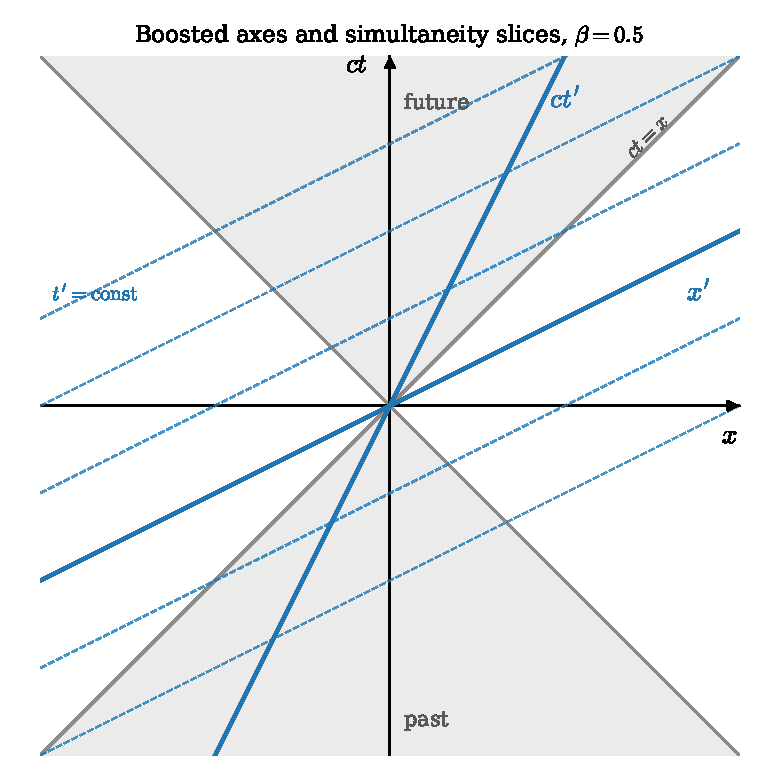
\includegraphics[width=0.60\textwidth]{fig_lightcone_simultaneity.pdf}
  \caption{The $(x, ct)$ plane with the light cone of the origin (gray)
  and the axes of a frame boosted to $\beta = 0.5$ (blue). The $ct'$ axis
  is the worldline of the moving origin, $x = \beta\,ct$; the $x'$ axis
  and its dashed translates, $ct = \beta x + \mathrm{const}$, are the
  moving observer's surfaces of simultaneity,
  Eq.~\eqref{eq:simultaneity}. Both axes close symmetrically onto the
  light cone, which is shared by all frames.}
  \label{fig:lightcone}
\end{figure}

\paragraph{Time dilation.} Take one clock at rest in $S'$, sitting at
$x' = 0$, and let it tick twice, the ticks separated by $\Delta t'$ ---
an interval of \emph{proper time}, time measured by a clock present at
both events. What does $S$ record between the same two ticks? Use the
inverse of \eqref{eq:lorentz} (i.e.\ $\beta \to -\beta$) with
$\Delta x' = 0$:
\begin{equation}
  \boxed{\;
  \Delta t = \gamma\,\Delta t' \;\ge\; \Delta t' .
  \;}
  \label{eq:time-dilation}
\end{equation}
A moving clock ticks slowly by the factor $\gamma$. The statement is
reciprocal --- each frame sees the other's clocks run slow --- and the
reciprocity is consistent precisely because the two frames disagree about
which distant events are simultaneous, Eq.~\eqref{eq:simultaneity}: the
two measurements compare one clock against \emph{different pairs} of
synchronized clocks.

\paragraph{Length contraction.} Take a rod at rest in $S'$, occupying
$x' \in [0, L_0]$; $L_0$ is its \emph{proper length}. To measure its
length in $S$ one must mark the positions of both ends \emph{at the same
$S$-time} --- length measurement of a moving object is a
simultaneity-laden operation, which is the warning that a frame-dependent
answer is coming. Set $\Delta t = 0$ in the second equation of
\eqref{eq:lorentz}: $\Delta x' = \gamma\,\Delta x$, with
$\Delta x' = L_0$ and $\Delta x = L$ the measured length. Hence
\begin{equation}
  \boxed{\;
  L = \frac{L_0}{\gamma} \;\le\; L_0 .
  \;}
  \label{eq:length-contraction}
\end{equation}
A moving rod is short by the factor $\gamma$, along its direction of
motion only (the transverse coordinates are untouched,
Appendix~\ref{app:linearity}).

\begin{example}[Cosmic-ray muons: the worked number]\label{ex:muon}
Muons are produced by cosmic-ray collisions at altitude
$h \approx 15\,\mathrm{km}$, with proper lifetime
$\tau = 2.197\,\mu\mathrm{s}$, and arrive at the ground copiously ---
which, pre-relativity, is impossible. Take $\beta = 0.995$, so
$\gamma = (1 - 0.995^2)^{-1/2} = 10.0$.

\emph{Without time dilation}, the characteristic decay length is
\begin{equation}
  \beta c\,\tau
  = 0.995 \times (2.998\times 10^8\,\mathrm{m/s})
  \times (2.197\times 10^{-6}\,\mathrm{s})
  = 655\,\mathrm{m},
\end{equation}
and the surviving fraction after $15\,\mathrm{km}$ is
$\exp(-15\,000/655) = \ee^{-22.9} \approx 1.1\times 10^{-10}$:
effectively none.

\emph{With time dilation}, the lab-frame lifetime is $\gamma\tau$
(Eq.~\eqref{eq:time-dilation}: the muon's decay clock is a moving clock),
the decay length is $\gamma\beta c\,\tau = 6.56\,\mathrm{km}$, and the
surviving fraction is
$\exp(-15\,000/6560) = \ee^{-2.29} \approx 0.10$: one in ten arrives,
consistent with observation. The two exponential laws are plotted in
Fig.~\ref{fig:muon}; at ground level they disagree by \emph{nine orders
of magnitude}.

The same arithmetic in the muon's own frame is length contraction: the
muon's clock runs normally, but the atmosphere is a moving object of
proper thickness $15\,\mathrm{km}$, contracted to
$15\,\mathrm{km}/\gamma = 1.5\,\mathrm{km}$
(Eq.~\eqref{eq:length-contraction}) --- about $2.3$ decay lengths, and
$\ee^{-2.3} \approx 0.10$ again. One phenomenon, two accounts, one
answer: the consistency is Theorem~\ref{thm:interval} at work.
\end{example}

\begin{figure}[htbp]
  \centering
  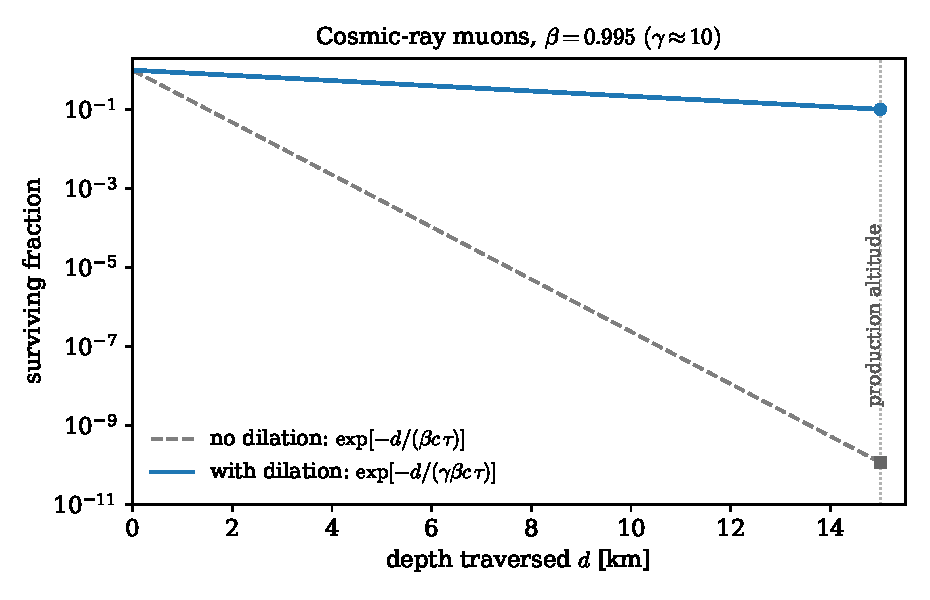
\includegraphics[width=0.75\textwidth]{fig_muon_survival.pdf}
  \caption{Surviving fraction of cosmic-ray muons ($\beta = 0.995$)
  versus traversed depth, from the exact exponential laws of
  Example~\ref{ex:muon}. Note the logarithmic scale: at
  $15\,\mathrm{km}$ the prediction without time dilation (gray, dashed)
  is wrong by nine orders of magnitude.}
  \label{fig:muon}
\end{figure}

\subsection{Where this leaves the wave equation}
\label{sec:wave-revisited}

Return to the opening problem. The wave equation
\eqref{eq:wave-eq} is not Galilean invariant --- and now we know it was
never supposed to be. The transformation that matters is
\eqref{eq:lorentz}, and under \emph{it} the operator
$\frac{1}{c^2}\partial_t^2 - \partial_x^2$ is form-invariant, as
\S\ref{sec:minkowski} will show in one line once the four-dimensional
gradient is available. Two waves, two conclusions:

\begin{itemize}
  \item \textbf{Light} obeys a wave equation with the invariant speed
  $c$. Lorentz invariance is exact, there is no medium, and the equation
  holds in the same form for every inertial observer.
  \item \textbf{Sound} obeys a wave equation with $c_s = \sqrt{T/\mu}$
  --- formally the same equation, and formally invariant under
  ``Lorentz'' transformations built with $c_s$ in place of $c$. But this
  invariance is an accident of the long-wavelength description and is
  \emph{physically broken}: the medium has a rest frame, detectable by
  any observer (measure the sound speed in two directions), and the
  microscopic chain [Osc.\ \S8] is not invariant at all --- its
  dispersion relation deviates from $\omega = c_s k$ at wavelengths
  approaching the lattice spacing.
\end{itemize}

\noindent
This distinction --- exact versus emergent, broken-by-the-medium symmetry
--- returns in \S\ref{sec:field-variational} when the string is
re-derived from a Lagrangian, and it sharpens the question Part II
answers: \emph{what does a field theory look like when Lorentz invariance
is exact and fundamental?} The simplest answer is the
Klein--Gordon field of \S\ref{sec:klein-gordon}.

%=======================================================================
\section{Minkowski Geometry and Four-Vectors}
%=======================================================================
\label{sec:minkowski}

Section~\ref{sec:postulates} did everything in the $(ct, x)$ plane with
bare hands. This section builds the apparatus that makes the same
physics effortless in four dimensions --- the metric, index gymnastics,
four-vectors, tensors --- and uses it to deliver two results promised
earlier: the invariance
of the wave operator (\S\ref{sec:wave-revisited}), and the
Doppler factor (Remark~\ref{rem:eigen}). It closes with the
structure of the Lorentz group and the switch to natural units.

\subsection{The metric and index gymnastics}
\label{sec:index-gymnastics}

An event is now a \emph{four-vector} of coordinates,
\begin{equation}
  x^\mu = (x^0, x^1, x^2, x^3) = (ct,\, x,\, y,\, z),
\end{equation}
the index written \emph{upstairs}; such components are called
\emph{contravariant}. The interval of Theorem~\ref{thm:interval},
extended to all four dimensions (the transverse directions enter with
minus signs, being ordinary Euclidean lengths --- Appendix
\ref{app:linearity} showed they are untouched by the boost), is encoded
by the \emph{Minkowski metric} of Convention~\ref{conv:signature}:
\begin{equation}
  \boxed{\;
  s^2 \;=\; \eta_{\mu\nu}\, x^\mu x^\nu
  \;=\; (x^0)^2 - (x^1)^2 - (x^2)^2 - (x^3)^2,
  \qquad
  \eta_{\mu\nu} = \operatorname{diag}(+1, -1, -1, -1).
  \;}
  \label{eq:metric-interval}
\end{equation}
Following Convention~\ref{conv:summation}, both $\mu$ and $\nu$ are
summed; the reader meeting the convention for the first time should
expand \eqref{eq:metric-interval} once by hand --- sixteen terms, twelve
of which vanish because $\eta$ is diagonal --- and never again.

The metric converts upstairs indices to downstairs ones and back.
Define the \emph{covariant} components
\begin{equation}
  x_\mu = \eta_{\mu\nu}\, x^\nu = (ct,\, -x,\, -y,\, -z),
\end{equation}
--- lowering an index costs a sign on the spatial components --- and
let $\eta^{\mu\nu}$ denote the matrix inverse of $\eta_{\mu\nu}$,
\begin{equation}
  \eta^{\mu\rho}\,\eta_{\rho\nu} = \delta^\mu_{\ \nu},
  \qquad
  \eta^{\mu\nu} = \operatorname{diag}(+1, -1, -1, -1)
\end{equation}
(numerically the same matrix in these coordinates --- a coincidence of
the diagonal form, not a general fact). \emph{Inverse} is not a
choice: demanding that raising undo lowering ---
$\eta^{\mu\nu}(\eta_{\nu\rho}x^\rho) = x^\mu$ for every $x$ --- is
verbatim the statement $\eta^{\mu\nu}\eta_{\nu\rho} =
\delta^\mu{}_\rho$, and the inverse exists, uniquely, because the
metric is \emph{nondegenerate}, $\det\eta = -1 \neq 0$ --- a genuine
requirement, since a degenerate metric would lower indices
irreversibly. Then $\eta^{\mu\nu}$ raises
indices, $x^\mu = \eta^{\mu\nu} x_\nu$, and the two operations are
inverse to each other.

\begin{remark}[What the names mean]\label{rem:contra-co}
``Contravariant'' and ``covariant'' are not decorations; they name two
opposite transformation behaviors, and the reference point of the
``co-'' and ``contra-'' is the \emph{basis}. Expand a vector on basis
vectors, $x = x^\mu e_\mu$; the vector itself is a geometric object
that does not care about frames, so if the components change by
$x'^\mu = \Lambda^\mu{}_\nu x^\nu$, the basis vectors must change by
exactly the inverse, $e'_\mu = (\Lambda^{-1})^\nu{}_\mu\, e_\nu$, for
the expansion to keep describing the same object. Quantities
transforming like the basis --- with $\Lambda^{-1}$ --- \emph{co}-vary
with it and are called covariant; quantities transforming with
$\Lambda$ vary \emph{contra} to it. (\S\ref{sec:gradient} shows the
gradient is the natural citizen of the covariant class, and
\S\ref{sec:tensors} takes the two behaviors as the prototypes for the
whole tensor hierarchy.) In special relativity the distinction is
bookkeeping rather than content --- the metric converts either version
into the other at the cost of spatial signs, so $x^\mu$ and $x_\mu$
carry the same information --- but the bookkeeping is load-bearing:
Convention~\ref{conv:summation} sums only upper-lower pairs, and
\S\ref{sec:tensors} shows that pairing is precisely the one whose
transformation factors cancel.
\end{remark}

\noindent
The general \emph{inner product} of four-vectors
and its expansion in $3+1$ language:
\begin{equation}
  \boxed{\;
  a \cdot b \;\equiv\; \eta_{\mu\nu}\, a^\mu b^\nu
  \;=\; a^\mu b_\mu \;=\; a_\mu b^\mu
  \;=\; a^0 b^0 - \vec a \cdot \vec b .
  \;}
  \label{eq:inner-product}
\end{equation}

Which linear maps preserve this structure? Write
\begin{equation}
  x'^\mu = \Lambda^\mu{}_\nu\, x^\nu .
\end{equation}
Demanding $s'^2 = s^2$ for \emph{every} event $x$ forces, by the
polarization identity
$a \cdot b = \tfrac14\bigl[(a+b)^2 - (a-b)^2\bigr]$, the invariance of
every inner product, and hence the condition on the matrix alone:
\begin{equation}
  \boxed{\;
  \eta_{\mu\nu}\, \Lambda^\mu{}_\rho\, \Lambda^\nu{}_\sigma
  = \eta_{\rho\sigma}
  \qquad\text{(defining condition of a Lorentz transformation).}
  \;}
  \label{eq:lorentz-condition}
\end{equation}
Three immediate consequences of \eqref{eq:lorentz-condition} are
collected here, before anything is built on top, because the entire
calculus of Part I leans on them.

\emph{(i) Matrix form.} With $\mathsf\Lambda$ the matrix
$[\Lambda^\mu{}_\nu]$ (row $\mu$, column $\nu$) and $\boldsymbol\eta$
the matrix of the metric,
\begin{equation}
  \boxed{\;
  \mathsf\Lambda^{\mathsf T}\,
  \boldsymbol\eta\,
  \mathsf\Lambda
  = \boldsymbol\eta
  \;}
  \label{eq:lorentz-matrix}
\end{equation}
--- the spacetime analogue of $R^{\mathsf T}R = \mathsf 1$ for
rotations, with $\eta$ replacing the identity as the preserved
bilinear form. Note carefully: the \emph{transpose}, not the inverse,
sits on the left. The superficially similar
$\mathsf\Lambda^{-1}\boldsymbol\eta\,\mathsf\Lambda = \boldsymbol\eta$
would assert that $\boldsymbol\eta$ \emph{commutes} with every
Lorentz transformation, which is already false for a single boost
(check the $2\times2$ blocks: $\boldsymbol\eta\mathsf\Lambda$ flips
the sign of $\mathsf\Lambda$'s spatial rows,
$\mathsf\Lambda\boldsymbol\eta$ of its spatial columns, and a boost
matrix is not invariant under that exchange).

\begin{remark}[Rotations and Lorentz transformations: one template]
\label{rem:one-template}
Equation \eqref{eq:lorentz-matrix} is one instance of a template
worth seeing whole. For any fixed invertible symmetric matrix
$\mathsf G$, the solutions of
\begin{equation}
  \mathsf M^{\mathsf T}\,\mathsf G\,\mathsf M = \mathsf G
\end{equation}
are exactly the linear maps preserving the bilinear form
$\langle x, y\rangle = x^{\mathsf T}\mathsf G\, y$, and they always
form a group. The choice $\mathsf G = \mathsf 1$ in $n$ dimensions
gives $R^{\mathsf T}R = \mathsf 1$ --- the orthogonal group $O(n)$,
rotations and reflections, preservers of Euclidean length. The choice
$\mathsf G = \boldsymbol\eta$ gives the Lorentz group, in this
classification named $O(1,3)$ --- one plus sign, three minus signs
--- and the general signature $\mathsf G =
\operatorname{diag}(+\cdots+,-\cdots-)$ gives the family $O(p,q)$.
Two things are \emph{shared} across the family, and everything else
divides along the signs of $\mathsf G$.

Shared: the constraint counting --- the template is a symmetric
matrix equation, $n(n{+}1)/2$ conditions on $n^2$ entries, leaving
$n(n{-}1)/2$ parameters, one per coordinate plane. For $n = 4$ that
is $6$ for the rotation group $O(4)$ and $6$ for the Lorentz group
alike: \emph{same number of planes, same dimension} (the count is
signature-blind; \S\ref{sec:lorentz-group} spends the Lorentz six as
three rotations plus three boosts). Shared too: $\det\mathsf M =
\pm1$, by taking determinants of the template.

Divided by the sign, with each division already witnessed in this
document:
\begin{itemize}
  \item \textbf{Bounded versus unbounded.} A rotation angle lives on
  a circle; the rapidity lives on $\R$
  (Remark~\ref{rem:sanity}(iii)), $\cosh\phi$ is unbounded where
  $\cos\theta$ is trapped in $[-1,1]$, and correspondingly $O(4)$ is
  a \emph{compact} group (closed and bounded as a set of matrices)
  while $O(1,3)$ is not --- there is no largest boost, and the group
  is unbounded as a set of matrices. Most of what makes Lorentz
  representation theory harder than rotation representation theory
  descends from this single property. [stated; QFT-course territory.]
  \item \textbf{Eigenvalues.} Rotations have unit-modulus eigenvalues
  $\ee^{\pm\ii\theta}$; boosts have real reciprocal ones
  $\ee^{\pm\phi}$, with null eigenvectors ---
  Remark~\ref{rem:eigen}, now recognizable as the $\mathsf G$-sign
  showing up in a characteristic polynomial.
  \item \textbf{How many pieces.} $O(n)$ has two connected components
  ($\det = \pm1$); $O(1,3)$ has \emph{four}
  (\S\ref{sec:lorentz-group}), and the doubling has a clean geometric
  cause: the Euclidean ``unit sphere'' $\{x : \langle x,x\rangle = 1\}$
  is connected, but its Minkowski counterpart is the two-sheeted
  hyperboloid $t^2 - |\vx|^2 = 1$ of Fig.~\ref{fig:hyperbolae} ---
  and since a continuous family of transformations can never carry a
  unit timelike vector from one sheet to the other, ``which sheet''
  is a second discrete invariant, alongside $\det$. That is the
  invariant \S\ref{sec:lorentz-group} will meet as
  $\operatorname{sgn}\Lambda^0{}_0$.
\end{itemize}
One more choice of $\mathsf G$ completes the family: take $\mathsf G$
\emph{antisymmetric} and the template names the symplectic group ---
whose preserved pairing is exactly the $(q, p)$ structure underlying
the Poisson bracket, so that the canonical transformations of
[Mech.\ \S8] are this same template's third appearance in the series.
[stated; not developed further here.]
\end{remark}

\emph{(ii) The inverse, without inverting.} Apply the raising and
lowering machinery to $\Lambda$ itself: define
$\Lambda_\mu{}^\nu \equiv
\eta_{\mu\rho}\,\Lambda^\rho{}_\sigma\,\eta^{\sigma\nu}$, and
contract the defining condition \eqref{eq:lorentz-condition} with
$\eta^{\sigma\nu}$:
\begin{equation}
  \eta_{\alpha\beta}\,\Lambda^\alpha{}_\rho\,
  \Lambda^\beta{}_\sigma\,\eta^{\sigma\nu}
  = \eta_{\rho\sigma}\,\eta^{\sigma\nu}
  = \delta_\rho{}^\nu
  \qquad\Longrightarrow\qquad
  \Lambda_\alpha{}^\nu\;\Lambda^\alpha{}_\rho
  = \delta^\nu{}_\rho ,
\end{equation}
i.e.
\begin{equation}
  \boxed{\;
  \bigl(\Lambda^{-1}\bigr)^\nu{}_\mu
  \;=\;
  \Lambda_\mu{}^\nu :
  \;}
  \label{eq:inverse-is-lowered}
\end{equation}
\emph{the inverse transformation is the index-lowered transpose}, and
no matrix inversion is ever needed. This document adopts
\eqref{eq:inverse-is-lowered} as standing notation: from here on the
inverse is always written $\Lambda_\mu{}^\nu$, the index positions
doing the inverting silently. The horizontal order of $\Lambda$'s
slots is therefore load-bearing --- $\Lambda^\mu{}_\nu$ and
$\Lambda_\nu{}^\mu$ are inverse-transposes of one another, not the
same array, and stacking the indices vertically would destroy the
distinction.

\emph{(iii) Lowering commutes with transforming.} The covariant
components $x_\mu = \eta_{\mu\nu}x^\nu$ were defined by the metric;
do they inherit a coherent transformation law? Transform the lowered
object, and rewrite using \eqref{eq:inverse-is-lowered}:
\begin{equation}
  a'_\mu
  = \eta_{\mu\nu}\, a'^\nu
  = \eta_{\mu\nu}\,\Lambda^\nu{}_\rho\,\eta^{\rho\sigma} a_\sigma
  = \Lambda_\mu{}^\sigma\, a_\sigma :
  \label{eq:lowered-transform}
\end{equation}
lowered components transform with the \emph{inverse} --- with the
basis, in the language of Remark~\ref{rem:contra-co}, whose
``covariant'' label is hereby proved rather than assigned. Lowering
first and transforming second agrees with transforming first and
lowering second, and the agreement is
\eqref{eq:lorentz-condition} once more: one condition, read three
ways --- inner products preserved, the metric unmoved, index
gymnastics frame-proof.

Section~\ref{sec:lorentz-group} mines \eqref{eq:lorentz-matrix} for
the structure of the group. Meanwhile, a \emph{four-vector} is, by
definition, any quadruple $a^\mu$ that
transforms like the coordinates, $a'^\mu = \Lambda^\mu{}_\nu a^\nu$
(the definition is systematized, and extended to tensors of arbitrary
rank, in \S\ref{sec:tensors});
Eq.~\eqref{eq:lorentz-condition} then guarantees that $a \cdot b$ is the
same number in every frame --- a \emph{Lorentz invariant} (or
\emph{scalar}). The strategy for the rest of Part I is now set:
\emph{build the objects of mechanics out of four-vectors, and equations
between four-vectors will hold in every frame at once.}

\subsection{Causal structure and proper time}
\label{sec:causal-structure}

The sign of the interval sorts pairs of events into three invariant
classes --- invariant because $\Delta s^2$ is, Theorem~\ref{thm:interval}:
\begin{center}
\begin{tabular}{lll}
\toprule
class & condition & invariant meaning \\
\midrule
timelike & $\Delta s^2 > 0$ & a slower-than-light traveler can attend both events \\
lightlike (null) & $\Delta s^2 = 0$ & exactly a light signal connects them \\
spacelike & $\Delta s^2 < 0$ & no signal connects them; causally independent \\
\bottomrule
\end{tabular}
\end{center}
Two useful normal forms, each a one-line boost exercise: for a timelike
pair there is a frame in which both events happen \emph{at the same
place}, separated by pure time
$\Delta t = \sqrt{\Delta s^2}/c$; for a spacelike pair, a frame in which
they are \emph{simultaneous}, separated by pure distance
$\sqrt{-\Delta s^2}$. (For the timelike case, boost with
$\beta = \Delta x/(c\Delta t)$, which is $< 1$ precisely because the
pair is timelike; the spacelike case uses
$\beta = c\Delta t/\Delta x$.) In the spacelike case the \emph{time
order} of the two events is frame-dependent --- there are frames in
which either precedes the other --- which is why any signal between
spacelike-separated events would be a causality violation for some
observer, and why the light cone of Fig.~\ref{fig:lightcone} is the
absolute causal boundary: the future and past cones are
frame-independent regions, and ``elsewhere'' is negotiable only in
time-ordering, never in reachability.

Now promote the interval from pairs of events to \emph{worldlines}. A
material particle traces a curve $x^\mu(t)$ whose every segment is
timelike ($|\vec v| < c$); the interval along an infinitesimal segment,
\begin{equation}
  c^2\,\dd\tau^2 \;\equiv\; \dd s^2
  = c^2\dd t^2 - |\dd\vx|^2
  = c^2\dd t^2\left(1 - \beta(t)^2\right),
\end{equation}
defines the \emph{proper time} $\dd\tau$: the time elapsed on an ideal
clock riding the segment, since in the clock's momentary rest frame
$\dd\vx = 0$ and $\dd s^2 = c^2 \dd t_{\text{rest}}^2$. Integrating,
\begin{equation}
  \boxed{\;
  \tau \;=\; \int \dd\tau
  \;=\; \int \frac{\dd t}{\gamma(t)},
  \qquad
  \gamma(t) = \frac{1}{\sqrt{1 - \beta(t)^2}} .
  \;}
  \label{eq:proper-time}
\end{equation}
Proper time is a Lorentz scalar --- all observers agree on what a given
clock reads --- and it is the natural parameter along any timelike
worldline, a role it takes up in \S\ref{sec:four-velocity} and keeps for
the rest of the document.

\begin{remark}[The clock hypothesis]\label{rem:clock-hypothesis}
Equation \eqref{eq:proper-time} asserts that a clock's rate depends on
its instantaneous \emph{speed} and not separately on its acceleration.
This is an additional physical assumption --- special relativity as
derived in \S\ref{sec:postulates} relates inertial frames only --- and
an experimentally supported one: muons circulating in storage rings at
$\gamma \approx 29$, under centripetal accelerations of order
$10^{18}\,g$, show lifetimes dilated by exactly $\gamma$ with no
acceleration correction. [experimental input.]
\end{remark}

\begin{remark}[The twin ``paradox'']\label{rem:twin}
Between two fixed timelike-separated events $A$ and $B$, different
worldlines accumulate \emph{different} proper times, and the straight
(inertial) worldline accumulates the \emph{most}. Proof: work in the
frame where the straight worldline is at rest, so its proper time is
the full coordinate time, $\tau_{\text{straight}} = \Delta t$; any
other worldline between the same events has
$\dd\tau = \dd t/\gamma \le \dd t$ everywhere, with strict inequality
wherever it moves. Hence the traveling twin --- outbound, turn, return
--- ages less than the stay-at-home twin
(Fig.~\ref{fig:twin}): with $\beta = 0.6$ on both legs,
$\tau_{\text{travel}} = \tau_{\text{home}}/\gamma = 0.8\,
\tau_{\text{home}}$. This is the \emph{reversed triangle inequality} of
Minkowski geometry --- the straight path is longest, the single sign in
the metric again --- and there is no paradox to resolve: the two
worldlines are not symmetric, one is straight and one is kinked, and
straightness (inertia) is frame-independent. The traveler's turnaround
is the geometric fact every observer agrees on.
\end{remark}

\begin{figure}[htbp]
  \centering
  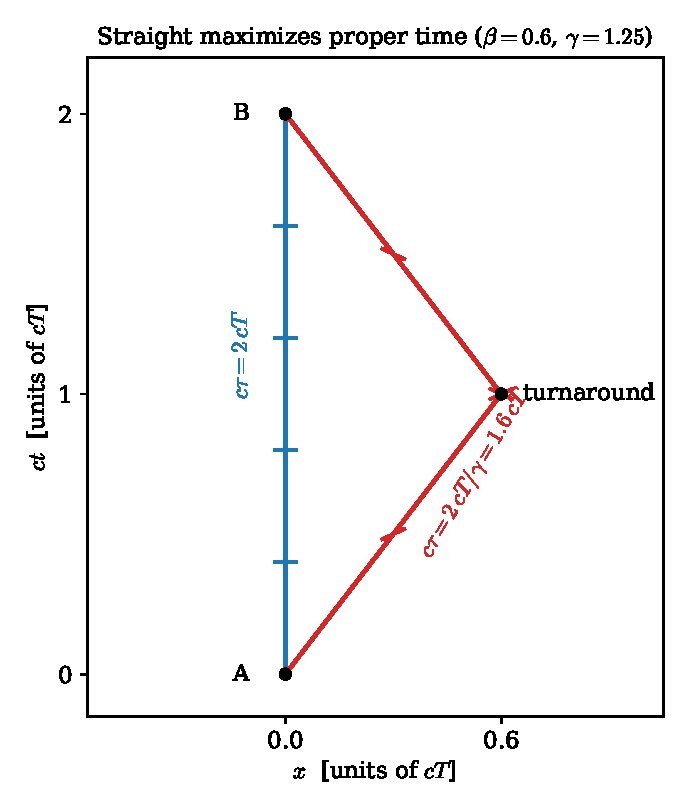
\includegraphics[width=0.5\textwidth]{fig_twin_proper_time.pdf}
  \caption{Two worldlines between the same events $A$ and $B$. Tick
  marks are placed at equal intervals of \emph{proper} time,
  $c\,\Delta\tau = 0.4\,cT$, computed from
  Eq.~\eqref{eq:proper-time}: five intervals fit on the straight
  worldline, four on the kinked one ($\beta = 0.6$,
  $\gamma = 1.25$).}
  \label{fig:twin}
\end{figure}

\begin{example}[GPS clocks: the worked number]\label{ex:gps}
A GPS satellite orbits at $r = 26\,571\,\mathrm{km}$ with speed
$v = \sqrt{GM_\oplus/r} = 3.87\,\mathrm{km/s}$, i.e.\
$\beta = 1.29\times 10^{-5}$. By Eq.~\eqref{eq:proper-time} its clock
runs slow relative to ground clocks by the fraction
\begin{equation}
  1 - \frac{1}{\gamma} \approx \frac{\beta^2}{2}
  = 8.3\times 10^{-11},
\end{equation}
which over one day ($86\,400\,\mathrm{s}$) accumulates to
$7.2\,\mu\mathrm{s}$ --- and a timing error of $7.2\,\mu\mathrm{s}$ is
a ranging error of $c \times 7.2\,\mu\mathrm{s} \approx 2\,\mathrm{km}$.
GPS would be useless within hours if this were not corrected.
(Gravitational time dilation --- general relativity --- pushes the
other way and harder, $+45.9\,\mu\mathrm{s}$ per day, for a net
satellite clock \emph{gain} of $38.7\,\mu\mathrm{s}$ per day; the
system corrects for both. [stated; the gravitational part is outside
this document's scope.])
\end{example}

\subsection{Four-velocity and four-acceleration}
\label{sec:four-velocity}

The ordinary velocity $\dd x^\mu/\dd t$ is \emph{not} a four-vector:
$t$ is the zeroth \emph{component} of $x^\mu$, not a scalar, so dividing
by $\dd t$ ruins the transformation law. The fix is to differentiate
with respect to the scalar the worldline carries with it --- proper
time:
\begin{equation}
  \boxed{\;
  u^\mu \;\equiv\; \tot{x^\mu}{\tau}
  = \gamma\,\tot{x^\mu}{t}
  = \gamma\,(c,\, \vec v),
  \;}
  \label{eq:four-velocity}
\end{equation}
using $\dd t = \gamma\,\dd\tau$ from \eqref{eq:proper-time}. Its norm
is fixed once and for all:
\begin{equation}
  u \cdot u
  = \gamma^2\bigl(c^2 - |\vec v|^2\bigr)
  = \gamma^2 c^2 \bigl(1 - \beta^2\bigr)
  = c^2 .
  \label{eq:u-norm}
\end{equation}
Every four-velocity is a unit timelike vector (in units of $c$): the
``speed through spacetime'' is not a degree of freedom, and the
constraint has a derivative worth keeping. Defining the
four-acceleration $a^\mu = \dd u^\mu/\dd\tau$ and differentiating
\eqref{eq:u-norm} along the worldline:
\begin{equation}
  0 = \tot{}{\tau}(u \cdot u) = 2\, a \cdot u
  \qquad\Longrightarrow\qquad
  \boxed{\; a \cdot u = 0 : \;}
  \label{eq:a-perp-u}
\end{equation}
four-acceleration is always Minkowski-orthogonal to four-velocity ---
acceleration can rotate the four-velocity on its hyperboloid
$u \cdot u = c^2$ but never change its length. Both facts return in
\S\ref{sec:relativistic-particle}, where $mu^\mu$ becomes the
four-momentum and \eqref{eq:u-norm} becomes the mass shell.

\subsection{The Doppler effect from the null eigenvalue}
\label{sec:doppler}

Remark~\ref{rem:eigen} stated without proof that the boost eigenvalue
$\ee^{\phi}$ is the relativistic Doppler factor. The derivation is two
lines precisely \emph{because} it runs along the eigendirection.

A source at rest at the origin of $S$ emits light pulses toward $+x$ at
proper period $T$: emission events $(ct, x) = (cnT, 0)$,
$n = 0, 1, 2, \dots$ Each pulse travels the ray
$x = x_0 + c(t - t_0)$, along which the null coordinate
$u = ct - x$ is \emph{constant}; the $n$-th pulse is the line
$u = cnT$, so successive pulses are separated by
\begin{equation}
  \Delta u = cT .
\end{equation}
An observer receding at velocity $\beta$ is at rest in the boosted
frame $S'$; by Eq.~\eqref{eq:null-boost}, the pulse spacing in her null
coordinate is the eigenvalue-stretched
\begin{equation}
  \Delta u' = \ee^{\phi}\, \Delta u = \ee^{\phi}\, cT .
\end{equation}
She receives the pulses at a fixed position, $\Delta x' = 0$, so the
period she measures is
$c\,\Delta t'_{\text{rec}} = \Delta(ct' - x') = \Delta u'$. Hence
\begin{equation}
  \boxed{\;
  \frac{T_{\text{obs}}}{T_{\text{src}}}
  = \ee^{\phi}
  = \sqrt{\frac{1+\beta}{1-\beta}},
  \qquad
  \frac{f_{\text{obs}}}{f_{\text{src}}}
  = \ee^{-\phi}
  = \sqrt{\frac{1-\beta}{1+\beta}}
  \;}
  \label{eq:doppler}
\end{equation}
--- redshift for recession ($\phi > 0$), blueshift for approach
($\beta \to -\beta$ flips the exponent), and successive recessions
compound by \emph{multiplying} the factors, i.e.\ adding rapidities:
Doppler shifts of collinear relative motions compose exactly as
Remark~\ref{rem:eigen} promised eigenvalues would.

\begin{remark}[Against the nonrelativistic Doppler formulas]
The classical Doppler effect for sound has \emph{two} formulas ---
moving source, $f_{\text{obs}} = f_{\text{src}}/(1 + \beta_s)$, versus
moving observer, $f_{\text{obs}} = f_{\text{src}}(1 - \beta_o)$ ---
distinguishable because the medium's rest frame settles who is
``really'' moving. Equation \eqref{eq:doppler} is a single formula
depending only on the \emph{relative} velocity, and expanding it,
$\ee^{-\phi} = 1 - \beta + \tfrac12\beta^2 - \dots$, it interpolates
between the two classical answers, splitting the difference at second
order. With no medium, no such distinction survives: this is
Postulate~\ref{post:relativity} showing up in a lineshape. There is
also a purely relativistic \emph{transverse} Doppler shift, a factor
$1/\gamma$ at closest approach with no classical analogue at all ---
it is time dilation \eqref{eq:time-dilation} observed directly.
\end{remark}

\subsection{The spacetime gradient and the d'Alembertian}
\label{sec:gradient}

One more object completes the kit: differentiation. Define
\begin{equation}
  \partial_\mu \;\equiv\; \pd{}{x^\mu}
  = \left(\frac{1}{c}\pd{}{t},\; \nabla\right).
\end{equation}
Why the \emph{downstairs} index? Chain rule: under
$x'^\mu = \Lambda^\mu{}_\nu x^\nu$,
\begin{equation}
  \partial'_\mu
  = \pd{}{x'^\mu}
  = \pd{x^\nu}{x'^\mu}\,\pd{}{x^\nu}
  = \Lambda_\mu{}^\nu\, \partial_\nu :
  \label{eq:gradient-transform}
\end{equation}
the gradient transforms with the \emph{inverse} matrix, in the
notation of \eqref{eq:inverse-is-lowered} --- precisely the behavior
\eqref{eq:lowered-transform} established for lowered components, so
the index placement is derived, not decorative. (Check the logic of
\eqref{eq:gradient-transform}: the old coordinates as functions of
the new are
$x^\nu = \Lambda_\mu{}^\nu\, x'^\mu$, whence the Jacobian.)
Raising the index, $\partial^\mu = \eta^{\mu\nu}\partial_\nu = 
(\tfrac1c \partial_t, -\nabla)$, and contracting gradient with
gradient produces a scalar operator, the \emph{d'Alembertian}:
\begin{equation}
  \boxed{\;
  \Box \;\equiv\; \partial_\mu \partial^\mu
  = \frac{1}{c^2}\pd{^2}{t^2} - \nabla^2 .
  \;}
  \label{eq:dalembertian}
\end{equation}
Because it is a full contraction of Lorentz-covariant objects, $\Box$
is the same operator in every inertial frame --- the promise of
\S\ref{sec:wave-revisited} is now a one-line theorem. The wave equation
for light, $\Box\,\varphi = 0$, is manifestly form-invariant under
Lorentz transformations, in exactly the way
Eq.~\eqref{eq:wave-not-invariant} showed it fails to be under Galilean
ones; and when field theory needs a relativistic equation of motion in
\S\ref{sec:klein-gordon}, $\Box$ will be the only two-derivative
scalar operator available.

\subsection{Scalars, vectors, tensors, and the covariance principle}
\label{sec:tensors}

The words ``scalar'' and ``four-vector'' have so far been used
case-by-case. Before dynamics begins, it is worth assembling the full
hierarchy once, systematically --- because the central objects ahead
carry \emph{two} indices (the field tensor $F_{\mu\nu}$ unifying
$\vE$ and $\vB$, the energy-momentum tensor $T^{\mu\nu}$), and the
reasoning that will certify them deserves to be set up properly rather
than improvised on arrival.

\paragraph{The two prototype behaviors.} Everything descends from two
objects already in hand. The coordinate displacement transforms with
$\Lambda$,
\begin{equation}
  \dd x'^\mu = \Lambda^\mu{}_\nu\, \dd x^\nu
  \qquad\text{(contravariant prototype)},
\end{equation}
and the gradient transforms with the inverse,
Eq.~\eqref{eq:gradient-transform},
\begin{equation}
  \partial'_\mu = \Lambda_\mu{}^\nu\, \partial_\nu
  \qquad\text{(covariant prototype)}.
\end{equation}
Every transformation behavior in the theory is built from copies of
these two --- one copy per index, upstairs indices behaving like
$\dd x^\mu$, downstairs like $\partial_\mu$.

\begin{definition}[Lorentz scalars, vectors, tensors]
\label{def:tensor}
Under $x'^\mu = \Lambda^\mu{}_\nu x^\nu$:
\begin{itemize}
  \item a \textbf{scalar} (rank 0) is a single number assigned the same
  value in every frame: $s' = s$. Already met: the interval $s^2$,
  proper time $\tau$, the norm $u \cdot u$.
  \item a \textbf{contravariant vector} (type $(1,0)$) is a quadruple
  transforming like the displacement:
  $a'^\mu = \Lambda^\mu{}_\nu\, a^\nu$. Already met: $x^\mu$, $u^\mu$.
  \item a \textbf{covariant vector} (type $(0,1)$) transforms like the
  gradient:
  $b'_\mu = \Lambda_\mu{}^\nu\, b_\nu$ (the inverse, per
  \eqref{eq:inverse-is-lowered}). Already met:
  $\partial_\mu$, and $x_\mu = \eta_{\mu\nu}x^\nu$.
  \item a \textbf{tensor of type $(p,q)$} carries $p$ upstairs and $q$
  downstairs indices, each transforming with its prototype's factor:
  \begin{equation}
    T'^{\mu_1\cdots\mu_p}{}_{\nu_1\cdots\nu_q}
    = \Lambda^{\mu_1}{}_{\rho_1}\!\cdots\Lambda^{\mu_p}{}_{\rho_p}\,
      \Lambda_{\nu_1}{}^{\sigma_1}\!\cdots
      \Lambda_{\nu_q}{}^{\sigma_q}\;
      T^{\rho_1\cdots\rho_p}{}_{\sigma_1\cdots\sigma_q}.
    \label{eq:tensor-law}
  \end{equation}
  Scalars and vectors are the ranks $(0,0)$, $(1,0)$, $(0,1)$ of the
  one definition.
\end{itemize}
\end{definition}

\paragraph{Why this law and no other.} Equation \eqref{eq:tensor-law}
is not an arbitrary decoration; it is the \emph{unique} linear
transformation behavior under which index contraction produces
frame-independent physics. The engine is one cancellation:

\begin{proposition}[Contraction]\label{prop:contraction}
Setting one upstairs index of a tensor equal to one downstairs index
and summing yields a tensor of type $(p{-}1, q{-}1)$. In particular, a
full contraction --- no free indices --- is a scalar.
\end{proposition}

\begin{proof}
It suffices to watch one contracted pair; spectator indices carry
their factors along unchanged. For a $(1,1)$ tensor, contract and
transform:
\begin{equation}
  T'^{\mu}{}_{\mu}
  = \Lambda^\mu{}_\rho\,\Lambda_\mu{}^\sigma\;
    T^{\rho}{}_{\sigma}
  = \delta_\rho{}^{\sigma}\, T^{\rho}{}_{\sigma}
  = T^{\rho}{}_{\rho} :
\end{equation}
the $\Lambda$ of the upstairs slot annihilates the
$\Lambda_\mu{}^\sigma$ of the downstairs slot, by
\eqref{eq:inverse-is-lowered}. This is why every invariant met so far ---
$a \cdot b = a^\mu b_\mu$, $s^2$, $u \cdot u$, $\Box$ acting on a
scalar --- was an upper-lower contraction: the pairing of the two
prototype behaviors is precisely the pairing that cancels.
\end{proof}

\noindent
Read backwards, this \emph{derives} the definition: demand that
upstairs and downstairs indices exist, that contracting them yields
invariants, and that the behavior be linear --- then each upstairs
index must carry $\Lambda$ exactly where each downstairs index carries
the inverse $\Lambda_\nu{}^\sigma$, which is
Eq.~\eqref{eq:tensor-law}.

\paragraph{Where higher ranks come from.} Two mechanisms manufacture
tensors of rank $\ge 2$, and both will be used.
\emph{Outer products}: if $a^\mu$ and $b^\nu$ are vectors, the
sixteen products $a^\mu b^\nu$ transform as a $(2,0)$ tensor ---
immediate from the definition. \emph{Linear physical laws}: whenever
physics linearly relates one vector to another, the array of
coefficients is forced to be a tensor. That is the content of:

\begin{proposition}[Quotient rule]\label{prop:quotient}
Let $T_{\mu\nu}$ be an array defined in every frame, and suppose that
for \emph{every} four-vector $a^\nu$ the contraction
$c_\mu \equiv T_{\mu\nu}a^\nu$ transforms as a covariant vector. Then
$T_{\mu\nu}$ is a $(0,2)$ tensor. (Analogous statements hold for every
index structure.)
\end{proposition}

\begin{proof}
Write what is assumed, in the primed frame and with the primed
ingredients: $T'_{\mu\nu}a'^\nu = c'_\mu$. Express the right side by
the known laws for $c$ and then $a$:
\begin{equation}
  T'_{\mu\nu}\,\Lambda^\nu{}_\sigma\, a^\sigma
  = \Lambda_\mu{}^\rho\, c_\rho
  = \Lambda_\mu{}^\rho\, T_{\rho\sigma}\, a^\sigma .
\end{equation}
This holds for \emph{arbitrary} $a^\sigma$, so the coefficients of
$a^\sigma$ agree:
$T'_{\mu\nu}\Lambda^\nu{}_\sigma
= \Lambda_\mu{}^\rho\, T_{\rho\sigma}$. Multiply by
$\Lambda_\kappa{}^\sigma$ to free the last index (using
\eqref{eq:inverse-is-lowered} in the form
$\Lambda^\nu{}_\sigma\Lambda_\kappa{}^\sigma = \delta^\nu{}_\kappa$):
$T'_{\mu\kappa} = \Lambda_\mu{}^\rho\,
\Lambda_\kappa{}^\sigma\, T_{\rho\sigma}$ --- the $(0,2)$
transformation law.
\end{proof}

\noindent
The quotient rule is how tensors are \emph{detected} in practice: one
never checks sixteen transformation equations directly. Part III runs
it verbatim --- the Lorentz force on a charge is linear in the
charge's four-velocity, so the coefficient array $F_{\mu\nu}$ is a
tensor by Proposition~\ref{prop:quotient}, and the transformation
rules of $\vE$ and $\vB$ fall out of Eq.~\eqref{eq:tensor-law} for
free. [Forward pointer: \S\ref{sec:field-tensor}.]

Sums of same-type tensors and products with scalars stay in type;
with outer products and contraction, this closes the algebra of
operations, and raising or lowering an index --- contraction with
$\eta^{\mu\nu}$ or $\eta_{\mu\nu}$ --- is a special case rather than a
new rule.

\paragraph{The invariant tensors.} Two tensors have the same
components in every frame. The metric:
$\eta'_{\rho\sigma} =
\Lambda_\rho{}^\mu\, \Lambda_\sigma{}^\nu\, \eta_{\mu\nu}
= \eta_{\rho\sigma}$, which is the defining condition
\eqref{eq:lorentz-condition} rearranged --- \emph{a Lorentz
transformation is precisely one that leaves the components of the
metric unchanged}. And the Kronecker delta $\delta^\mu{}_\nu$, whose
invariance is the statement $\Lambda\Lambda^{-1} = \mathsf 1$. These
are the index-shuffling machines available in every frame for free; a
third, the totally antisymmetric $\epsilon^{\mu\nu\rho\sigma}$
(invariant under the proper orthochronous component only), joins them
in Part III when first needed. [stated; introduced properly in
\S\ref{sec:field-tensor}.]

\paragraph{Index gymnastics is frame-proof.} One structural fact,
already proved in pieces, deserves its general statement. Because
$\eta_{\mu\nu}$ and $\eta^{\mu\nu}$ are invariant tensors,
\emph{raising or lowering any index of any tensor commutes with the
Lorentz transformation law}: gymnastics before the boost and
gymnastics after the boost give the same components --- for vectors
this was Eq.~\eqref{eq:lowered-transform}, and the general case is
the same computation with spectator indices riding along. The index
notation's entire frame-independence rests on this commutativity, and
the commutativity rests on \eqref{eq:lorentz-condition}: one
condition behind the whole calculus.

\paragraph{Fields: a tensor at every event.} Part II needs one more
notion, planted here. A \emph{scalar field} assigns a scalar to each
event: one function $\phi$ with
\begin{equation}
  \phi'(x') = \phi(x)
  \qquad\text{whenever } x' = \Lambda x
  \label{eq:scalar-field}
\end{equation}
--- the moved observer, evaluating her function at her label for the
\emph{same event}, reads the same number. A vector or tensor field
attaches the corresponding object to each event, components
transforming by Eq.~\eqref{eq:tensor-law} on top of the relabeling
\eqref{eq:scalar-field}. One consequence is used repeatedly later:
if $\phi$ is a scalar field, then $\partial_\mu\phi$ is a covariant
vector field and $\Box\phi$ is again a scalar field ---
differentiation respects the hierarchy, which is what makes it
possible to write field equations covariantly at all.

\begin{remark}[The covariance principle, and a terminological hazard]
\label{rem:covariance-principle}
The payoff of the whole subsection is one sentence. \emph{If an
equation sets equal two tensors of the same type, and it holds in one
inertial frame, it holds in every inertial frame} --- for the
difference of its two sides is a tensor whose components vanish in one
frame, and Eq.~\eqref{eq:tensor-law}, being linear, sends zero to
zero. This is the operational content of
Postulate~\ref{post:relativity} and the standing strategy of the rest
of the document: laws of physics will be written as equations between
same-type tensors (``in covariant form''), whereupon their frame
independence is automatic rather than checked. Terminology, regrettably,
overloads one word: a \emph{covariant index} is a downstairs index,
while a \emph{covariant equation} is one written in tensor form and
hence form-invariant. Both usages are standard; context separates
them.
\end{remark}

\subsection{The grammar of indices}
\label{sec:index-grammar}

The hierarchy of Definition~\ref{def:tensor} is complete, and
everything ahead computes inside it constantly. The computations obey
a small, closed set of rules --- scattered so far across conventions
and propositions; collected here once, as grammar, with the standing
traps named. Everything in this subsection is bookkeeping for
structures already established; nothing is new physics.

\paragraph{Rule 1: free and dummy indices.} In any single term, an
index appears either \emph{once} (a \emph{free} index, labeling which
component equation is meant) or \emph{exactly twice, once up and once
down} (a \emph{dummy} index, summed by Convention
\ref{conv:summation}). Grammar of equations: every term of an
equation must carry the same free indices, same letters, \emph{same
heights}. Dummies are private to their term and may be renamed at
will --- to any letter not already in use there.
\begin{gather}
  \underbrace{a^\mu = b^\mu + \Lambda^\mu{}_\nu c^\nu}_{\text{legal}}
  \qquad\quad
  \underbrace{a^\mu = b_\mu}_{\text{illegal: heights}}
  \notag\\[2pt]
  \underbrace{a^\mu = b^\nu}_{\text{illegal: free mismatch}}
  \qquad\quad
  \underbrace{a^\mu b_\mu c_\mu}_{\text{illegal: } \mu \text{ thrice}}
\end{gather}
An index appearing three times, or twice at the same height, is not
``summed anyway'' --- it is a syntax error, and in practice almost
always the fossil of a forgotten rename.

\paragraph{Rule 2: raising and lowering.} $\eta_{\mu\nu}$ lowers,
$\eta^{\mu\nu}$ raises, one slot at a time, spectator indices
untouched; in this signature the operation costs a sign on each
spatial component and nothing on the time component. Lower-then-raise
is the identity (\S\ref{sec:index-gymnastics}: the inverse property
is exactly this demand). Contraction with the metric \emph{is}
raising/lowering --- one mechanism, not two rules.
\emph{Example:} for the four-momentum $p^\mu = (E, \vp)$, lowering
gives $p_\mu = (E, -\vp)$, and the contraction is immediately useful:
$p^\mu p_\mu = E^2 - |\vp|^2$, the mass shell
\eqref{eq:mass-shell} in one line.

\paragraph{Rule 3: slot order matters.} The horizontal position of
a slot is part of a tensor's identity: $T^\mu{}_\nu$ means
$\eta^{\mu\rho}T_{\rho\nu}$, while $T_\nu{}^\mu$ means
$\eta^{\mu\rho}T_{\nu\rho}$, and the two agree only when
$T_{\mu\nu}$ is symmetric. The document's standing examples sit at
the two extremes:
\begin{gather}
  \eta^\mu{}_\nu = \eta_\nu{}^\mu = \delta^\mu{}_\nu
  \quad(\text{symmetric: stagger harmless}),
  \notag\\[2pt]
  F^\mu{}_\nu = -\,F_\nu{}^\mu
  \quad(\text{antisymmetric: stagger load-bearing;
  } F \text{ arrives in \S\ref{sec:lorentz-force}}),
\end{gather}
and for the non-symmetric $\Lambda$ the distinction is an inverse
(Eq.~\eqref{eq:inverse-is-lowered}). Stacking indices vertically is
therefore banned for any tensor not known to be symmetric.
\emph{Example:} let $T_{\mu\nu}$ have a single nonzero component,
$T_{01} = 1$. Then
$T^0{}_1 = \eta^{00}\,T_{01} = +1$, while
$T_1{}^0 = T_{1\rho}\,\eta^{\rho 0} = T_{10}\,\eta^{00} = 0$:
same letters, same heights, different slots, different numbers.

\paragraph{Rule 4: contraction pairs one up with one down.} Only
upper--lower pairs may be contracted --- that pairing is the one
whose transformation factors cancel
(Proposition~\ref{prop:contraction} proved it; here it is grammar). The would-be ``contraction'' $a^\mu b^\mu$ is
not a scalar --- it transforms with two uncancelled $\Lambda$'s ---
and in this signature it is not even the Euclidean dot product of
anything; the invariant pairing of two upper-index vectors is
$\eta_{\mu\nu}a^\mu b^\nu$, the metric supplying the missing lower
slot. Corollary worth memorizing: the Kronecker delta is an
\emph{index substitution machine}, $\delta^\mu{}_\nu\, a^\nu = a^\mu$,
and its self-contraction counts dimensions,
\begin{equation}
  \delta^\mu{}_\mu = 4 \qquad (\text{not } 1),
\end{equation}
--- a very common numerical slip in the calculus.
\emph{Example:} take the event $(t, x) = (1, 0)$ and boost with
$\beta = 0.6$ ($\gamma = 1.25$): the new coordinates are
$(t', x') = (1.25, -0.75)$. The illegal same-height sum changes,
$t'^2 + x'^2 = 2.1875 \ne 1 = t^2 + x^2$, while the lawful contraction
holds, $t'^2 - x'^2 = 1.5625 - 0.5625 = 1 = t^2 - x^2$ --- the
grammar rule and Theorem~\ref{thm:interval} are the same fact.

\paragraph{Rule 5: symmetric contracted with antisymmetric vanishes.}
\begin{proposition}\label{prop:sym-antisym}
If $S^{\mu\nu} = S^{\nu\mu}$ and $A_{\mu\nu} = -A_{\nu\mu}$, then
$S^{\mu\nu}A_{\mu\nu} = 0$.
\end{proposition}
\begin{proof}
Rename the dummies, then use both symmetries:
$S^{\mu\nu}A_{\mu\nu} = S^{\nu\mu}A_{\nu\mu}
= (+S^{\mu\nu})(-A_{\mu\nu}) = -\,S^{\mu\nu}A_{\mu\nu}$; a number
equal to its own negative vanishes.
\end{proof}
\noindent
\emph{Example:} for any vector $v^\mu$, the outer product
$v^\mu v^\nu$ is symmetric, so $A_{\mu\nu}\,v^\mu v^\nu = 0$ for
every antisymmetric $A$ --- in particular
$F_{\mu\nu}\,u^\mu u^\nu = 0$, which is why the Lorentz force
\eqref{eq:covariant-lorentz-force} automatically preserves the
normalization of the four-velocity:
$u_\mu\,\dd u^\mu/\dd\tau = (q/m)\,F_{\mu\nu}u^\mu u^\nu = 0$,
so $u \cdot u = 1$ is maintained along the motion.
This three-line fact recurs at essential points later: second partials
$\partial_\mu\partial_\nu$ are symmetric, so their contraction with
anything antisymmetric vanishes identically --- the mechanism behind
gauge invariance of $F_{\mu\nu}$
(\S\ref{sec:lorentz-force}) and behind the automatic charge
conservation of \S\ref{sec:maxwell-lagrangian}, both of which are
this proposition wearing field-theory clothes.

\paragraph{Rule 6: differentiation.} The coordinate derivative
carries a genuine lower index, $\partial_\mu$ (derived in
\S\ref{sec:gradient}), and the basic derivative is
\begin{equation}
  \partial_\mu x^\nu = \delta_\mu{}^\nu .
\end{equation}
The one trap: \emph{before differentiating with respect to an indexed
variable, rename every dummy that collides with the free index of the
derivative}. Canonical example --- differentiate a quadratic form:
\begin{equation}
  \pd{}{a_\nu}\bigl(a_\mu a^\mu\bigr)
  = \pd{}{a_\nu}\bigl(\eta^{\rho\sigma}a_\rho a_\sigma\bigr)
  = \eta^{\rho\sigma}\bigl(
      \delta_\rho{}^\nu\, a_\sigma + a_\rho\,\delta_\sigma{}^\nu
    \bigr)
  = 2\,a^\nu ,
\end{equation}
both slots contributing --- the computation quoted at
Eq.~\eqref{eq:KG} for $\partial\mathcal L/\partial(\partial_\mu\phi)$
is exactly this, with $a \to \partial\phi$. Attempting it without the
rename ($\partial(a_\mu a^\mu)/\partial a_\mu$ --- three $\mu$'s) is
Rule 1's syntax error in its most tempting form.

\medskip
\noindent
Fluency test, recommended once with pen and paper: expand
$T^{\mu}{}_{\nu}\,a^\nu b_\mu$ fully for diagonal $\eta$ (sixteen
terms, four survivors), then verify each rule above was used and no
step needed anything beyond them. The grammar is small; the entire
covariant calculus of this document is sentences in it.

\subsection{The Lorentz and Poincar\'e groups}
\label{sec:lorentz-group}

Return to the matrix form \eqref{eq:lorentz-matrix} of the defining
condition,
$\mathsf\Lambda^{\mathsf T}\boldsymbol\eta\,\mathsf\Lambda
= \boldsymbol\eta$. Its solutions form a group --- the \emph{Lorentz
group}, $O(1,3)$: closure is one line (transpose a product), and the
inverse is not only guaranteed but already computed, Eq.~%
\eqref{eq:inverse-is-lowered} --- and it satisfies the defining
condition itself (sandwich \eqref{eq:lorentz-matrix} between
$(\mathsf\Lambda^{\mathsf T})^{-1}$ and $\mathsf\Lambda^{-1}$). Two
discrete invariants follow immediately:
\begin{itemize}
  \item Taking $\det$ of \eqref{eq:lorentz-matrix}:
  $(\det\mathsf\Lambda)^2 = 1$, so $\det\mathsf\Lambda = \pm 1$.
  \item Taking the $\rho = \sigma = 0$ component of
  \eqref{eq:lorentz-condition}:
  $(\Lambda^0{}_0)^2 = 1 + \sum_i (\Lambda^i{}_0)^2 \ge 1$, so
  $\Lambda^0{}_0 \ge 1$ or $\Lambda^0{}_0 \le -1$ --- a transformation
  either preserves the direction of time (\emph{orthochronous}) or
  reverses it, with no middle ground.
\end{itemize}
Neither sign can change along a continuous path, so the group falls
into \textbf{four connected components}, labeled by the pair
$(\det\mathsf\Lambda,\ \operatorname{sgn}\Lambda^0{}_0)$ and
represented by four familiar transformations:
\begin{center}
\begin{tabular}{lccl}
\toprule
component & $\det\mathsf\Lambda$ & $\operatorname{sgn}\Lambda^0{}_0$ & representative \\
\midrule
proper orthochronous & $+1$ & $+$ & $\mathsf 1$ (boosts, rotations) \\
improper orthochronous & $-1$ & $+$ & $P$: $\vx \to -\vx$ \\
improper non-orthochronous & $-1$ & $-$ & $T$: $t \to -t$ \\
proper non-orthochronous & $+1$ & $-$ & $PT$: $x^\mu \to -x^\mu$ \\
\bottomrule
\end{tabular}
\end{center}
Only the first component, $SO^+(1,3)$, contains the identity, and
everything derived by continuity arguments in
\S\ref{sec:postulates} lives there; the other three are the first
component times $P$, $T$, or $PT$. Whether $P$ and $T$ are symmetries
of nature is a question about \emph{dynamics}, not geometry --- the
weak interaction famously violates both --- and the geometric statement
here is only that they are disconnected from the identity: no
accumulation of small boosts and rotations ever mirrors space or
reverses time.

\paragraph{Dimension: the six planes of spacetime.} How many
continuous parameters does $SO^+(1,3)$ have? Count constraints:
Eq.~\eqref{eq:lorentz-matrix} is a symmetric $4\times4$ matrix
equation --- $10$ independent conditions on the $16$ entries of
$\mathsf\Lambda$ --- leaving $\boxed{6}$ parameters. The six have
names: a transformation preserving the metric can rotate any of the
six coordinate \emph{planes} of spacetime,
\begin{equation}
  \underbrace{(xy),\ (yz),\ (zx)}_{\text{3 rotations, angles }\theta}
  \qquad
  \underbrace{(tx),\ (ty),\ (tz)}_{\text{3 boosts, rapidities }\phi}
\end{equation}
--- a boost is a rotation that mixes time with one spatial axis,
hyperbolically because of the metric's sign there, which is the whole
content of Remark~\ref{rem:hyperbolic-geometry} said group-theoretically.
Each plane generates a one-parameter subgroup with additive parameter
(angles add; rapidities add, Eq.~\eqref{eq:rapidity-addition}).

\begin{remark}[Boosts alone do not close]\label{rem:wigner}
The three rotations form a subgroup, $SO(3)$. The three boosts do
\emph{not}: composing boosts along different axes yields a boost
\emph{times a rotation} (the Wigner rotation, physically observable as
Thomas precession of accelerated spins). The clean algebraic statement
--- rotations and boosts as generators, their commutation relations,
and why $[\text{boost}, \text{boost}] = \text{rotation}$ --- is Lie
algebra material and is deferred. [stated; the Lorentz algebra is
standard QFT-course territory, cf.\ Schwartz Ch.\ 10.]
\end{remark}

\paragraph{The Poincar\'e group.} The full symmetry of Minkowski
spacetime adds what homogeneity always permitted: translations,
\begin{equation}
  x'^\mu = \Lambda^\mu{}_\nu\, x^\nu + a^\mu ,
  \qquad
  \boxed{\ 6 + 4 = 10 \text{ parameters.}}
\end{equation}
The number ten is worth remembering now and using later: by
Noether's theorem [Mech.\ \S3.3], every continuous symmetry parameter
yields a conservation law, and the ten parameters of the Poincar\'e
group will produce exactly the ten conserved quantities of
relativistic physics --- energy (1), momentum (3), angular momentum
(3), and the three boost charges --- for the particle in
\S\ref{sec:relativistic-particle} and again, localized, for fields in
\S\ref{sec:noether-fields}.

\subsection{Natural units from here on}
\label{sec:natural-units}

The apparatus is assembled, every factor of $c$ has served its purpose
as a dimension check, and Convention~\ref{conv:units} now takes effect.

\begin{convention}[Natural units]\label{conv:c-equals-one}
From this point on, $c = 1$: time and length are measured in the same
unit, velocities are dimensionless ($\beta$ and $v$ are now the same
symbol), and mass, energy, and momentum share a dimension. Any equation
can be restored to SI form uniquely: insert the power of $c$ that makes
the dimensions balance. Example: $E = m$ restores to $E = mc^2$ ---
energy over mass has dimensions of speed squared, and $c$ is the only
speed in the formalism. The four-velocity becomes $u^\mu = \gamma(1,
\vec v)$ with $u \cdot u = 1$; the interval, $s^2 = t^2 - |\vx|^2$;
the d'Alembertian, $\Box = \partial_t^2 - \nabla^2$.
\end{convention}

\noindent
With geometry and units in hand, dynamics can start: what does a free
particle \emph{do} in Minkowski spacetime, and what action principle
says so?

%=======================================================================
\section{The Relativistic Particle}
%=======================================================================
\label{sec:relativistic-particle}

This section is where the two companion threads meet: the variational
machinery of the mechanics notes runs, unmodified, on the geometry of
\S\S\ref{sec:postulates}--\ref{sec:minkowski}. The plan: find the
action a free particle is forced to have, extract its equations of
motion (twice --- once in lab coordinates for contact with
[Mech.\ \S3], once covariantly), and then let Noether's theorem
\emph{derive} energy and momentum, which combine into a
four-vector. Natural units throughout
(Convention~\ref{conv:c-equals-one}).

\subsection{The action, and why it is forced}
\label{sec:particle-action}

What action can a free particle in Minkowski spacetime possibly have?
Constraints, in decreasing order of negotiability:
\begin{itemize}
  \item[(i)] $S$ must be a \textbf{Lorentz scalar}. By the covariance
  principle (Remark~\ref{rem:covariance-principle}), a scalar action
  yields equations of motion valid in every frame at once ---
  Postulate~\ref{post:relativity} implemented rather than checked.
  \item[(ii)] $S$ must be built from the \textbf{worldline alone}. The
  particle is free: no fields, no external structure, no preferred
  events are available as ingredients.
  \item[(iii)] $S$ must reproduce \textbf{Newtonian mechanics} at
  $v \ll 1$ --- fixing normalization, not form.
\end{itemize}
Conditions (i) and (ii) are extremely restrictive: from the worldline
and its \emph{first} derivative, the only reparametrization-invariant
scalar functional is the Minkowski arc length --- the
proper time of Eq.~\eqref{eq:proper-time}. (Scalars built from higher
derivatives do exist --- the proper acceleration $\sqrt{-a \cdot a}$
is one --- but actions containing them yield equations of motion of
higher than second order, outside the mechanical framework of
[Mech.\ \S2]; ``first derivatives only'' is the standing assumption
of the whole series, made explicit here.) So, up to the constant that
(iii) will fix,
\begin{equation}
  \boxed{\;
  S[x] \;=\; -\,m \int \dd\tau
  \;=\; -\,m \int \sqrt{1 - v^2}\;\dd t,
  \qquad
  L(\vv) = -\,m\sqrt{1 - v^2}.
  \;}
  \label{eq:particle-action}
\end{equation}
The second form parametrizes the worldline by lab time and reads off
the Lagrangian; it is the form on which the machinery of
[Mech.\ \S2--3] operates directly.

\emph{Fixing the constant.} Expand for small speeds:
\begin{equation}
  L = -m\sqrt{1 - v^2}
    = -\,m \;+\; \tfrac12 m v^2 \;+\; \tfrac18 m v^4 + \dots
  \label{eq:L-expansion}
\end{equation}
The additive constant $-m$ never enters the Euler--Lagrange equations;
the next term is the Newtonian kinetic energy, provided the prefactor
of $\int\dd\tau$ is $-m$ with $m$ the particle's mass --- minus sign
included, since $\sqrt{1-v^2}$ \emph{decreases} with speed. (Restoring
units in \eqref{eq:L-expansion}: $-mc^2 + \tfrac12 mv^2 + \dots$ ---
the rest energy appears as an additive constant before
dynamics has even started.)

\begin{remark}[Stationary action is stationary proper time]
\label{rem:action-is-proper-time}
Since $S = -m\tau$, extremizing the action extremizes proper time,
and by Remark~\ref{rem:twin} the straight worldline is the proper-time
\emph{maximum} among all worldlines between fixed events. So the
variational principle \eqref{eq:particle-action} says: \emph{a free
particle moves so that its own clock runs the longest} --- inertial
motion is the stay-at-home twin's path. The equations
of motion below merely spell out what Fig.~\ref{fig:twin} already
shows.
\end{remark}

\subsection{Two routes to the equations of motion}
\label{sec:particle-eom}

\paragraph{Route 1: lab coordinates.}
Apply the Euler--Lagrange equations [Mech.\ \S3.1] to
$L = -m\sqrt{1-v^2}$, a function of $\vv$ only. The canonical
momentum:
\begin{equation}
  \vp \;=\; \pd{L}{\vv}
  = \frac{m\,\vv}{\sqrt{1 - v^2}}
  = \gamma m\,\vv,
  \label{eq:canonical-momentum}
\end{equation}
--- the Newtonian $m\vv$ dressed by $\gamma$ --- and since
$\partial L/\partial \vx = 0$,
\begin{equation}
  \tot{\vp}{t} = 0 :
\end{equation}
$\gamma m \vv$ is constant, hence $v$ and $\vv$ are, and the worldline
is straight. Free particles move uniformly --- reassuring, and
required: Lemma~\ref{lem:linearity} leaned on it.

\paragraph{Route 2: covariant variation.}
The same, without ever choosing a frame. Parametrize the worldline
arbitrarily, $x^\mu(\lambda)$, and write the action as the arc length
it is:
\begin{equation}
  S = -m \int \sqrt{\eta_{\mu\nu}\,
      \dot x^\mu \dot x^\nu}\;\dd\lambda,
  \qquad
  \dot x^\mu \equiv \tot{x^\mu}{\lambda}.
\end{equation}
Vary the worldline, $x^\mu \to x^\mu + \delta x^\mu$ with endpoints
pinned, exactly as in the Gateaux framework of [Mech.\ \S2.2]:
\begin{equation}
  \delta S
  = -m \int
    \frac{\eta_{\mu\nu}\,\dot x^\mu\, \delta\dot x^\nu}
         {\sqrt{\dot x \cdot \dot x}}\;
    \dd\lambda
  = +\,m \int
    \tot{}{\lambda}\!\left(
      \frac{\dot x_\nu}{\sqrt{\dot x \cdot \dot x}}
    \right) \delta x^\nu \;\dd\lambda,
\end{equation}
integrating by parts and dropping the vanishing boundary term. The
variation $\delta x^\nu$ is arbitrary, so by the fundamental lemma
[Mech.\ App.\ B] the bracket has zero derivative. But
$\sqrt{\dot x \cdot \dot x}\,\dd\lambda = \dd\tau$, so
$\dot x^\mu / \sqrt{\dot x \cdot \dot x} = \dd x^\mu/\dd\tau = u^\mu$,
and the equation of motion is
\begin{equation}
  \boxed{\;
  \tot{u^\mu}{\tau} = 0
  \qquad\Longleftrightarrow\qquad
  x^\mu(\tau) = x^\mu(0) + u^\mu\,\tau :
  \;}
  \label{eq:covariant-eom}
\end{equation}
straight worldlines, now as a manifestly covariant statement --- true
in all frames because written in four-vectors, per
Remark~\ref{rem:covariance-principle}.

\begin{remark}[An equation with a built-in redundancy]
\label{rem:reparametrization}
Equation \eqref{eq:covariant-eom} looks like four equations but
carries only three: contracting with $u_\mu$ gives
$u \cdot \dd u/\dd\tau = \tfrac12\,\dd(u\cdot u)/\dd\tau = 0$
identically, by the normalization \eqref{eq:u-norm} --- one component
is an empty identity, not a law. The missing content is exactly the
freedom the description carried from the start: the parameter
$\lambda$ was arbitrary (the action, being arc length, is
\emph{reparametrization invariant}), and a redundant coordinate in the
description yields an empty equation of motion. File the pattern away:
in Part III the potential $A^\mu$ carries a redundancy of precisely
this flavor --- gauge freedom --- with precisely this consequence
(\S\ref{sec:gauge}).
\end{remark}

\subsection{Energy and momentum from Noether's theorem}
\label{sec:particle-noether}

Here is the section's centerpiece, and the reason this document
derives four-momentum rather than defining it. The Lagrangian
\eqref{eq:particle-action} depends on neither $t$ nor $\vx$: the
action is invariant under the four spacetime translations, and
Noether's theorem [Mech.\ \S3.3] converts each invariance into a
conserved quantity.

\paragraph{Time translation $\to$ energy.} Invariance under
$t \to t + \epsilon$ conserves the Jacobi function
$h = \vp \cdot \vv - L$ [Mech.\ \S3.3, \S6.3]:
\begin{equation}
  E \;\equiv\; \vp\cdot\vv - L
  = \frac{m v^2}{\sqrt{1-v^2}} + m\sqrt{1-v^2}
  = m\,\frac{v^2 + (1 - v^2)}{\sqrt{1-v^2}}
  = \frac{m}{\sqrt{1-v^2}}
  = \gamma m .
  \label{eq:energy}
\end{equation}

\paragraph{Space translations $\to$ momentum.} Invariance under
$\vx \to \vx + \vec\epsilon$ conserves the canonical momentum
\eqref{eq:canonical-momentum}: $\vp = \gamma m \vv$.

\paragraph{Assembly.} Stack the four conserved numbers:
\begin{equation}
  \bigl(E,\ \vp\bigr)
  = \bigl(\gamma m,\ \gamma m \vv\bigr)
  = m\,\gamma\,(1, \vv)
  = m\, u^\mu .
\end{equation}
The right-hand side is a scalar times a four-vector
(Eq.~\eqref{eq:four-velocity}) --- so the four Noether charges of the
four translations are not merely four conserved numbers; they are the
components of a conserved \emph{four-vector},
\begin{equation}
  \boxed{\;
  p^\mu \;=\; m\,u^\mu \;=\; \bigl(E,\ \vp\bigr)
  = \bigl(\gamma m,\ \gamma m \vv\bigr),
  \qquad
  \tot{p^\mu}{\tau} = 0 .
  \;}
  \label{eq:four-momentum}
\end{equation}
Energy is the \emph{time component} of a four-vector: under a boost,
$E$ and $\vp$ mix by Eq.~\eqref{eq:lorentz} exactly as $t$ and $\vx$
do. That one sentence encodes much of relativistic kinematics ---
and it was derived, not postulated: it follows from translation
symmetry through Noether's theorem, the same derivation as in
[Mech.\ \S3.3], run on a new Lagrangian.

Expanding the energy for small speeds,
\begin{equation}
  E = \gamma m = m + \tfrac12 m v^2 + \tfrac38 m v^4 + \dots
  \label{eq:energy-expansion}
\end{equation}
--- Newtonian kinetic energy riding on a constant that Newtonian
physics could never see, because Newtonian physics only ever measured
energy \emph{differences}. Restoring units, the constant is
$E_{\text{rest}} = mc^2$: mass is the energy a particle cannot shed by
slowing down.

\paragraph{The mass shell.} The norm of \eqref{eq:four-momentum} is
fixed by \eqref{eq:u-norm}:
$p \cdot p = m^2\, u \cdot u = m^2$, i.e.
\begin{equation}
  \boxed{\;
  E^2 - |\vp|^2 = m^2
  \qquad\Longleftrightarrow\qquad
  E = \sqrt{|\vp|^2 + m^2}.
  \;}
  \label{eq:mass-shell}
\end{equation}
In momentum space $(E, \vp)$ this is a hyperboloid --- the \emph{mass
shell} (Fig.~\ref{fig:mass-shell}) --- the same invariant-hyperbola
geometry as Fig.~\ref{fig:hyperbolae}, now with the particle's
identity $m$ as the invariant. Useful limits: at rest, $E = m$;
and as $m \to 0$ the shell collapses onto the light cone of momentum
space, $E = |\vp|$, with $v = \partial E/\partial|\vp| \to 1$ ---
massless particles move at $c$ and have momentum with no mass to
show for it. (The action \eqref{eq:particle-action} itself
degenerates at $m = 0$, where $\dd\tau = 0$ along the worldline; the
mass-shell relation survives the limit and is taken as the massless
particle's definition. [stated; the proper massless action is a
QFT-course topic.])

\begin{figure}[htbp]
  \centering
  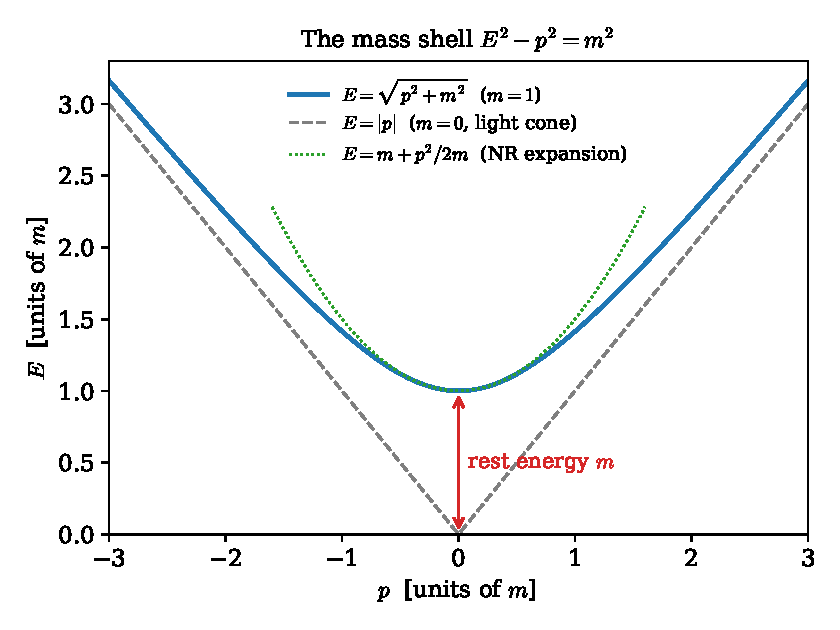
\includegraphics[width=0.68\textwidth]{fig_mass_shell.pdf}
  \caption{The mass shell \eqref{eq:mass-shell} in $1{+}1$ momentum
  space: the exact relativistic dispersion (blue), its massless
  light-cone asymptote (gray, dashed), and the nonrelativistic
  parabola $E = m + p^2/2m$ of Eq.~\eqref{eq:energy-expansion}
  (green, dotted), which hugs the shell near $p = 0$ and departs
  from it at large $p$. This figure returns, with the axes relabeled
  $(\omega, k)$, as the Klein--Gordon dispersion relation in
  \S\ref{sec:klein-gordon}.}
  \label{fig:mass-shell}
\end{figure}

\begin{example}[LHC protons: the worked number]\label{ex:lhc}
An LHC beam proton has $E = 6.8\,\mathrm{TeV}$ and
$m = 0.938\,\mathrm{GeV}$, so
\begin{equation}
  \gamma = \frac{E}{m} = 7.25\times 10^{3},
  \qquad
  1 - \beta \approx \frac{1}{2\gamma^2} = 9.5\times 10^{-9} :
\end{equation}
the proton trails a light pulse by about
$c\,(1-\beta) \approx 2.9\,\mathrm{m/s}$ --- walking pace --- while
carrying $7250$ times its rest energy. On Fig.~\ref{fig:mass-shell} it
sits far up the asymptote, where the shell and the light cone are
indistinguishable to one part in $10^8$.
\end{example}

\begin{remark}[The other six charges]\label{rem:ten-charges}
Section~\ref{sec:lorentz-group} promised ten conservation laws for the
ten Poincar\'e parameters; translations have now supplied four. The three
rotations conserve angular momentum $\vec L = \vx \times \vp$, exactly
as in [Mech.\ \S3.3] --- nothing relativistic changes in that
derivation. The three boosts conserve the less famous
$\vec K = E\,\vx - t\,\vp$: indeed
$\dd\vec K/\dd t = E\vv - \vp - t\,\dot{\vp} = \gamma m \vv - \gamma m
\vv - 0 = 0$. Solving $\vec K = \mathrm{const}$ for $\vx$ shows its
meaning: the point $\vx = (\vec K + t\vp)/E$ --- the center of energy
--- moves uniformly. Boost symmetry conserves the \emph{uniformity of
the center-of-energy motion}, the relativistic upgrade of the
center-of-mass theorem. All six reappear, localized into densities,
in \S\ref{sec:noether-fields}.
\end{remark}

\subsection{The relativistic Hamiltonian}
\label{sec:particle-hamiltonian}

The Legendre transform [Mech.\ \S6] completes the particle's
description. Invert \eqref{eq:canonical-momentum} for the velocity: squaring,
$|\vp|^2 (1 - v^2) = m^2 v^2$ gives
\begin{equation}
  \vv = \frac{\vp}{\sqrt{|\vp|^2 + m^2}},
\end{equation}
and the Hamiltonian is
\begin{equation}
  H(\vp)
  = \vp \cdot \vv - L
  = \frac{|\vp|^2}{\sqrt{|\vp|^2+m^2}}
    + \frac{m^2}{\sqrt{|\vp|^2+m^2}}
  \;=\;
  \boxed{\ \sqrt{|\vp|^2 + m^2}\ }
  \label{eq:relativistic-hamiltonian}
\end{equation}
--- the mass-shell function itself, as it must be: $L$ has no explicit
time dependence, so $H$ equals the conserved energy
[Mech.\ \S6.3], and the conserved energy \eqref{eq:energy} lives on
the shell \eqref{eq:mass-shell}. Hamilton's equations close the loop:
\begin{equation}
  \dot{\vx} = \pd{H}{\vp} = \frac{\vp}{\sqrt{|\vp|^2+m^2}} = \vv,
  \qquad
  \dot{\vp} = -\pd{H}{\vx} = 0 .
\end{equation}

\begin{remark}[Is $H$ covariant? No --- and instructively so]
\label{rem:H-not-covariant}
Route 2 delivered the manifestly covariant
Eq.~\eqref{eq:covariant-eom}; the Hamiltonian route cannot deliver its
like, and the loss happens at the first step: the Legendre transform
differentiates with respect to \emph{somebody's} time, so writing a
Hamiltonian means choosing a slicing of spacetime into moments. Nor is
$H$ itself a scalar --- it is the \emph{time component} of $p^\mu$,
so different inertial observers use different Hamiltonians, related by
boosts. Covariance is not broken, but it is demoted from a property
visible by inspection to a theorem requiring proof: the ten charges of
Remark~\ref{rem:ten-charges} must close, under Poisson brackets, into
the algebra of the Poincar\'e group. In that algebra $H$ and $\vec K$
are the generators that \emph{move the time slice}, and the fact that
they do not commute is already on display:
$\vec K = E\vx - t\vp$ carries explicit time dependence, and its
conservation is a cancellation,
\begin{equation}
  \tot{K_i}{t}
  = \pd{K_i}{t} + \{K_i, H\}
  = -\,p_i + E\,\pd{H}{p_i}
  = -\,p_i + p_i = 0,
\end{equation}
with $\{K_i, H\} = p_i \neq 0$ --- the classical fingerprint of the
commutator $[\hat K_i, \hat H] \neq 0$ that canonical quantum field
theory must live with. The same trade returns at field level in
\S\ref{sec:hamiltonian-fields}: there $H = \int T^{00}\,\dd^3x$ is
again a $00$-component integrated over a chosen slice, canonical
quantization inherits the non-manifest covariance, and ``the quantum
theory is Lorentz invariant'' becomes a statement about the algebra of
operator charges, verified rather than seen. (A manifestly covariant
Hamiltonian formulation of the particle does exist: take the worldline
parameter itself as time, whereupon $H$ vanishes identically and the
dynamics hides inside the constraint $p \cdot p = m^2$ --- the
Hamiltonian face of Remark~\ref{rem:reparametrization}'s
reparametrization redundancy. Constrained-dynamics territory;
deferred. [stated.])
\end{remark}

\begin{remark}[The square-root problem]
\label{rem:square-root}
$H = \sqrt{|\vp|^2 + m^2}$ is an unpleasant object to promote to a
quantum operator: the square root of a differential operator is
nonlocal, and awkward to work with. The historical escape
was to \emph{square} the relation --- demand
$E^2 = |\vp|^2 + m^2$ of a wave $\ee^{-\ii(Et - \vp\cdot\vx)}$ ---
which yields not a Schr\"odinger-type equation but the
\emph{Klein--Gordon equation}, a field equation. That road, from the
awkward square root to relativistic fields, is exactly the road this
document travels: \S\ref{sec:klein-gordon} arrives at Klein--Gordon
from the Lagrangian side, and Fig.~\ref{fig:mass-shell} will be
waiting there with its axes relabeled.
\end{remark}

%=======================================================================
\section{The Charged Particle}
%=======================================================================
\label{sec:charged-particle}

The free particle exhausted what a bare worldline can do. To make
anything else happen, the particle needs an environment --- and the
simplest relativistic environment is a four-vector field
$A_\mu(x)$ defined over spacetime, coupled in the simplest way the
covariance principle permits. This short section builds that coupling,
finds that its redundancy and its equation of motion are both familiar
--- gauge freedom and the Lorentz force ---
and establishes two structures that Part III will need: the antisymmetric
derivative combination $F_{\mu\nu}$, and the split between canonical
and mechanical momentum.

\subsection{The coupling}
\label{sec:coupling}

What scalar can be built that is \emph{linear} in a vector field
$A_\mu$ and local to the worldline? The field must be evaluated on the
worldline and contracted with something the worldline provides; the
worldline provides $\dd x^\mu$. Hence, appended to the free action
\eqref{eq:particle-action}:
\begin{equation}
  \boxed{\;
  S \;=\; -\,m \int \dd\tau
  \;-\; q \int A_\mu(x)\,\dd x^\mu ,
  \;}
  \label{eq:charged-action}
\end{equation}
with a coupling constant $q$ --- the \emph{charge} --- measuring how
strongly this particular particle couples to this particular field.
The interaction term is a Lorentz scalar by construction (one upper
index contracted against one lower), and it is reparametrization invariant without
help: $\dd x^\mu$ needs no $\dd\tau$, no metric, no clock. To
recognize it, parametrize by lab time. With the traditional names for
the components, $A^\mu = (\varphi, \vec A)$ --- so
$A_\mu = (\varphi, -\vec A)$ --- the integrand is
$A_\mu \dd x^\mu = \varphi\,\dd t - \vec A \cdot \dd\vx$, and
\begin{equation}
  L = -\,m\sqrt{1 - v^2}
      \;-\; q\,\varphi(t, \vx)
      \;+\; q\,\vec A(t, \vx) \cdot \vv .
  \label{eq:charged-lagrangian}
\end{equation}
The scalar potential enters like a potential energy; the vector
potential enters through a velocity-dependent term --- the first
Lagrangian of the series in which force will depend on velocity.

\subsection{Gauge invariance of the coupling}
\label{sec:gauge-coupling}

The field $A_\mu$ enters \eqref{eq:charged-action} with a redundancy.
Shift it by the four-gradient of any scalar function:
\begin{equation}
  \boxed{\;
  A_\mu \;\longrightarrow\; A_\mu + \partial_\mu \chi .
  \;}
  \label{eq:gauge-transformation}
\end{equation}
The interaction changes by
\begin{equation}
  -\,q \int \partial_\mu \chi\;\dd x^\mu
  = -\,q \int \dd\chi
  = -\,q\,\bigl[\chi(x_B) - \chi(x_A)\bigr]
\end{equation}
--- a pure endpoint term, which variations with pinned endpoints never
see [Mech.\ \S2.2]. Every choice of $\chi$ yields the \emph{same}
equations of motion: the four functions $A_\mu$ overdescribe the
physics, and the overdescription is exactly one scalar function's
worth. This is the pattern of Remark~\ref{rem:reparametrization}
in mirror image --- there, redundancy in the
\emph{worldline's} description produced an empty equation; here, the
redundancy sits in the \emph{background's} description. What the equations
of motion can depend on is only the gauge-invariant content of
$A_\mu$, and the next subsection watches the variational principle
extract precisely that content on its own.

\subsection{Equations of motion: the Lorentz force}
\label{sec:lorentz-force}

\paragraph{Route 1: lab coordinates.}
Run Euler--Lagrange on \eqref{eq:charged-lagrangian}. The canonical
momentum picks up a field contribution:
\begin{equation}
  \boxed{\;
  \vec P \;\equiv\; \pd{L}{\vv}
  \;=\; \gamma m \vv + q \vec A
  \;=\; \vp + q\vec A,
  \;}
  \label{eq:canonical-vs-mechanical}
\end{equation}
where $\vp = \gamma m \vv$ is the \emph{mechanical} momentum of
\eqref{eq:canonical-momentum} --- the distinction matters and returns
in \S\ref{sec:canonical-mechanical}. The coordinate derivative of $L$:
\begin{equation}
  \pd{L}{\vx}
  = -\,q\nabla\varphi + q\,\nabla(\vec A \cdot \vv),
\end{equation}
the gradient acting on the field arguments only ($\vv$ is an
independent slot of the Lagrangian, not a field on space). The
Euler--Lagrange equation
$\dd\vec P/\dd t = \partial L/\partial\vx$ needs the total time
derivative of $\vec A$ \emph{along the moving particle}, which is the
convective derivative:
\begin{equation}
  \tot{\vec A}{t}
  = \pd{\vec A}{t} + (\vv \cdot \nabla)\vec A
\end{equation}
--- the particle feels the field change both because the field changes
and because the particle moves through it. Assembling:
\begin{equation}
  \tot{\vp}{t}
  = -\,q\left(\nabla\varphi + \pd{\vec A}{t}\right)
    + q\,\Bigl[\nabla(\vec A \cdot \vv) - (\vv\cdot\nabla)\vec A\Bigr].
  \label{eq:force-raw}
\end{equation}
The last bracket is the curl identity
$\vv \times (\nabla \times \vec A) =
\nabla(\vec A\cdot\vv) - (\vv\cdot\nabla)\vec A$ (valid because $\vv$
carries no position dependence). The equation of motion has organized
its right side into two derivative combinations of the potentials, and
we \emph{name} them:
\begin{equation}
  \vE \;\equiv\; -\nabla\varphi - \pd{\vec A}{t},
  \qquad
  \vB \;\equiv\; \nabla \times \vec A ,
  \label{eq:E-B-definitions}
\end{equation}
whereupon
\begin{equation}
  \boxed{\;
  \tot{}{t}\bigl(\gamma m \vv\bigr)
  \;=\; q\,\bigl(\vE + \vv \times \vB\bigr) :
  \;}
  \label{eq:lorentz-force}
\end{equation}
the Lorentz force law, derived rather than postulated. Two things deserve to be said
about the derivation rather than the result. First, $\vE$ and $\vB$
were not inputs: they are the combinations of potential derivatives
that the variational principle assembled on its own, and both are
inert under the gauge shift \eqref{eq:gauge-transformation} ---
$\nabla \times \nabla\chi = 0$ kills it in $\vB$, and
$-\nabla\dot\chi - \partial_t\nabla\chi = 0$ in $\vE$ --- exactly as
\S\ref{sec:gauge-coupling} predicted the equations of motion must
arrange. Second, the left side is the \emph{mechanical} momentum: what
the force pushes is $\gamma m\vv$, not the canonical $\vec P$.

\paragraph{Route 2: covariant form.}
The same variation without choosing a frame produces the central
object of Part III. Vary the interaction in worldline form,
$S_{\text{int}} = -q\int A_\mu(x)\,\dot x^\mu\,\dd\lambda$:
\begin{align}
  \delta S_{\text{int}}
  &= -\,q \int \Bigl[
      \bigl(\partial_\nu A_\mu\bigr)\,\delta x^\nu\, \dot x^\mu
      + A_\nu\, \delta\dot x^\nu
    \Bigr] \dd\lambda
  \notag\\
  &= -\,q \int \Bigl[
      \partial_\nu A_\mu\,\dot x^\mu
      - \tot{}{\lambda}A_\nu
    \Bigr]\,\delta x^\nu\, \dd\lambda
  = -\,q \int \Bigl[
      \partial_\nu A_\mu - \partial_\mu A_\nu
    \Bigr]\,\dot x^\mu\,\delta x^\nu\, \dd\lambda ,
\end{align}
integrating by parts in the second step and using
$\dd A_\nu/\dd\lambda = \dot x^\mu \partial_\mu A_\nu$ (the covariant
convective derivative) in the third. Adding the free variation from
\S\ref{sec:particle-eom} and demanding stationarity:
\begin{equation}
  \boxed{\;
  m\,\tot{u^\mu}{\tau} \;=\; q\, F^\mu{}_\nu\, u^\nu,
  \qquad
  F_{\mu\nu} \;\equiv\; \partial_\mu A_\nu - \partial_\nu A_\mu .
  \;}
  \label{eq:covariant-lorentz-force}
\end{equation}
The variation \emph{manufactured} the antisymmetric combination
$F_{\mu\nu}$ --- the only part of $\partial_\mu A_\nu$ that survives,
and manifestly gauge invariant, since
$\partial_\mu\partial_\nu\chi - \partial_\nu\partial_\mu\chi = 0$.
And its tensor character comes with no extra work: the force
\eqref{eq:covariant-lorentz-force} is linear in the four-vector
$u^\nu$ with a four-vector result, so by the quotient rule
(Proposition~\ref{prop:quotient}) $F^\mu{}_\nu$ \emph{is} a
$(1,1)$ tensor --- as promised in \S\ref{sec:tensors}. Its
six independent components (antisymmetry kills the diagonal and
pairs the rest) are exactly the six numbers
\eqref{eq:E-B-definitions}: $\vE$ and $\vB$ are one tensor seen in
$3+1$ pieces, which Part III displays in full
(\S\ref{sec:field-tensor}).

\begin{example}[The LHC proton, bent: the worked number]
\label{ex:lhc-bending}
For circular motion at constant speed, $\gamma$ is constant, and
\eqref{eq:lorentz-force} in a pure magnetic field reads
$\gamma m\,v^2/r = qvB$, so
\begin{equation}
  r = \frac{\gamma m v}{qB} = \frac{p}{qB} :
\end{equation}
the bending radius is set by the \emph{mechanical momentum}, $\gamma$
included. The proton of Example~\ref{ex:lhc}
($p \approx E = 6.8\,\mathrm{TeV}$) rides a dipole field
$B = 8.1\,\mathrm{T}$ (the magnets' $8.33\,\mathrm{T}$ design value
scaled to the running energy), so
\begin{equation}
  r = \frac{6800\,\mathrm{GeV}}{0.300 \times 8.1\,\mathrm{T}}
      \,\mathrm{\frac{m}{GeV/T}}
    \approx 2.80\,\mathrm{km},
\end{equation}
the machine's actual bending radius. The cyclotron frequency
$\omega = qB/(\gamma m)$ falls with energy --- which is why a
fixed-frequency cyclotron fails relativistically and the LHC is a
\emph{synchro}tron, its fields ramped in step with $\gamma$.
\end{example}

\begin{example}[Constant field: hyperbolic motion]\label{ex:hyperbolic}
The simplest exact solution of \eqref{eq:covariant-lorentz-force}: a
uniform, static $\vE = E\,\hat x$, no $\vB$, charge starting from rest.
The potentials $\varphi = -Ex$, $\vec A = 0$ give (check against
\eqref{eq:E-B-definitions}: $-\nabla\varphi = E\hat x$) the single
nonzero pair
$F_{01} = \partial_0 A_1 - \partial_1 A_0 = E$, whence
$F^0{}_1 = \eta^{00}F_{01} = E$ and
$F^1{}_0 = \eta^{11}F_{10} = E$. The covariant force law reduces to
two coupled components, with $\alpha \equiv qE/m$:
\begin{equation}
  \tot{u^0}{\tau} = \alpha\, u^1,
  \qquad
  \tot{u^1}{\tau} = \alpha\, u^0
  \qquad\Longrightarrow\qquad
  \tot{}{\tau}\bigl(u^0 \pm u^1\bigr) = \pm\,\alpha\,\bigl(u^0 \pm u^1\bigr):
\end{equation}
the \emph{null combinations} of \S\ref{sec:lorentz-derivation}
diagonalize the dynamics exactly as they diagonalized the boost.
Starting from rest, $u^\mu(0) = (1, 0)$, so $u^0 \pm u^1 =
\ee^{\pm\alpha\tau}$ and
\begin{equation}
  u^0 = \cosh\alpha\tau,
  \qquad
  u^1 = \sinh\alpha\tau :
\end{equation}
the \emph{rapidity grows linearly in proper time}, $\phi = \alpha\tau$
--- each proper second adds the same rapidity increment, and
$\beta = \tanh\phi$ approaches but never reaches $1$, which is
Remark~\ref{rem:sanity}(iii) in dynamical form. Integrating once more,
\begin{equation}
  t = \alpha^{-1}\sinh\alpha\tau,
  \qquad
  x = \alpha^{-1}\bigl(\cosh\alpha\tau - 1\bigr)
  \qquad\Longrightarrow\qquad
  \bigl(x + \alpha^{-1}\bigr)^2 - t^2 = \alpha^{-2} :
\end{equation}
the worldline is one of the calibration hyperbolae of
Fig.~\ref{fig:hyperbolae} --- hence \emph{hyperbolic motion}. The
four-acceleration $a^\mu = \dd u^\mu/\dd\tau =
\alpha\,(\sinh\alpha\tau,\, \cosh\alpha\tau)$ satisfies $a \cdot u = 0$
by inspection and has constant invariant norm
$\sqrt{-a\cdot a} = \alpha = qE/m$: constant \emph{proper}
acceleration --- the higher-derivative scalar mentioned in
\S\ref{sec:particle-action}, realized here by the simplest field. One
number, units restored: at proper acceleration $g$, one year of proper
time gives $\phi = g\tau/c \approx 1.03$, hence $\beta \approx 0.77$,
with about $1.19$ years of coordinate time elapsed and $0.56$
light-years covered.
\end{example}

\subsection{Canonical versus mechanical momentum}
\label{sec:canonical-mechanical}

Equation \eqref{eq:canonical-vs-mechanical} split the momentum in two,
and the two halves divide the labor:
\begin{center}
\begin{tabular}{lll}
\toprule
 & mechanical $\vp = \gamma m\vv$ & canonical $\vec P = \vp + q\vec A$ \\
\midrule
gauge behavior & invariant & shifts by $q\nabla\chi$ \\
what force acts on & Eq.~\eqref{eq:lorentz-force} & --- \\
Noether charge of $\vx \to \vx + \vec\epsilon$ & --- & conserved (when $A_\mu$ is $\vx$-independent) \\
enters Hamilton's equations & --- & $\vec P$ is the phase-space variable \\
\bottomrule
\end{tabular}
\end{center}
Neither column can do the other's job: the measurable, gauge-invariant
$\vp$ is not the conserved quantity; the conserved $\vec P$ is not
gauge invariant, and by itself not measurable. The Hamiltonian makes
the division explicit. Legendre-transforming
\eqref{eq:charged-lagrangian} with respect to $\vec P$ (the inversion
runs exactly as in \S\ref{sec:particle-hamiltonian} with
$\vp = \vec P - q\vec A$):
\begin{equation}
  \boxed{\;
  H(\vx, \vec P)
  = \sqrt{\,\bigl(\vec P - q\vec A\bigr)^2 + m^2\,}
    \;+\; q\,\varphi .
  \;}
  \label{eq:minimal-coupling}
\end{equation}
Comparing with the free
$H = \sqrt{|\vec P|^2 + m^2}$: the entire interaction is the
substitution
\begin{equation}
  \vec P \to \vec P - q\vec A,
  \qquad
  H \to H - q\varphi
  \qquad\text{i.e.}\qquad
  p^\mu \;\to\; p^\mu - qA^\mu
  \label{eq:minimal-substitution}
\end{equation}
--- \emph{minimal coupling}, the rule quantum mechanics will inherit
verbatim ($\hat{\vec p} \to \hat{\vec p} - q\vec A$ in the Pauli and
Dirac equations) and quantum field theory will re-derive from gauge
symmetry. That the whole of electromagnetism's action on matter
compresses into one substitution is not an accident of this
Lagrangian; it is the classical shadow of the gauge principle, and the
outlook (\S\ref{sec:outlook}) says one more word about it.

\medskip
\noindent
Part I is complete: kinematics from two postulates, dynamics from one
scalar action, energy and momentum from Noether, and a first field ---
entering as a fixed background to which the particle couples. The
obvious next question is the reverse one: what
dynamics does $A_\mu$ itself obey, and what action prescribes it?
Answering requires learning to vary \emph{fields} rather than
worldlines, and that is Part II's business --- built, like everything
in this series, from a chain of masses.

%=======================================================================
\clearpage
\part{Classical Field Theory}
%=======================================================================

%=======================================================================
\section{From Chain to Field}
%=======================================================================
\label{sec:chain-to-field}

Part I closed by asking for the dynamics of a field. This section
builds the concept from the series' oldest object: the bead chain
of [Osc.\ \S8--9]. There, the continuum limit was taken in the
\emph{equations of motion} --- a limit in each equation. Here
it is taken once, in the \emph{Lagrangian}, and the single limit does
more than reproduce the wave equation: it exposes the structural pivot
on which all of field theory turns --- the demotion of position from
dynamical variable to label.

\subsection{The chain acquires a Lagrangian}
\label{sec:chain-lagrangian}

Recall the setting of [Osc.\ \S9.1]: $N$ beads of mass $m$, spaced $a$
apart on a massless string under tension $T$ between fixed walls, with
small transverse displacements $y_j(t)$, $j = 1, \dots, N$ (and
$y_0 = y_{N+1} = 0$ at the walls). There, Newton delivered
\begin{equation}
  m\ddot y_j = \frac{T}{a}\bigl(y_{j-1} - 2y_j + y_{j+1}\bigr).
  \label{eq:bead-eom}
\end{equation}
The Lagrangian route needs the one ingredient the free-body diagram
never wrote down: the potential energy. It is the work done against
tension by the \emph{extra length} of the displaced string. The
segment from bead $j$ to bead $j+1$ has length
\begin{equation}
  \sqrt{a^2 + (y_{j+1}-y_j)^2}
  = a\,\sqrt{1 + \Bigl(\tfrac{y_{j+1}-y_j}{a}\Bigr)^{\!2}}
  = a + \frac{(y_{j+1}-y_j)^2}{2a} + O\bigl((\Delta y)^4\bigr),
\end{equation}
so, to the same small-slope order as \eqref{eq:bead-eom},
\begin{equation}
  U = T \times (\text{excess length})
    = \sum_{j=0}^{N} \frac{T}{2a}\,\bigl(y_{j+1}-y_j\bigr)^2 ,
  \qquad
  L = \sum_{j=1}^{N} \tfrac12\, m\,\dot y_j^{\,2}
    \;-\; \sum_{j=0}^{N} \frac{T}{2a}\,\bigl(y_{j+1}-y_j\bigr)^2 .
  \label{eq:chain-lagrangian}
\end{equation}
Check against \eqref{eq:bead-eom}: the coordinate $y_j$ appears in
\emph{two} terms of the potential sum --- the spring on its left and
the spring on its right ---
\begin{equation}
  \pd{L}{y_j}
  = -\frac{T}{a}\Bigl[
      \bigl(y_j - y_{j-1}\bigr) - \bigl(y_{j+1} - y_j\bigr)
    \Bigr]
  = \frac{T}{a}\bigl(y_{j-1} - 2y_j + y_{j+1}\bigr),
  \label{eq:two-neighbors}
\end{equation}
and Euler--Lagrange, $\dd(\partial L/\partial\dot y_j)/\dd t =
\partial L/\partial y_j$, reproduces \eqref{eq:bead-eom} exactly. Note
for later the mechanism of \eqref{eq:two-neighbors}: differencing with
\emph{both} neighbors is what turned one difference into a second
difference. It is the discrete shadow of an integration by parts, and
\S\ref{sec:field-variational} meets its continuum original.

\subsection{Taking the limit once}
\label{sec:limit-once}

Refine as in [Osc.\ \S9.2]: $a \to 0$, $N \to \infty$, holding fixed
the physical rope --- its length $L_{\text{rope}} = (N+1)a$, its mass
per length $\mu = m/a$, and its tension $T$. The displacements merge
into a smooth profile, and here is the moment the notation should mark:
write
\begin{equation}
  y_j(t) \;=\; \phi(x_j, t),
  \qquad x_j = ja,
\end{equation}
renaming $y \to \phi$ as the displacement sheds its origin (a
transverse direction) and becomes an abstract \emph{field value} ---
the letter $\phi$ serves for the rest of the document, and no
confusion with the rapidity survives §\ref{sec:minkowski}'s $c=1$
switch. Then $\dot y_j = \dot\phi(x_j, t)$ and
$(y_{j+1} - y_j)/a \to \partial\phi/\partial x \equiv \phi'$, and the
Lagrangian \eqref{eq:chain-lagrangian}, rewritten to expose one factor
of $a$ per term,
\begin{equation}
  L = \sum_{j} a \left[
    \frac12\,\frac{m}{a}\,\dot y_j^{\,2}
    - \frac12\,T \Bigl(\frac{y_{j+1}-y_j}{a}\Bigr)^{\!2}
  \right],
\end{equation}
converges as a Riemann sum, $\sum_j a \to \int \dd x$, to
\begin{equation}
  \boxed{\;
  L = \int_0^{L_{\text{rope}}} \dd x\;
      \mathcal L\bigl(\dot\phi, \phi'\bigr),
  \qquad
  \mathcal L
  = \tfrac12\,\mu\,\dot\phi^{\,2}
  - \tfrac12\,T\,\phi'^{\,2} .
  \;}
  \label{eq:string-lagrangian-density}
\end{equation}
$\mathcal L$ is the \emph{Lagrangian density} --- Lagrangian per unit
length --- and its two terms are exactly the kinetic and potential
energy densities of the rope. One limit, taken in one object; the
equations of motion will be extracted from it once, for all $x$
simultaneously, in \S\ref{sec:field-variational}.

\begin{figure}[htbp]
  \centering
  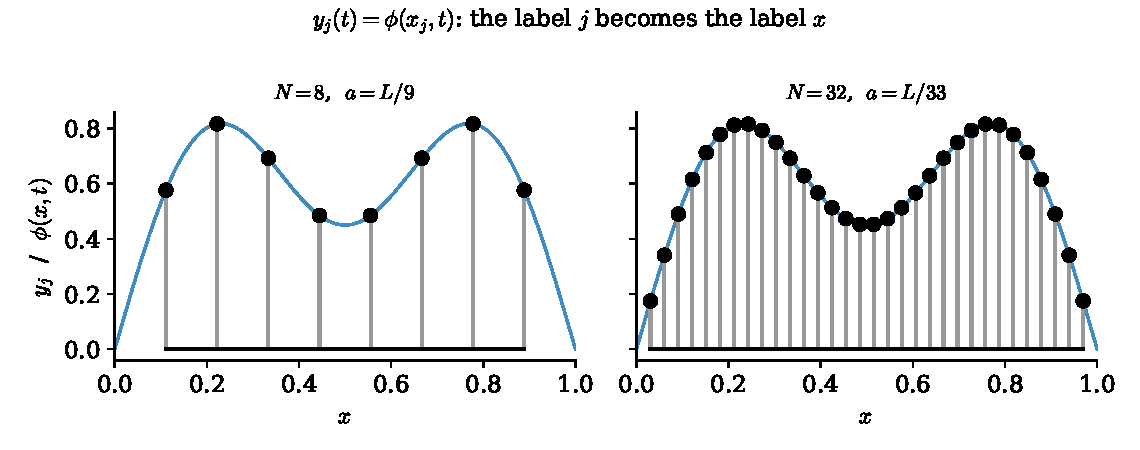
\includegraphics[width=0.95\textwidth]{fig_chain_to_field.pdf}
  \caption{The same smooth profile sampled by two chains
  ($N = 8$ and $N = 32$ beads). The dynamical variables are the
  heights $y_j$; the site index $j$ --- equivalently the position
  $x_j = ja$ --- merely \emph{labels} them. Refining the chain makes
  the label continuous and the collection of heights a function
  $\phi(x, t)$; nothing about the label's role changes.}
  \label{fig:chain-to-field}
\end{figure}

\subsection{The pivot: $x$ is demoted from variable to label}
\label{sec:pivot}

Now look at what happened to the letter $x$ --- the point of the whole
construction, easy to use forever without once being said aloud.

In mechanics, position is what the theory is \emph{about}: the
$q_i(t)$ are the dynamical variables, and $t$ is the label
parametrizing their evolution. In \eqref{eq:string-lagrangian-density}
the dynamical variable is $\phi$ --- the field's \emph{value} --- and
$x$ stands beside $t$ as a second label, saying \emph{which} degree of
freedom is meant, exactly as the index $j$ did on the chain
(Fig.~\ref{fig:chain-to-field}). The chain makes the demotion
undramatic: $j$ was never a dynamical variable, and $x_j = ja$ is just
$j$ wearing units. A field theory is a mechanical system with a
continuous infinity of degrees of freedom, one per point of space, and
the whole translation is a dictionary:

\begin{center}
\begin{tabular}{lll}
\toprule
 & mechanics / chain & field theory \\
\midrule
labels degrees of freedom & index $i$ & position $x$ \\
dynamical variable & $q_i(t)$ & $\phi(x, t)$ \\
aggregation & $\displaystyle\sum_i$ & $\displaystyle\int \dd x$ \\
Lagrangian & $L(q, \dot q)$ & $L = \displaystyle\int \dd x\;\mathcal L(\phi, \dot\phi, \phi')$ \\
sensitivity to one d.o.f. & $\displaystyle\pd{L}{q_i}$ & $\displaystyle\frac{\delta L}{\delta\phi(x)}$ \quad(\S\ref{sec:field-variational}) \\
coupling structure & matrix $\mathsf K_{ij}$ (near-diagonal) & differential operator $-T\,\partial_x^2$ (local) \\
normal modes & eigenvectors of $\mathsf K$ [Osc.\ \S8] & Fourier modes \\
\bottomrule
\end{tabular}
\end{center}

\noindent
Two of the rows remain to be justified. The functional derivative
$\delta L/\delta\phi(x)$ --- ``the partial derivative of $L$ with
respect to the single degree of freedom sitting at $x$'' --- is
defined properly in \S\ref{sec:field-variational}. And the mode row is
already verified: [Osc.\ \S9.3] showed the chain's normal modes turning
into the string's Fourier modes, with the dispersion
$\omega = 2\sqrt{T/(ma)}\,\sin(ka/2)$ flattening to
$\omega = c_s k$, $c_s^2 = T/\mu$, as $ka \to 0$ --- the dictionary's
last row, verified before the dictionary existed.

\begin{remark}[Why relativity insists on fields]
\label{rem:relativity-insists}
Part I gives the pivot a second, independent motivation. Under a
boost, $t$ and $x$ mix (Theorem~\ref{thm:lorentz}); but mechanics
hardwires an asymmetry between them --- $t$ a label, position a
dynamical variable --- so a mechanics of particles can be made
relativistic only against the grain (the covariant formalism of
\S\ref{sec:relativistic-particle} had to demote $t$ itself to a
function $x^0(\lambda)$ of an unphysical label to restore the
symmetry, and Remark~\ref{rem:reparametrization} was the consequence). Field
theory dissolves the asymmetry at the root: $t$ and $x$ sit on the
same side of the dictionary, joint labels $x^\mu$ on one dynamical
variable $\phi$, and Lorentz transformations act on labels exactly as
\S\ref{sec:tensors}'s tensor fields require. The string itself is not
relativistic --- its $c_s = \sqrt{T/\mu}$ is no invariant speed, and
\S\ref{sec:wave-revisited}'s conclusion stands --- but the \emph{shape}
of its description is precisely the shape relativistic dynamics needs,
which is why \S\ref{sec:klein-gordon} will need to change almost
nothing.
\end{remark}

\noindent
The Lagrangian \eqref{eq:string-lagrangian-density} is in hand and the
question it raises is sharp: $L$ now takes a whole function
$\phi(\cdot, t)$ at each instant --- it is a \emph{functional}, in
exactly the sense of [Mech.\ \S1] --- so what replaces
$\partial L/\partial q_i$, and what do its Euler--Lagrange equations
look like? That is the next section, and the machinery is already
built: the Gateaux framework of [Mech.\ \S2.2] was designed for
functionals and does not care that this one's argument is a field.

%=======================================================================
\section{The Field Variational Principle}
%=======================================================================
\label{sec:field-variational}

The Lagrangian \eqref{eq:string-lagrangian-density} takes a function and
returns a number; its time integral, the action, is therefore a
functional of the field's whole history. Extracting equations of
motion from such an object is exactly the problem [Mech.\ \S2] solved
--- the only novelty is that the ``curve'' being varied is now a
function of \emph{two} labels, and the variation will integrate by
parts in both. This section runs the machinery once for a general
density, supplies the functional derivative the dictionary promised, gives
boundary terms the separate treatment they deserve, and closes two
threads: the wave equation (a third time) and the fate of the string's
accidental Lorentz invariance.

\subsection{Hamilton's principle for fields}
\label{sec:hamilton-fields}

Let the density depend on the field's value and first derivatives ---
general enough for everything in this document:
\begin{equation}
  S[\phi]
  = \int_{t_1}^{t_2}\!\dd t \int_0^{\ell}\!\dd x\;
    \mathcal L\bigl(\phi,\, \dot\phi,\, \phi'\bigr),
  \label{eq:field-action}
\end{equation}
(writing $\ell$ for the spatial extent; the infinite line is the limit
$\ell \to \infty$ with decay conditions, \S\ref{sec:boundary-terms}).
Hamilton's principle,\footnote{A terminological trap worth disarming
once: Hamilton's principle, $\delta\!\int\! L\,\dd t = 0$, is the
variational principle \emph{of Lagrangian mechanics} --- the name
honors its author (Hamilton, 1834--35), not the function varied.
Lagrange himself derived his equations from d'Alembert's principle of
virtual work [Mech.\ \S3.2], with no action functional in sight;
Hamilton's name thus sits on both sides of the Legendre transform ---
this principle on the Lagrangian side, Hamilton's equations on the
other --- by biographical accident. The alternative name ``principle
of least action'' is worse: historically it denotes Maupertuis'
principle (fixed energy, free transit time, abbreviated action
$\int \vp\cdot\dd\vec q$), a genuinely different variational statement.}
verbatim from [Mech.\ \S3.1]: \emph{the physical
field history makes $S$ stationary} among histories with prescribed
field configurations at $t_1$ and $t_2$ and prescribed spatial
boundary behavior.

Vary in the Gateaux sense of [Mech.\ \S2.2]:
$\phi \to \phi + \varepsilon\,\eta(x,t)$ with $\eta(x, t_1) =
\eta(x, t_2) = 0$, and
\begin{equation}
  \delta S[\phi;\eta]
  = \left.\tot{}{\varepsilon}\right|_{0} S[\phi + \varepsilon\eta]
  = \int\!\!\int \dd t\,\dd x
    \left[
      \pd{\mathcal L}{\phi}\,\eta
      + \pd{\mathcal L}{\dot\phi}\,\dot\eta
      + \pd{\mathcal L}{\phi'}\,\eta'
    \right],
  \label{eq:field-first-variation}
\end{equation}
by the chain rule, with the slot-derivative shorthand of
[Mech.\ \S2.2]. Two integrations by parts free $\eta$ --- one in $t$
per term two, one in $x$ per term three:
\begin{equation}
  \delta S
  = \int\!\!\int \dd t\,\dd x
    \left[
      \pd{\mathcal L}{\phi}
      - \pd{}{t}\!\left(\pd{\mathcal L}{\dot\phi}\right)
      - \pd{}{x}\!\left(\pd{\mathcal L}{\phi'}\right)
    \right] \eta
  \;+\;
  \int_{t_1}^{t_2}\!\dd t
    \left[\pd{\mathcal L}{\phi'}\,\eta\right]_{x=0}^{x=\ell}.
  \label{eq:field-variation-ibp}
\end{equation}
The temporal boundary term died on the pinned endpoints, as always;
the \emph{spatial} boundary term is new, and care keeps
it visible --- \S\ref{sec:boundary-terms} is devoted to the ways it
vanishes. Granting that it does: $\eta$ is arbitrary in the interior,
the fundamental lemma applies (its proof [Mech.\ App.\ B] extends to
two integration variables with only notational changes --- choose the
bump function as a product of two one-variable bumps [stated; the
one-line adaptation is left to the reader]), and:

\begin{theorem}[Field Euler--Lagrange equation]\label{thm:field-EL}
A field history making \eqref{eq:field-action} stationary, with
vanishing spatial boundary term, satisfies
\begin{equation}
  \boxed{\;
  \pd{}{t}\!\left(\pd{\mathcal L}{\dot\phi}\right)
  + \pd{}{x}\!\left(\pd{\mathcal L}{\phi'}\right)
  - \pd{\mathcal L}{\phi}
  = 0
  \qquad \text{at every } (x, t).
  \;}
  \label{eq:field-EL}
\end{equation}
\end{theorem}

\noindent
Set beside its ancestor
$\dd(\partial L/\partial\dot q)/\dd t - \partial L/\partial q = 0$:
the only change is that the label $x$, having joined $t$ in the
dictionary of \S\ref{sec:pivot}, now also supplies a derivative term
--- one term per label, symmetrically, a symmetry \S\ref{sec:klein-gordon}
will make manifest. And the promised reunion: the spatial integration
by parts that produced the $\partial_x(\partial\mathcal L/\partial\phi')$
term is the continuum original of the two-neighbor mechanism of
Eq.~\eqref{eq:two-neighbors} --- there, $y_j$ sat in two springs and
the two first differences assembled a second difference; here, $\phi(x)$
sits under one derivative and the integration by parts moves it,
signs and all, to the same effect.

\subsection{Defining the functional derivative}
\label{sec:functional-derivative}

Section~\ref{sec:pivot} promised a meaning for
$\delta L/\delta\phi(x)$ --- ``the sensitivity of $L$ to the single
degree of freedom at $x$.'' The Gateaux variation supplies it. For the
fixed-time functional $L[\phi] = \int\dd x\,
\mathcal L(\phi, \dot\phi, \phi')$, collect the variation (spatial
boundary term disposed of as above) into the form
\begin{equation}
  \delta L[\phi;\eta]
  \;=\; \int \dd x\;
  \frac{\delta L}{\delta \phi(x)}\;\eta(x),
  \qquad\text{which defines}\qquad
  \boxed{\;
  \frac{\delta L}{\delta \phi(x)}
  = \pd{\mathcal L}{\phi}
  - \pd{}{x}\!\left(\pd{\mathcal L}{\phi'}\right)
  \;}
  \label{eq:functional-derivative}
\end{equation}
(and $\delta L/\delta\dot\phi(x) = \partial\mathcal L/\partial\dot\phi$,
no derivative to move). In this notation the field equation
\eqref{eq:field-EL} is, line for line, mechanics:
\begin{equation}
  \pd{}{t}\,\frac{\delta L}{\delta\dot\phi(x)}
  \;=\;
  \frac{\delta L}{\delta\phi(x)}
  \qquad\longleftrightarrow\qquad
  \tot{}{t}\,\pd{L}{\dot q_i} = \pd{L}{q_i}.
\end{equation}

\emph{The discrete check.} The dictionary row
$\partial/\partial q_i \leftrightarrow \delta/\delta\phi(x)$ hides a
factor worth exposing. On the chain, Eq.~\eqref{eq:two-neighbors} gave
\begin{equation}
  \pd{L}{y_j}
  = \frac{T}{a}\bigl(y_{j-1} - 2y_j + y_{j+1}\bigr)
  = a \cdot T\,\frac{y_{j-1} - 2y_j + y_{j+1}}{a^2}
  \;\longrightarrow\;
  a\cdot T\,\phi''(x_j),
\end{equation}
while \eqref{eq:functional-derivative} applied to
$\mathcal L = \tfrac12\mu\dot\phi^2 - \tfrac12 T\phi'^2$ gives
$\delta L/\delta\phi(x) = \partial_x(T\phi') = T\phi''$. So
\begin{equation}
  \pd{L}{y_j} \;\longrightarrow\; a\,
  \frac{\delta L}{\delta\phi(x_j)} :
\end{equation}
the discrete partial derivative is the functional derivative times the
\emph{cell size} --- sensitivity to one bead is sensitivity-density at
its site times the length of chain it represents. The factor of $a$ is
the same one that converted $\sum_j$ into $\int\dd x$, and it must
appear here for
$\sum_j (\partial L/\partial y_j)\,\eta_j \to
\int\dd x\,(\delta L/\delta\phi)\,\eta$ to hold.

\subsection{Spatial boundary terms}
\label{sec:boundary-terms}

The term \eqref{eq:field-variation-ibp} left standing,
\begin{equation}
  B = \int_{t_1}^{t_2}\!\dd t\;
      \left[\pd{\mathcal L}{\phi'}\;\eta\right]_{x=0}^{x=\ell},
\end{equation}
must vanish for Theorem~\ref{thm:field-EL} to hold, and each way of
killing it is a physical situation. For the string,
$\partial\mathcal L/\partial\phi' = -T\phi'$ is (minus) the transverse
force the string exerts across a cross-section, which gives every
option below its physical reading.
\begin{itemize}
  \item \textbf{Fixed ends (Dirichlet).} $\phi$ prescribed at
  $x = 0, \ell$; admissible variations have $\eta = 0$ there, and $B$
  dies on $\eta$. The rope between walls of [Osc.\ \S9]. The boundary
  \emph{condition} is imposed; the variational principle accepts it.
  \item \textbf{Free ends (Neumann).} Nothing prescribed at the
  boundary, so $\eta$ is arbitrary there --- and then stationarity
  itself forces
  \begin{equation}
    \pd{\mathcal L}{\phi'}\bigg|_{x = 0,\,\ell} = 0
    \qquad(\text{string: } \phi' = 0 \text{ at the free end}),
  \end{equation}
  a \emph{natural boundary condition}: the variational principle,
  given no instruction at the edge, issues one --- zero transverse
  force on the massless end ring, which is Newton's law for an
  end of zero mass. A principle that generates boundary conditions it
  was not handed is doing more than repackaging the bulk equation.
  \item \textbf{Periodic.} $\phi(0, t) = \phi(\ell, t)$ --- a loop:
  the two evaluations of $B$ cancel each other. The
  most convenient choice for mode expansions, used in
  \S\ref{sec:outlook}.
  \item \textbf{The infinite line.} $\ell \to \infty$ with
  $\phi \to 0$ (fast enough) at spatial infinity: $B \to 0$ on decay.
  The default of field theory proper, and this document's standing
  assumption from \S\ref{sec:klein-gordon} on whenever no boundary is
  mentioned.
\end{itemize}
The subsection is short but essential: Noether's theorem for fields
(\S\ref{sec:noether-fields}) converts symmetries into statements about
integrals of densities, and every one of those statements holds
\emph{up to the same kinds of boundary terms}, disposed of by the same
four mechanisms.

\subsection{A third route to the wave equation}
\label{sec:wave-third-time}

For the third route to be genuinely a third route, it must not borrow
the density from the chain limit of \S\ref{sec:limit-once} --- that
would smuggle the beads back in. So build $\mathcal L$ directly from
the continuous rope: mass per length $\mu$, tension $T$, transverse
displacement $\phi(x, t)$, small slopes.

\emph{Kinetic density.} The rope element over $[x, x + \dd x]$ has
mass $\mu\,\dd x$ and moves transversely at velocity
$\dot\phi(x, t)$, so
\begin{equation}
  \dd T_{\text{kin}}
  = \tfrac12\,(\mu\,\dd x)\,\dot\phi^{\,2}
  \qquad\Longrightarrow\qquad
  \text{kinetic density} = \tfrac12\,\mu\,\dot\phi^{\,2} .
\end{equation}

\emph{Potential density.} The energy cost of a displaced shape is the
work done against the tension by the rope's \emph{excess length} ---
the continuum original of the spring-by-spring tally in
Eq.~\eqref{eq:chain-lagrangian}. The displaced element has arc length
\begin{equation}
  \dd s
  = \sqrt{\dd x^2 + \dd\phi^2}
  = \sqrt{1 + \phi'^2}\;\dd x
  = \Bigl(1 + \tfrac12\,\phi'^2 + O(\phi'^4)\Bigr)\dd x,
\end{equation}
an excess of $\tfrac12\phi'^2\,\dd x$ per element; pulled out against
a tension that is itself unchanged at this order (small slopes,
[Osc.\ \S9.1]'s standing approximation),
\begin{equation}
  \dd U
  = T \cdot \tfrac12\,\phi'^2\,\dd x
  \qquad\Longrightarrow\qquad
  \text{potential density} = \tfrac12\,T\,\phi'^{\,2} .
\end{equation}

\emph{Assembly.} Kinetic minus potential, densely:
\begin{equation}
  \mathcal L
  = \tfrac12\,\mu\,\dot\phi^{\,2}
  - \tfrac12\,T\,\phi'^{\,2} ,
\end{equation}
in agreement with the chain limit
\eqref{eq:string-lagrangian-density} --- as it must be, and the
agreement is a real check: two constructions, one through a lattice
and its limit, one never leaving the continuum, land on the same
density. Feed it to Theorem~\ref{thm:field-EL}:
\begin{equation}
  \pd{\mathcal L}{\dot\phi} = \mu\dot\phi,
  \qquad
  \pd{\mathcal L}{\phi'} = -T\phi',
  \qquad
  \pd{\mathcal L}{\phi} = 0,
\end{equation}
so \eqref{eq:field-EL} reads $\mu\ddot\phi - T\phi'' = 0$:
\begin{equation}
  \boxed{\;
  \ddot\phi = c_s^2\,\phi'',
  \qquad c_s^2 = \frac{T}{\mu}.
  \;}
\end{equation}
The same physics for the third time, by the third route, each shorter
than the last --- and now each genuinely independent: Newton on beads,
then the limit of the equations [Osc.\ \S9.2]; Lagrange on beads
(\S\ref{sec:chain-lagrangian}), then the same limit; and now two
energy densities read off the continuum and one variation, all $x$ at
once, no bead ever mentioned. The ranking is not aesthetic. The first
two routes need beads
--- a mechanical substructure to apply Newton or Lagrange \emph{to}
--- and the fields ahead (Klein--Gordon, Maxwell) have none. The third
route needs only a density, and choosing densities is exactly what
the covariance principle of \S\ref{sec:tensors} constrains.
(The general solution is $\phi = f(x - c_s t) + g(x + c_s t)$ ---
d'Alembert's form, derived by passing to characteristic variables in
[Osc.\ \S9.5]; its physics is not repeated here.)

\begin{remark}[The status of the string's Lorentz invariance]
\label{rem:string-invariance-closed}
Rewrite the string density as
\begin{equation}
  \mathcal L
  = \tfrac{\mu}{2}\bigl(\dot\phi^2 - c_s^2\,\phi'^2\bigr) :
\end{equation}
up to the factor $\mu/2$, this is the Minkowski norm of the gradient
$(\dot\phi, \phi')$ \emph{with $c_s$ in the role of $c$} --- so both
the density and its wave equation are form-invariant under
``Lorentz'' transformations of the labels $(t, x)$ built from $c_s$.
Here, at last, is the precise status of the accident flagged in
\S\ref{sec:wave-revisited}: the invariance is a true symmetry \emph{of
the long-wavelength equations} and a falsehood about the world they
describe. It is broken twice over. Physically, the medium has a rest
frame --- the frame where \eqref{eq:string-lagrangian-density} was
derived --- detectable by measuring $c_s$ in both directions, so
Postulate~\ref{post:relativity} fails for $c_s$-boosts. And
microscopically, the symmetry does not survive below the lattice
scale: the chain's true dispersion
$\omega = 2\sqrt{T/(ma)}\,\sin(ka/2)$ [Osc.\ \S9.3] is not the
$c_s$-invariant $\omega = c_s|k|$, and the deviation at $ka \sim 1$
is where the lattice becomes visible. An emergent symmetry, valid to
$O(k^2 a^2)$, absent from the microscopic theory it descends from.
The contrast defines the next section's task: write down a field
whose Lorentz invariance is \emph{exact} --- symmetry of the
Lagrangian under the true Lorentz group of Part I, no medium, no
lattice, no preferred frame --- and see what the covariance principle
leaves standing.
\end{remark}

%=======================================================================
\section{Relativistic Scalar Fields: Klein--Gordon}
%=======================================================================
\label{sec:klein-gordon}

Everything is now assembled: a variational principle for fields
(\S\ref{sec:field-variational}), a covariance principle that constrains
candidate Lagrangians (\S\ref{sec:tensors}), and a sharp question
(Remark~\ref{rem:string-invariance-closed}): what does a field theory
look like when Lorentz invariance is exact? This section repackages
the field Euler--Lagrange equation covariantly, then plays the
building-block game --- and the game has essentially one answer, the
Klein--Gordon field, whose dispersion relation turns out to be an old
figure wearing new axis labels.

\subsection{The covariant Euler--Lagrange equation}
\label{sec:covariant-EL}

Move to $3{+}1$ dimensions and covariant notation in one step: let the
density depend on the field and its four-gradient,
$\mathcal L(\phi, \partial_\mu\phi)$, and write
\begin{equation}
  S[\phi] = \int \dd^4x\;
  \mathcal L\bigl(\phi,\, \partial_\mu\phi\bigr),
  \qquad \dd^4x = \dd t\,\dd^3x .
  \label{eq:covariant-action}
\end{equation}
The measure takes care of itself: under $x' = \Lambda x$ the Jacobian
is $|\det\Lambda| = 1$ (\S\ref{sec:lorentz-group}), so $\dd^4x$ is
Lorentz invariant, and \emph{$S$ is a scalar if and only if
$\mathcal L$ is a scalar field}. That single sentence is the design
constraint for everything ahead.

The variation is \S\ref{sec:hamilton-fields} with more labels and
better notation. Vary $\phi \to \phi + \varepsilon\eta$, integrate by
parts once per spacetime direction --- temporal boundary terms die on
pinned endpoints, spatial ones by decay at infinity
(\S\ref{sec:boundary-terms}, fourth mechanism, henceforth standing) ---
and apply the fundamental lemma:
\begin{equation}
  \boxed{\;
  \partial_\mu
  \left(
    \pd{\mathcal L}{(\partial_\mu\phi)}
  \right)
  \;-\;
  \pd{\mathcal L}{\phi}
  \;=\; 0 .
  \;}
  \label{eq:covariant-EL}
\end{equation}
Compare with \eqref{eq:field-EL}: the separate
$\partial_t(\partial\mathcal L/\partial\dot\phi)$ and
$\partial_x(\partial\mathcal L/\partial\phi')$ terms --- one per label,
as \S\ref{sec:hamilton-fields} noted --- have fused into a single
contracted term, one summed index $\mu$ running over all the labels at
once. The dictionary of \S\ref{sec:pivot} put $t$ and $x$ on the same
side; Eq.~\eqref{eq:covariant-EL} shows what that decision achieves. Note
also the index placement: $\partial\mathcal L/\partial(\partial_\mu\phi)$
differentiates with respect to a lower-index object and so carries an
\emph{upper} $\mu$ --- it is a four-vector field, contracted by
$\partial_\mu$ into a scalar equation, every piece certified by
\S\ref{sec:tensors}.

\subsection{Building scalar Lagrangians}
\label{sec:building-lagrangians}

Now the game. $\mathcal L$ must be a Lorentz scalar assembled from a
scalar field $\phi$ and its gradient $\partial_\mu\phi$
(\S\ref{sec:tensors}: $\partial_\mu\phi$ is a covariant vector field,
and contraction is the only scalar-maker). The full catalogue of
blocks:
\begin{equation}
  \phi,\ \phi^2,\ \phi^3, \dots;
  \qquad
  \partial_\mu\phi\,\partial^\mu\phi,\ 
  \bigl(\partial_\mu\phi\,\partial^\mu\phi\bigr)^2,\ \dots;
  \qquad
  \phi^n\,\partial_\mu\phi\,\partial^\mu\phi;
  \qquad
  \text{higher derivatives } (\Box\phi,\ \dots).
\end{equation}
Physics thins the catalogue:
\begin{itemize}
  \item \textbf{First derivatives only.} The mechanics of the whole
  series runs on $L(q, \dot q)$; densities with second derivatives
  yield higher-order equations of motion whose energies are unbounded
  below (the Ostrogradsky instability [stated; standard, not proved
  here]). Discard $\Box\phi$ and friends.
  \item \textbf{At most quadratic.} Quadratic $\mathcal L$ means
  \emph{linear} equations of motion, hence superposition --- the
  defining property of a \emph{free} field, and the natural starting
  point: every interacting theory in physics is built as a free
  quadratic core plus higher-power corrections. Discard $\phi^3$,
  $\phi^n(\partial\phi)^2$, \dots\ --- not as impossible, but as
  \emph{interactions}, deferred to the outlook.
  \item \textbf{Tidying.} A constant $a_0$ shifts $S$ without moving
  its stationary points (though gravity, which weighs $\mathcal L$
  itself, cares --- one sentence of foreshadowing, [stated]). A linear
  term $a_1\phi$ is removed by the constant shift
  $\phi \to \phi - a_1/(2a_2)$. The kinetic normalization is fixed to
  $\tfrac12$ by rescaling $\phi$ --- the field's units are ours to
  choose.
\end{itemize}
What survives is a one-parameter family --- the most general free
scalar field theory:
\begin{equation}
  \boxed{\;
  \mathcal L
  = \tfrac12\,\partial_\mu\phi\,\partial^\mu\phi
  \;-\; \tfrac12\, m^2 \phi^2 ,
  \;}
  \label{eq:KG-lagrangian}
\end{equation}
the parameter written $m^2$ in anticipation
(\S\ref{sec:KG-dispersion} justifies the name). Expanded in $3{+}1$
language,
\begin{equation}
  \mathcal L
  = \tfrac12\dot\phi^2
  - \tfrac12|\nabla\phi|^2
  - \tfrac12 m^2\phi^2 ,
  \label{eq:KG-31}
\end{equation}
which invites the comparison this Part was built for. The string had
$\mathcal L = \tfrac{\mu}{2}(\dot\phi^2 - c_s^2\phi'^2)$: same kinetic
structure, with $c_s \to c = 1$ now \emph{exact} rather than emergent,
the overall $\mu$ absorbed into the field normalization --- and one
genuinely new term. Signs are physics, not convention: the relative
sign between $\dot\phi^2$ and $|\nabla\phi|^2$ is the metric's
signature and is what makes \eqref{eq:covariant-EL} hyperbolic
(waves, causal propagation); the sign of the mass term makes
$V(\phi) = \tfrac12 m^2\phi^2$ a well rather than a hill --- the
opposite choice, $-m^2 \to +\mu^2$, puts every Fourier mode on top of
an inverted potential and long-wavelength perturbations grow
exponentially (the ``tachyonic'' instability; when encountered on
purpose, it is the engine of spontaneous symmetry breaking ---
outlook material, [stated]).

\begin{remark}[What the mass term would mean for a string]
\label{rem:mattress}
The string never had a $\phi^2$ term because nothing pushed a
displaced bead back toward the axis except its neighbors. Add such a
push --- mount every bead on its own spring to the equilibrium line,
a mattress rather than a rope --- and the bead equation gains a term
$-\kappa y_j$, whose continuum limit is exactly
$-\tfrac12 m^2\phi^2$ in the density with $m^2 = \kappa/(\mu a)$
held fixed. The Klein--Gordon field is, mechanically, \emph{a
mattress}: a medium whose every element is individually tethered.
Each element could oscillate at frequency $m$ even with all its
neighbors held still --- the physical origin of the mass gap about to
appear in the dispersion relation.
\end{remark}

\subsection{The Klein--Gordon equation}
\label{sec:KG-equation}

Feed \eqref{eq:KG-lagrangian} to \eqref{eq:covariant-EL}:
\begin{equation}
  \pd{\mathcal L}{(\partial_\mu\phi)} = \partial^\mu\phi,
  \qquad
  \pd{\mathcal L}{\phi} = -m^2\phi,
\end{equation}
(the first equality is worth one private index-expansion: write
$\partial_\mu\phi\,\partial^\mu\phi =
\eta^{\rho\sigma}\partial_\rho\phi\,\partial_\sigma\phi$ and
differentiate --- the two slots contribute equally, canceling the
$\tfrac12$). Hence
\begin{equation}
  \boxed{\;
  \bigl(\Box + m^2\bigr)\,\phi = 0
  \;}
  \qquad\text{--- the Klein--Gordon equation.}
  \label{eq:KG}
\end{equation}
The d'Alembertian now plays the role promised in
\S\ref{sec:gradient}: it is the only two-derivative scalar operator
there is, so it \emph{had} to be the one. At $m = 0$ the equation is
$\Box\phi = 0$ --- the wave equation with the invariant speed,
form-invariant in every frame by inspection, closing the arc opened at
Eq.~\eqref{eq:wave-not-invariant}: this is what the light-like wave
equation looks like when it is a law of nature rather than a
description of a medium.

\subsection{Plane waves and the dispersion relation}
\label{sec:KG-dispersion}

Hunt for plane-wave solutions with the covariant ansatz
\begin{equation}
  \phi(x) = \operatorname{Re}\,
  \hat A\, \ee^{-\ii\, k\cdot x},
  \qquad
  k^\mu = (\omega, \vec k),
  \qquad
  k\cdot x = \omega t - \vec k \cdot \vx ,
\end{equation}
(complexification per [Osc.\ Conv.\ 1.1]; the exponent is a scalar
provided $k^\mu$ is a four-vector, so the ansatz survives boosts as a
plane wave with boosted $k^\mu$). Each derivative pulls down a factor:
$\partial_\mu\,\ee^{-\ii k\cdot x} = -\ii k_\mu\,\ee^{-\ii k\cdot x}$,
so $\Box \to (-\ii k_\mu)(-\ii k^\mu) = -k\cdot k = -(\omega^2 -
|\vec k|^2)$, and \eqref{eq:KG} demands
\begin{equation}
  \boxed{\;
  \omega^2 = |\vec k|^2 + m^2 .
  \;}
  \label{eq:KG-dispersion-eq}
\end{equation}
This is Fig.~\ref{fig:mass-shell} with its axes relabeled
$(E, p) \to (\omega, \vec k)$, exactly as Remark~\ref{rem:square-root}
promised: \emph{the dispersion relation of the field is the
energy--momentum relation of a particle of mass $m$} --- which is why
the coefficient in \eqref{eq:KG-lagrangian} was named $m^2$.
Classically this is a suggestive pun: $m$ is, as far as
\eqref{eq:KG-dispersion-eq} knows, an inverse length, $1/m$ the scale
(the \emph{Compton wavelength}, once $\hbar$ is restored as
$\hbar/mc$) below which the dispersion straightens onto the light
line. The pun becomes physics upon quantization, where
$E = \hbar\omega$ and $\vp = \hbar\vec k$ turn
\eqref{eq:KG-dispersion-eq} into \eqref{eq:mass-shell} literally ---
the outlook (\S\ref{sec:outlook}) says how.

Two velocities, one check, one warning:
\begin{equation}
  v_{\text{ph}} = \frac{\omega}{|\vec k|}
  = \sqrt{1 + \frac{m^2}{|\vec k|^2}} \;>\; 1,
  \qquad
  v_{\text{g}} = \pd{\omega}{|\vec k|}
  = \frac{|\vec k|}{\omega} \;<\; 1,
  \qquad
  v_{\text{ph}}\, v_{\text{g}} = 1 .
\end{equation}
The superluminal phase velocity alarms no one who asks what moves: a
single infinite plane wave's crests carry no information (nothing
distinguishes one crest from the next), and what transports energy and
signals is the group velocity of a wave \emph{packet}
[Osc.\ \S4.1's beat logic, one wavelength up] --- which is not only
subluminal but exactly right:
$v_{\text{g}} = |\vec k|/\omega = |\vp|/E$ is the velocity of the
mass-$m$ particle with that momentum, by
Eqs.~\eqref{eq:four-momentum} and \eqref{eq:mass-shell}. The
correspondence particle $\leftrightarrow$ packet holds down to the
kinematics. [The full story of what can and cannot outrun light in a
dispersive medium --- front velocity --- is genuinely subtle and is
flagged, not settled, here.]

\begin{figure}[htbp]
  \centering
  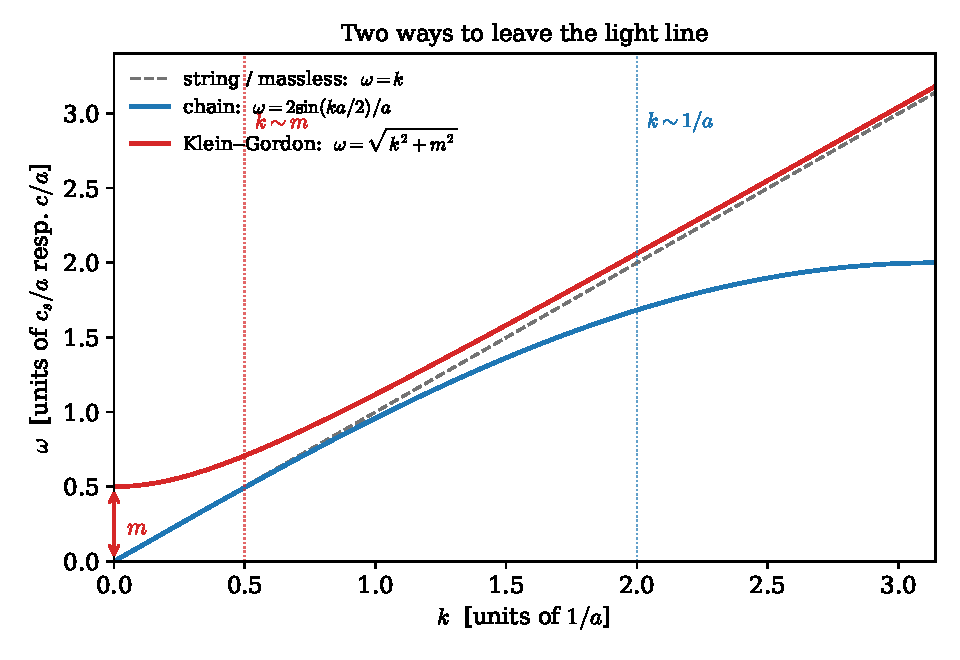
\includegraphics[width=0.8\textwidth]{fig_dispersion_trio.pdf}
  \caption{Three dispersion relations, drawn from their exact
  formulas ($c_s = c = 1$, lattice spacing $a = 1$, $m = 0.5$). The
  light line $\omega = k$ (gray, dashed) is left in two opposite
  directions: the chain [Osc.\ \S8.3] bends \emph{below} it at large
  $k$, where wavelengths approach the lattice spacing and the medium's
  discreteness shows; the Klein--Gordon field lifts \emph{above} it at
  small $k$, by the mass gap $\omega(0) = m$ --- every mattress
  element oscillates at $m$ even at infinite wavelength
  (Remark~\ref{rem:mattress}). Linear, light-like propagation
  survives only in the window $m \ll k \ll 1/a$: an ultraviolet scale
  and an infrared scale, bracketing the massless continuum from
  opposite sides.}
  \label{fig:dispersion-trio}
\end{figure}

\noindent
Figure~\ref{fig:dispersion-trio} assembles the Part's three
dispersion relations and reads as a summary of its physics: the
lattice scale $1/a$ bounds the wave regime from above (ultraviolet ---
the chain remembers its beads), the mass $m$ bounds it from below
(infrared --- the mattress remembers its tethers), and massless
light-line propagation is what both cutoffs leave between them. The
massive field is \emph{dispersive}: packets built from
\eqref{eq:KG-dispersion-eq} spread, because their Fourier components
travel at different group velocities --- in contrast to the massless
case, whose general solution $\phi = f(x - t) + g(x + t)$
[Osc.\ \S9.5] carries pulses
rigidly forever.

What the field equation cannot yet say is what the field
\emph{carries}: energy, momentum, and their currents. That is the
subject of Noether's theorem for fields --- the next section.

%=======================================================================
\section{Noether's Theorem for Fields}
%=======================================================================
\label{sec:noether-fields}

Noether's theorem for mechanics [Mech.\ \S3.3] traded each continuous
symmetry for a conserved \emph{number}. For fields the theorem returns
with a strictly stronger conclusion: each continuous symmetry yields a
conserved \emph{current} --- a local accounting of where the conserved
stuff sits and how it flows. This section proves the field version,
explains why relativity does not merely permit but \emph{demands} the
local form, and runs the theorem twice: on an internal symmetry (new
in kind --- nothing like it exists in Part I) and on spacetime
translations, whose four currents assemble into the energy-momentum
tensor.

\subsection{The theorem}
\label{sec:noether-theorem-fields}

\begin{definition}[Symmetry of a field theory]
A continuous transformation
$\phi \to \phi + \varepsilon\,\Delta\phi$ (with $\Delta\phi$ built
from $\phi$ and its derivatives) is a \emph{symmetry} if it changes
the Lagrangian density by at most a total divergence,
\begin{equation}
  \delta\mathcal L
  = \varepsilon\,\partial_\mu K^\mu
  \label{eq:quasi-symmetry}
\end{equation}
for some four-vector $K^\mu$ built from the fields --- for then
$\delta S$ is a pure boundary term and the equations of motion are
unchanged, exactly the logic of \S\ref{sec:gauge-coupling}. ($K^\mu = 0$
is the special case of exact invariance.)
\end{definition}

\begin{theorem}[Noether, field version]\label{thm:noether-fields}
If \eqref{eq:quasi-symmetry} holds, then along every solution of the
equations of motion \eqref{eq:covariant-EL} the current
\begin{equation}
  \boxed{\;
  j^\mu
  \;=\;
  \pd{\mathcal L}{(\partial_\mu\phi)}\,\Delta\phi
  \;-\; K^\mu
  \;}
  \label{eq:noether-current}
\end{equation}
is conserved:
\begin{equation}
  \boxed{\;\partial_\mu j^\mu = 0 .\;}
\end{equation}
(For several fields, sum the first term over them.)
\end{theorem}

\begin{proof}
Compute the change of $\mathcal L$ under the transformation by the
chain rule, in the slot-derivative sense of
\S\ref{sec:hamilton-fields}:
\begin{equation}
  \delta\mathcal L
  = \varepsilon\left[
    \pd{\mathcal L}{\phi}\,\Delta\phi
    + \pd{\mathcal L}{(\partial_\mu\phi)}\,
      \partial_\mu(\Delta\phi)
  \right].
\end{equation}
On a solution, the equation of motion \eqref{eq:covariant-EL} converts
the first coefficient:
$\partial\mathcal L/\partial\phi
= \partial_\mu\bigl(\partial\mathcal L/\partial(\partial_\mu\phi)\bigr)$.
The two terms then assemble into a total divergence by the product
rule:
\begin{equation}
  \delta\mathcal L
  = \varepsilon\,\partial_\mu\!\left[
    \pd{\mathcal L}{(\partial_\mu\phi)}\,\Delta\phi
  \right].
\end{equation}
Equating with the definition \eqref{eq:quasi-symmetry} of the
symmetry:
$\partial_\mu\bigl[
(\partial\mathcal L/\partial(\partial_\mu\phi))\Delta\phi - K^\mu
\bigr] = 0$, which is the claim.
\end{proof}

\subsection{What ``conserved'' now means: localization}
\label{sec:localization}

Unpack $\partial_\mu j^\mu = 0$ in $3{+}1$ language, writing
$j^\mu = (\rho, \vec\jmath\,)$:
\begin{equation}
  \boxed{\;
  \pd{\rho}{t} + \nabla\cdot\vec\jmath = 0
  \;}
  \qquad\text{--- a \emph{continuity equation}:}
  \label{eq:continuity}
\end{equation}
the density $\rho$ at a point can change only by flux $\vec\jmath$
through that point's neighborhood. Integrating over all space and
using the divergence theorem,
\begin{equation}
  \tot{Q}{t}
  = \tot{}{t}\int \rho\;\dd^3x
  = -\oint_{\partial} \vec\jmath \cdot \dd\vec A
  \;\longrightarrow\; 0
\end{equation}
for fields decaying at infinity (\S\ref{sec:boundary-terms}, fourth
mechanism): the global charge $Q = \int j^0\,\dd^3x$ is constant, and
mechanics' conclusion is recovered as a corollary. But the local
statement is the physics: the conserved stuff cannot vanish here and
reappear there --- it must \emph{flow through the intervening space},
and $\vec\jmath$ records the flow.

\begin{remark}[Why relativity demands the local form]
\label{rem:relativity-demands-local}
In Newtonian physics, local conservation is a refinement of global
conservation; in relativity it is the only coherent version. Suppose a
charge could teleport: vanish at event $P$ and appear at a distant
event $P'$, simultaneous with $P$ in some frame. $P$ and $P'$ are
spacelike separated, so their time order is frame-dependent
(\S\ref{sec:causal-structure}) --- boosted observers see the charge
appear \emph{before} it vanishes, or find slices of simultaneity
(\S\ref{sec:consequences}) on which total charge is doubled or absent.
``Total $Q$ at time $t$'' presupposes a simultaneity slicing, and
Part I spent a section showing that slicings are negotiable; the only
conservation statement all observers can share is the slicing-free,
pointwise \eqref{eq:continuity}. (Conversely, for a conserved current
the global $Q$ comes out the \emph{same} on every slicing --- $Q$ is
a Lorentz scalar. [stated; the proof integrates
$\partial_\mu j^\mu = 0$ over the region between two slices.])
\end{remark}

\subsection{First run: the complex scalar and its charge}
\label{sec:complex-scalar}

The theorem's first application is a symmetry of a kind Part I never
met. Package \emph{two} real Klein--Gordon fields of equal mass into
one complex field, $\phi = (\phi_1 + \ii\phi_2)/\sqrt2$, with density
\begin{equation}
  \mathcal L
  = \partial_\mu\phi^*\,\partial^\mu\phi
  - m^2\,\phi^*\phi
  \label{eq:complex-KG}
\end{equation}
(the $\tfrac12$'s of \eqref{eq:KG-lagrangian} absorbed by the
$\sqrt2$; and one standing trick, justified once: varying the
independent real fields $\phi_1, \phi_2$ is equivalent to varying
$\phi$ and $\phi^*$ \emph{as if independent} --- the two variation
bases are related by an invertible linear map, so stationarity in one
is stationarity in the other). Varying $\phi^*$ yields
$(\Box + m^2)\phi = 0$; varying $\phi$, the conjugate.

The point of the packaging: \eqref{eq:complex-KG} is exactly
invariant under the \emph{global phase rotation}
\begin{equation}
  \phi \to \ee^{-\ii\alpha}\phi,
  \qquad
  \phi^* \to \ee^{+\ii\alpha}\phi^*,
  \qquad \alpha \ \text{constant},
  \label{eq:U1}
\end{equation}
since every term pairs a $\phi$ with a $\phi^*$. This is an
\emph{internal} symmetry --- it turns the field's \emph{value},
touching the spacetime labels not at all --- the first symmetry of
the series with no spacetime meaning whatsoever, and the origin of
everything the word ``charge'' means in particle physics.
Infinitesimally, $\Delta\phi = -\ii\phi$,
$\Delta\phi^* = +\ii\phi^*$, with $K^\mu = 0$ (exact invariance), and
Theorem~\ref{thm:noether-fields} yields:
\begin{equation}
  j^\mu
  = \pd{\mathcal L}{(\partial_\mu\phi)}\,\Delta\phi
  + \pd{\mathcal L}{(\partial_\mu\phi^*)}\,\Delta\phi^*
  = (\partial^\mu\phi^*)(-\ii\phi)
  + (\partial^\mu\phi)(+\ii\phi^*),
\end{equation}
\begin{equation}
  \boxed{\;
  j^\mu = \ii\,\bigl(
    \phi^*\,\partial^\mu\phi
    - \phi\,\partial^\mu\phi^*
  \bigr),
  \qquad
  \partial_\mu j^\mu = 0 .
  \;}
  \label{eq:U1-current}
\end{equation}
The conservation deserves one direct check --- Noether proved it, but
the mechanism is instructive:
\begin{equation}
  \partial_\mu j^\mu
  = \ii\bigl(
      \phi^*\,\Box\phi - \phi\,\Box\phi^*
    \bigr)
  = \ii\bigl(
      \phi^*(-m^2\phi) - \phi(-m^2\phi^*)
    \bigr)
  = 0,
\end{equation}
the cross terms $\partial_\mu\phi^*\partial^\mu\phi$ canceling
identically and the mass terms canceling \emph{on shell}.

\begin{remark}[Charge, not probability]
\label{rem:charge-not-probability}
The charge density $j^0 = \ii(\phi^*\dot\phi - \phi\dot\phi^*)$ is
\textbf{not} positive definite --- complex conjugating a solution
flips its sign. Historically this killed the reading of $\phi$ as a
relativistic wavefunction with $j^0$ a probability density (the
Klein--Gordon equation's first, failed interpretation); rightly read, $Q$ is
a \emph{charge}, a quantity that legitimately comes in both signs ---
field and antifield, particle and antiparticle after quantization.
And the current will be needed again: \eqref{eq:U1-current} is
precisely the kind of object that can sit on the right-hand side of a
field equation for $A_\mu$ --- a conserved $J^\mu$ is what Part III's
Maxwell Lagrangian will demand as its source, and \emph{this} is
where such currents come from.
\end{remark}

\subsection{Second run: translations and the energy-momentum tensor}
\label{sec:T-mu-nu}

Now the central application: the four spacetime translations,
$x^\mu \to x^\mu + \varepsilon\,a^\mu$. A scalar field is dragged
along, $\phi(x) \to \phi(x - \varepsilon a)$, so
\begin{equation}
  \Delta\phi = -\,a^\nu\,\partial_\nu\phi .
\end{equation}
The density, having no explicit $x$-dependence, is dragged the same
way --- and \emph{that is already a total divergence}:
\begin{equation}
  \delta\mathcal L
  = -\,\varepsilon\, a^\nu\,\partial_\nu \mathcal L
  = \varepsilon\,\partial_\mu\bigl(-a^\mu\,\mathcal L\bigr),
  \qquad
  K^\mu = -\,a^\mu \mathcal L :
\end{equation}
a quasi-symmetry in the precise sense of \eqref{eq:quasi-symmetry},
with \emph{four} independent parameters $a^\nu$. Theorem
\ref{thm:noether-fields} gives the current
\begin{equation}
  j^\mu
  = \pd{\mathcal L}{(\partial_\mu\phi)}\,
    \bigl(-a^\nu\partial_\nu\phi\bigr)
    \;+\; a^\mu\,\mathcal L
  \;=\; -\,a^\nu \left[
    \pd{\mathcal L}{(\partial_\mu\phi)}\,\partial_\nu\phi
    - \delta^\mu{}_\nu\,\mathcal L
  \right],
\end{equation}
and since the four $a^\nu$ are independent, the bracket is conserved
for each $\nu$ separately --- four currents, organized as one
two-index object:
\begin{equation}
  \boxed{\;
  T^{\mu}{}_{\nu}
  \;=\;
  \pd{\mathcal L}{(\partial_\mu\phi)}\;\partial_\nu\phi
  \;-\; \delta^\mu{}_\nu\,\mathcal L,
  \qquad
  \partial_\mu T^{\mu}{}_{\nu} = 0
  \quad (\text{four equations, one per } \nu),
  \;}
  \label{eq:T-def}
\end{equation}
the \emph{energy-momentum tensor} (raising the second index,
$T^{\mu\nu} = (\partial\mathcal L/\partial(\partial_\mu\phi))
\partial^\nu\phi - \eta^{\mu\nu}\mathcal L$; it is a tensor by the
algebra of \S\ref{sec:tensors}, being built from tensors by products
and contractions). Its sixteen components record the field's entire
mechanics:
\begin{center}
\begin{tabular}{lll}
\toprule
component & name & role in \eqref{eq:continuity} \\
\midrule
$T^{00}$ & energy density & $\rho$ of the $\nu = 0$ current \\
$T^{i0}$ & energy flux & $\vec\jmath$ of the $\nu = 0$ current \\
$T^{0i}$ & momentum density & $\rho$ of the $\nu = i$ current \\
$T^{ji}$ & momentum flux (stress) & $\vec\jmath$ of the $\nu = i$ current \\
\bottomrule
\end{tabular}
\end{center}
and the four global charges are the field's four-momentum,
\begin{equation}
  P^\nu = \int T^{0\nu}\,\dd^3x
  = \bigl(E,\ \vec P\bigr),
\end{equation}
--- \S\ref{sec:particle-noether} rerun at field level, with the same
symmetry yielding the same conserved quantities, now \emph{localized}
into densities and fluxes.

\paragraph{The Klein--Gordon case.} For
\eqref{eq:KG-lagrangian}, $\partial\mathcal L/\partial(\partial_\mu\phi)
= \partial^\mu\phi$, so
$T^{\mu\nu} = \partial^\mu\phi\,\partial^\nu\phi - \eta^{\mu\nu}
\mathcal L$, and in particular
\begin{equation}
  \boxed{\;
  T^{00}
  = \tfrac12\,\dot\phi^2
  + \tfrac12\,|\nabla\phi|^2
  + \tfrac12\,m^2\phi^2
  \;\;\ge\; 0,
  \;}
  \qquad
  T^{0i} = \dot\phi\;\partial^i\phi .
  \label{eq:KG-T00}
\end{equation}
The energy density is a sum of three squares --- kinetic, gradient
(the tension energy of \S\ref{sec:wave-third-time}, one dimension up),
and tether (the mattress springs of Remark~\ref{rem:mattress}) ---
and its positivity is not accidental: it is the delayed consequence
of the sign choices of \S\ref{sec:building-lagrangians}. Flip the
kinetic sign and $T^{00}$ is unbounded below; flip the mass sign and
the tether term goes negative --- \S\ref{sec:building-lagrangians}'s
``signs are physics,'' made quantitative as a bounded energy. As a check against the series' oldest intuition: the same
formula \eqref{eq:T-def} applied to the string density gives energy
density $\tfrac12\mu\dot\phi^2 + \tfrac12 T\phi'^2$ and energy flux
$T^{x}{}_{0} = -T\phi'\dot\phi$ --- the transverse force
(\S\ref{sec:boundary-terms}) times the transverse velocity, i.e.\
mechanical power transmitted across the cross-section, exactly as a
free-body analysis would say.

\begin{remark}[The other six, and a symmetry requirement]
\label{rem:angular-momentum-fields}
The remaining Poincar\'e parameters (three rotations, three boosts;
Remark~\ref{rem:ten-charges}) yield, by the same theorem, the six
currents packaged as
$M^{\rho\mu\nu} = x^\mu\,T^{\rho\nu} - x^\nu\,T^{\rho\mu}$. Its
conservation is a one-line computation with a condition inside:
\begin{equation}
  \partial_\rho M^{\rho\mu\nu}
  = T^{\mu\nu} - T^{\nu\mu}
  + x^\mu\,\partial_\rho T^{\rho\nu}
  - x^\nu\,\partial_\rho T^{\rho\mu}
  = T^{\mu\nu} - T^{\nu\mu} :
\end{equation}
angular momentum is conserved \emph{if and only if the
energy-momentum tensor is symmetric}. For the scalar field it is,
automatically --- $\partial^\mu\phi\,\partial^\nu\phi$ and
$\eta^{\mu\nu}\mathcal L$ are symmetric by inspection. For fields
that carry indices of their own the canonical \eqref{eq:T-def} comes
out \emph{asymmetric}, the mismatch being the field's intrinsic
(spin) angular momentum, and a repair --- the Belinfante improvement,
adding a total-divergence term that symmetrizes $T$ without touching
the charges --- exists in general. [stated; Part III meets the
concrete case for the electromagnetic field in \S\ref{sec:gauge}, and
the general construction is QFT-course material.]
\end{remark}

\noindent
The Lagrangian story of the free scalar field is now complete:
equation of motion, symmetries, currents, energy. What remains of the
mechanics dictionary is its second column --- momenta, Hamiltonian,
brackets --- and porting it is the last stop before electromagnetism.

%=======================================================================
\section{Hamiltonian Field Theory}
%=======================================================================
\label{sec:hamiltonian-fields}

One column of the mechanics dictionary remains untranslated: momenta,
Hamiltonian, brackets --- the phase-space half of [Mech.\ Part II].
This section ports it, with one genuinely new ingredient (the Dirac
delta, introduced as what it is rather than what it is written as)
and one promise kept: Remark~\ref{rem:H-not-covariant}
stated that the particle's trade --- manifest covariance given up
at the Legendre transform --- would recur, unchanged, for fields.

\subsection{The field momentum and the Hamiltonian}
\label{sec:field-momentum}

The dictionary of \S\ref{sec:pivot} translates
$p_i = \partial L/\partial\dot q_i$ entry by entry: one momentum per
degree of freedom, i.e.\ one per point,
\begin{equation}
  \boxed{\;
  \pi(\vx)
  \;\equiv\;
  \frac{\delta L}{\delta\dot\phi(\vx)}
  \;=\;
  \pd{\mathcal L}{\dot\phi}
  \;}
  \label{eq:field-momentum}
\end{equation}
(the two expressions agree because $\mathcal L$ contains no spatial
derivatives of $\dot\phi$ --- nothing for
\eqref{eq:functional-derivative}'s integration by parts to move). For
Klein--Gordon, $\pi = \dot\phi$; for the complex scalar
\eqref{eq:complex-KG}, note the crossing, $\pi = \dot\phi^*$ and
$\pi^* = \dot\phi$. The Legendre transform [Mech.\ \S6.1] then runs
pointwise --- one transform per degree of freedom, aggregated by the
dictionary's $\int\dd^3x$:
\begin{equation}
  \boxed{\;
  H = \int \dd^3x\;\mathcal H,
  \qquad
  \mathcal H
  = \pi\,\dot\phi - \mathcal L
  \quad (\dot\phi \text{ eliminated in favor of } \pi).
  \;}
\end{equation}
For Klein--Gordon, $\dot\phi = \pi$ inverts trivially and
\begin{equation}
  \mathcal H
  = \tfrac12\,\pi^2
  + \tfrac12\,|\nabla\phi|^2
  + \tfrac12\, m^2\phi^2
  \;=\; T^{00}\big|_{\dot\phi\to\pi} :
  \label{eq:KG-hamiltonian-density}
\end{equation}
the Hamiltonian density \emph{is} the energy density
\eqref{eq:KG-T00} --- the field-theory instance of [Mech.\ \S6.3]'s
``$H = T + V$ for a kinetic term purely quadratic in the velocities
and a velocity-independent potential,''
and positive definite for the reasons established in \S\ref{sec:T-mu-nu}.

\emph{The discrete check, third installment.} On the chain,
$p_j = m\dot y_j = (\mu a)\,\dot\phi(x_j) = a\,\pi(x_j)$: the bead's
momentum is the momentum \emph{density} times the cell size --- the
same factor of $a$ as in \S\ref{sec:functional-derivative}, now on the
conjugate variable. The two cell factors then combine correctly in
the Hamiltonian:
$\sum_j p_j^2/(2m) = \sum_j a\,\pi(x_j)^2/(2\mu)
\to \int\dd x\, \pi^2/(2\mu)$, the kinetic term of
\eqref{eq:KG-hamiltonian-density} (with the string's $\mu$, absorbed
to $1$ in the Klein--Gordon normalization).

\subsection{The Dirac delta as a distribution}
\label{sec:dirac-delta}

Phase-space mechanics needs one more derivative the Lagrangian story
never asked for: the sensitivity of a \emph{local} quantity to a
local change --- $\delta\phi(\vec y)/\delta\phi(\vx)$, the field-theory
descendant of $\partial q_i/\partial q_j = \delta_{ij}$. Apply the
definition \eqref{eq:functional-derivative} to the evaluation
functional $F[\phi] = \phi(\vec y)$: its variation under
$\phi \to \phi + \varepsilon\eta$ is exactly $\varepsilon\,\eta(\vec y)$,
so the sought object is whatever satisfies
\begin{equation}
  \int \dd^3x\;
  \frac{\delta\phi(\vec y)}{\delta\phi(\vx)}\;
  \eta(\vx)
  = \eta(\vec y)
  \qquad\text{for every test function } \eta .
  \label{eq:delta-defining}
\end{equation}
No function does this --- a function vanishing away from one point
integrates to zero against everything --- but
\eqref{eq:delta-defining} itself is a perfectly good definition of a
different kind of object: a \emph{distribution}, a linear machine
that takes a test function and returns a number, written
\emph{as if} it were an integral kernel:
\begin{equation}
  \boxed{\;
  \frac{\delta\phi(\vec y)}{\delta\phi(\vx)}
  = \delta^3(\vx - \vec y),
  \qquad
  \int\dd^3 x\;\delta^3(\vx - \vec y)\,f(\vx) = f(\vec y).
  \;}
  \label{eq:delta}
\end{equation}
The integral notation is a fiction with a license: every manipulation
performed on $\delta$ in this document (integration against smooth
functions, integration by parts, change of variables) is the shadow
of a legitimate operation on the underlying functional, and
Appendix~\ref{app:distributions} sets out the small amount of theory
that issues the license. The dictionary, meanwhile, closes its last
entry with the same cell factor as always:
\begin{equation}
  \pd{y_i}{y_j} = \delta_{ij}
  \qquad\longleftrightarrow\qquad
  \frac{\delta\phi(x_i)}{\delta\phi(x_j)}
  = \frac{\delta_{ij}}{a}\;\to\;\delta(x_i - x_j) :
\end{equation}
the Kronecker delta \emph{per cell volume} is the discrete Dirac
delta --- check: $\sum_j a\,(\delta_{ij}/a)\,f_j = f_i$ mirrors
\eqref{eq:delta} term for term --- and it correctly blows up as
$a \to 0$: sensitivity \emph{density} to a single point must be
infinite if its integral over a shrinking cell is to stay one.

\subsection{Poisson brackets and Hamilton's equations}
\label{sec:field-poisson}

Port the bracket of [Mech.\ \S8.1] through the dictionary --- sum to
integral, partials to functional derivatives:
\begin{equation}
  \{F, G\}
  \;=\;
  \int \dd^3x
  \left[
    \frac{\delta F}{\delta\phi(\vx)}\,
    \frac{\delta G}{\delta\pi(\vx)}
    -
    \frac{\delta F}{\delta\pi(\vx)}\,
    \frac{\delta G}{\delta\phi(\vx)}
  \right],
  \label{eq:field-bracket}
\end{equation}
inheriting antisymmetry, bilinearity, Leibniz, and Jacobi from the
mechanical original (the proofs [Mech.\ \S8.1, App.\ F] transcribe
line by line). The fundamental brackets follow from
\eqref{eq:delta}: with $F = \phi(\vx)$, $G = \pi(\vec y)$,
\begin{equation}
  \{\phi(\vx),\, \pi(\vec y)\}
  = \int\dd^3z\;
    \delta^3(\vec z - \vx)\,\delta^3(\vec z - \vec y)
  = \delta^3(\vx - \vec y),
\end{equation}
\begin{equation}
  \boxed{\;
  \{\phi(\vx), \pi(\vec y)\} = \delta^3(\vx - \vec y),
  \qquad
  \{\phi, \phi\} = \{\pi, \pi\} = 0
  \qquad(\text{equal times}).
  \;}
  \label{eq:fundamental-brackets}
\end{equation}
Dynamics is bracket flow, as in [Mech.\ \S8.2]:
$\dot F = \{F, H\}$, and in particular
\begin{equation}
  \dot\phi = \frac{\delta H}{\delta\pi} ,
  \qquad
  \dot\pi = -\,\frac{\delta H}{\delta\phi} .
  \label{eq:field-hamilton-eqs}
\end{equation}
\emph{The Klein--Gordon check.} From
\eqref{eq:KG-hamiltonian-density}: $\delta H/\delta\pi = \pi$, so
$\dot\phi = \pi$, recovering the definition; and --- here the
integration by parts built into \eqref{eq:functional-derivative}
acts on the gradient term ---
\begin{equation}
  \dot\pi
  = -\frac{\delta H}{\delta\phi}
  = \nabla\cdot(\nabla\phi) - m^2\phi
  = \nabla^2\phi - m^2\phi .
\end{equation}
Combining, $\ddot\phi = \nabla^2\phi - m^2\phi$ --- the Klein--Gordon
equation \eqref{eq:KG}, re-derived from the phase-space side. And one
sentence that the outlook will inflate: promoting the classical
bracket \eqref{eq:fundamental-brackets} to a commutator,
$[\hat\phi(\vx), \hat\pi(\vec y)] = \ii\,\delta^3(\vx - \vec y)$, is
the \emph{first move} of canonical quantization --- the entire
apparatus of this section is its starting point.

\begin{remark}[The slicing trade returns for fields]
\label{rem:slicing-again}
Remark~\ref{rem:H-not-covariant} described this trade for the
particle; here it recurs for fields, in identical form --- which is
the point.
The momentum \eqref{eq:field-momentum} differentiates with respect to
\emph{somebody's} $\dot\phi$; the brackets
\eqref{eq:fundamental-brackets} are \emph{equal-time} brackets,
defined on a slice; and the Hamiltonian is
$H = \int T^{00}\,\dd^3x = P^0$ --- the $00$-component of a tensor,
integrated over the chosen slice, the time component of the field's
four-momentum. Different observers slice differently and carry
different Hamiltonians. Covariance survives as a theorem with the
same statement as before: the ten Poincar\'e charges --- $P^\mu$ from
\S\ref{sec:T-mu-nu}, $M^{\mu\nu}$ from
Remark~\ref{rem:angular-momentum-fields} --- close under the bracket
\eqref{eq:field-bracket} into the Poincar\'e algebra, boost charges
explicitly time-dependent, conservation by the same cancellation as
in Remark~\ref{rem:H-not-covariant}. [stated; verifying the algebra is a
long computation, not run here.] Canonical quantization inherits
every word of this, and ``the quantum field theory is Lorentz
invariant'' is a statement about operator charges, proved, not seen
--- while the path integral, built on the scalar $S[\phi]$ of
\S\ref{sec:covariant-EL}, keeps covariance manifest throughout. The
two quantization routes part company exactly here, at a fork Part I's
free particle already mapped.
\end{remark}

%=======================================================================
\clearpage
\part{The Electromagnetic Field}
%=======================================================================

%=======================================================================
\section{The Field Tensor}
%=======================================================================
\label{sec:field-tensor}

Part I left electromagnetism half-told: the potentials $A^\mu$
entered as a background, the variational principle manufactured the
antisymmetric combination $F_{\mu\nu}$
(Eq.~\eqref{eq:covariant-lorentz-force}), and the quotient rule
certified it as a tensor. This section opens Part III by taking the
tensor seriously as an object: its components are $\vE$ and $\vB$,
its transformation law is the long-sought answer to ``how do
electric and magnetic fields look from a moving frame,'' and its two
invariants are the only field statements all observers share. The
section closes by building the object that will source the dynamics:
the four-current.

\subsection{The six components}
\label{sec:six-components}

From \S\ref{sec:lorentz-force}, with $A^\mu = (\varphi, \vec A)$,
$A_\mu = (\varphi, -\vec A)$:
\begin{equation}
  F_{\mu\nu} = \partial_\mu A_\nu - \partial_\nu A_\mu,
  \qquad
  \vE = -\nabla\varphi - \partial_t\vec A,
  \qquad
  \vB = \nabla\times\vec A .
\end{equation}
Antisymmetry kills the diagonal and pairs the rest: $6$ independent
components, and \S\ref{sec:lorentz-force} claimed they are exactly the
six numbers above. Verify by direct evaluation. Time-space:
\begin{equation}
  F_{0i}
  = \partial_0 A_i - \partial_i A_0
  = \partial_t(-A^i) - \partial_i\varphi
  = \Bigl(-\nabla\varphi - \partial_t\vec A\Bigr)_{\!i}
  = E_i .
\end{equation}
Space-space:
\begin{equation}
  F_{ij}
  = \partial_i A_j - \partial_j A_i
  = -\bigl(\partial_i A^j - \partial_j A^i\bigr)
  = -\,\epsilon_{ijk}\,B_k ,
\end{equation}
(the middle sign from lowering two spatial indices; the last equality
is the component form of the curl). Assembled, with rows $\mu$ and
columns $\nu$:
\begin{equation}
  F_{\mu\nu} =
  \begin{pmatrix}
    0 & E_x & E_y & E_z \\
    -E_x & 0 & -B_z & B_y \\
    -E_y & B_z & 0 & -B_x \\
    -E_z & -B_y & B_x & 0
  \end{pmatrix},
  \qquad
  F^{\mu\nu} =
  \begin{pmatrix}
    0 & -E_x & -E_y & -E_z \\
    E_x & 0 & -B_z & B_y \\
    E_y & B_z & 0 & -B_x \\
    E_z & -B_y & B_x & 0
  \end{pmatrix}
  \label{eq:F-matrix}
\end{equation}
(raising both indices flips only the mixed time-space entries:
$F^{0i} = \eta^{00}\eta^{ij}F_{0j} = -F_{0i}$, while
$F^{ij} = F_{ij}$). The moral outranks the matrix: \emph{$\vE$ and
$\vB$ are not two vector fields}. They are the time-space and
space-space slices of one antisymmetric tensor --- a split made by a
choice of frame, with no invariant meaning --- and every ``mystery''
of their mixing is the ordinary behavior of tensor components under
Eq.~\eqref{eq:tensor-law}.

\subsection{How $\vE$ and $\vB$ transform}
\label{sec:E-B-transform}

The tensor law now delivers what \S\ref{sec:tensors} promised: the
transformation of $\vE$ and $\vB$ for free. Boost along $x$ with
velocity $\beta$ and apply
$F'^{\mu\nu} = \Lambda^\mu{}_\rho \Lambda^\nu{}_\sigma F^{\rho\sigma}$.
Two representative components, in full. The $(01)$ entry meets both
boost rows:
\begin{equation}
  F'^{01}
  = \Lambda^0{}_0\Lambda^1{}_1\,F^{01}
  + \Lambda^0{}_1\Lambda^1{}_0\,F^{10}
  = \gamma^2 F^{01} + \gamma^2\beta^2 F^{10}
  = \gamma^2(1 - \beta^2)\,F^{01}
  = F^{01} ,
\end{equation}
so $E'_x = E_x$: the component along the boost is untouched (the two
$\gamma$'s and the antisymmetry combine to cancel). The $(02)$ entry
meets one boost row and one spectator:
\begin{equation}
  F'^{02}
  = \Lambda^0{}_0\,F^{02} + \Lambda^0{}_1\,F^{12}
  = \gamma\,(-E_y) + (-\gamma\beta)(-B_z)
  \;\Longrightarrow\;
  E'_y = \gamma\bigl(E_y - \beta B_z\bigr) .
\end{equation}
The remaining components run identically, and the complete result is:
\begin{center}
\begin{tabular}{ll}
\toprule
parallel to the boost & transverse to the boost \\
\midrule
$E'_x = E_x$ &
$E'_y = \gamma\,(E_y - \beta B_z)$
\hspace{1.2em}
$E'_z = \gamma\,(E_z + \beta B_y)$ \\[3pt]
$B'_x = B_x$ &
$B'_y = \gamma\,(B_y + \beta E_z)$
\hspace{1.05em}
$B'_z = \gamma\,(B_z - \beta E_y)$ \\
\bottomrule
\end{tabular}
\end{center}
Compactly: $\vE_\parallel$, $\vB_\parallel$ inert;
$\vE'_\perp = \gamma(\vE + \vec\beta\times\vB)_\perp$,
$\vB'_\perp = \gamma(\vB - \vec\beta\times\vE)_\perp$. Electric and
magnetic fields feed each other under boosts, in exactly the way
$t$ and $x$ do.

\begin{remark}[Magnetism is boosted electricity]
\label{rem:magnetism-is-relativity}
The table contains a physical point usually buried in a third
course on the subject. Take a single charge at rest: pure Coulomb
$\vE$, no $\vB$ anywhere (elementary electrostatics, imported here as
input; \S\ref{sec:maxwell-lagrangian} derives the field equations, and
Example~\ref{ex:coulomb} the field). View it from a moving frame: the table
manufactures $\vB'_\perp = -\gamma(\vec\beta\times\vE)_\perp \neq 0$
--- a magnetic field, from nothing but a boost. Magnetism is not a
second force; it is what electrostatics looks like from a frame in
which the charges move, and its everyday effects are large not
because $\beta$ is large (drift velocities in wires are
$\mathrm{mm/s}$, $\beta \sim 10^{-12}$) but because the electrostatic
force it corrects is enormous --- wires are neutral to
extraordinary precision, and the magnetic force between them is the
$O(\beta^2)$ relativistic residue of two large, nearly perfectly
canceling electric forces. [The quantitative wire analysis --- length
contraction unbalancing the two charge densities --- is a classic
worked example; stated here, not run.] Historically the logic ran
backwards: Einstein's 1905 paper is titled ``On the Electrodynamics
of Moving Bodies,'' and its opening paragraph is precisely the
magnet-and-conductor asymmetry this remark dissolves.
\end{remark}

\subsection{The two invariants}
\label{sec:two-invariants}

What do all observers agree on? Full contractions
(\S\ref{sec:tensors}). With one tensor and the metric, exactly one is
available:
\begin{equation}
  F_{\mu\nu}F^{\mu\nu}
  = 2\,F_{0i}F^{0i} + F_{ij}F^{ij}
  = -2\,\vE^2
  + \epsilon_{ijk}\epsilon_{ijl}B_k B_l
  \;\Longrightarrow\;
  \boxed{\;
  F_{\mu\nu}F^{\mu\nu} = 2\bigl(\vB^2 - \vE^2\bigr),
  \;}
  \label{eq:invariant-1}
\end{equation}
using $\epsilon_{ijk}\epsilon_{ijl} = 2\delta_{kl}$. A second
invariant needs the last invariant tensor, now introduced as
\S\ref{sec:tensors} promised: the totally antisymmetric
$\epsilon^{\mu\nu\rho\sigma}$, fixed by
$\epsilon^{0123} = +1$. It is invariant under the proper
orthochronous transformations only ---
$\Lambda^\mu{}_\alpha\Lambda^\nu{}_\beta\Lambda^\rho{}_\gamma
\Lambda^\sigma{}_\delta\,\epsilon^{\alpha\beta\gamma\delta}
= (\det\Lambda)\,\epsilon^{\mu\nu\rho\sigma}$, the definition of the
determinant --- so objects built with one $\epsilon$ flip sign under
$P$ or $T$ (\emph{pseudo}-scalars and pseudo-tensors). Define the
\emph{dual} tensor and evaluate its slices by the same component
patience as \eqref{eq:F-matrix}:
\begin{equation}
  \tilde F^{\mu\nu}
  \equiv \tfrac12\,\epsilon^{\mu\nu\rho\sigma}F_{\rho\sigma},
  \qquad
  \tilde F^{0i} = -B_i,
  \quad
  \tilde F^{ij} = \epsilon_{ijk}\,E_k
  \qquad
  \text{--- i.e.\ } (\vE, \vB) \to (\vB,\, -\vE) :
\end{equation}
duality trades the two fields. The second invariant:
\begin{equation}
  F_{\mu\nu}\tilde F^{\mu\nu}
  = 2F_{0i}\tilde F^{0i} + F_{ij}\tilde F^{ij}
  = -2\,\vE\cdot\vB - 2\,\vE\cdot\vB
  \;\Longrightarrow\;
  \boxed{\;
  F_{\mu\nu}\tilde F^{\mu\nu} = -\,4\,\vE\cdot\vB
  \;}
  \label{eq:invariant-2}
\end{equation}
(a pseudo-scalar: it flips under $P$, as $\vE\cdot\vB$ visibly does,
$\vE$ being a vector and $\vB$ an axial vector). These two numbers
are the entire frame-independent content of a field configuration at
a point, and they sort configurations into invariant classes:
if $\vE \perp \vB$ in one frame, then in all; if $\vE \cdot \vB \neq 0$,
both fields are nonzero in \emph{every} frame, and no purely electric
or purely magnetic frame exists; if $\vE \cdot \vB = 0$ and
$\vB^2 > \vE^2$, some frame sees a pure magnetic field (and
symmetrically for $\vE^2 > \vB^2$); and the doubly-null case
\begin{equation}
  \vE^2 = \vB^2,
  \qquad
  \vE \cdot \vB = 0
  \qquad(\text{both invariants zero})
\end{equation}
is a class of its own --- \emph{null fields}, perpendicular and
equal-magnitude in \emph{every} frame, with no rest frame to boost
to. Section~\ref{sec:gauge} will find exactly this signature in the
electromagnetic wave: light is null, in every sense this document has
given the word.

\subsection{The four-current}
\label{sec:four-current}

Dynamics needs a source, and \S\ref{sec:complex-scalar} specified
what one must be: a conserved four-vector current. Electromagnetism's
version packages charge density and current density,
\begin{equation}
  J^\mu = \bigl(\rho,\ \vec J\bigr),
\end{equation}
and its four-vector credentials rest on one experimental scalar:
\emph{electric charge is Lorentz invariant} (an electron's charge
does not depend on its speed --- verified to extraordinary precision
by the neutrality of atoms, whose electrons move and whose protons'
quarks move very differently [experimental input]). For a flow of
charges of proper density $\rho_0$ (density in the local rest frame,
a scalar) moving with four-velocity $u^\mu(x)$:
\begin{equation}
  J^\mu = \rho_0\, u^\mu
  = \bigl(\gamma\rho_0,\ \gamma\rho_0\vec v\,\bigr)
  \label{eq:convective-current}
\end{equation}
--- scalar times four-vector, credentials immediate; the $\gamma$ in
$\rho = \gamma\rho_0$ is length contraction acting on the volume in
the denominator of ``charge per volume,'' charge itself inert. A
general $J^\mu$ is a superposition of such flows. Conservation of
charge is then the continuity equation of \S\ref{sec:localization},
\begin{equation}
  \boxed{\;
  \partial_\mu J^\mu = 0
  \qquad\Longleftrightarrow\qquad
  \pd{\rho}{t} + \nabla\cdot\vec J = 0,
  \;}
  \label{eq:charge-continuity}
\end{equation}
with Remark~\ref{rem:relativity-demands-local} supplying the reason
this \emph{must} be the local statement. For now
\eqref{eq:charge-continuity} is an empirical fact about the source;
\S\ref{sec:maxwell-lagrangian} will show the field equations
\emph{enforce} it --- a source that fails to conserve charge cannot
couple to the electromagnetic field at all --- and
\S\ref{sec:complex-scalar}'s Noether current is the standing example
of where a microscopic theory gets such a $J^\mu$ from.

%=======================================================================
\section{The Maxwell Lagrangian}
%=======================================================================
\label{sec:maxwell-lagrangian}

Now the building-block game of \S\ref{sec:building-lagrangians},
replayed for the vector field --- with one extra constraint. For the
scalar, the covariance principle alone thinned the catalogue; for
$A_\mu$, the redundancy met in \S\ref{sec:gauge-coupling} also
constrains: \emph{the action may change by at most boundary terms under}
$A_\mu \to A_\mu + \partial_\mu\chi$, or the unphysical redundancy would
leak into the dynamics. The two constraints turn out to leave essentially
one theory standing, and its equations of motion are Maxwell's.

\subsection{Building the Lagrangian under two constraints}
\label{sec:building-maxwell}

Candidates quadratic in $A_\mu$ (free-field logic, as in
\S\ref{sec:building-lagrangians}), screened in order:
\begin{itemize}
  \item \textbf{The mass term $A_\mu A^\mu$.} A perfectly good Lorentz
  scalar --- but not gauge invariant: it shifts by
  $2A^\mu\partial_\mu\chi + \partial_\mu\chi\,\partial^\mu\chi$, no
  total divergence for generic $\chi$. A photon mass is not merely
  inelegant; it is \emph{incompatible with the redundancy}, which is
  why its experimental bound is a test of the framework
  ($m_\gamma < 10^{-18}\,\mathrm{eV}$ [experimental input]).
  \item \textbf{Generic derivative quadratics}
  ($\partial_\mu A_\nu\,\partial^\mu A^\nu$,
  $(\partial_\mu A^\mu)^2$, \dots). Individually gauge-variant. The
  \emph{only} first-derivative combination inert under the gauge
  shift is the one the particle's variational principle manufactured
  in \S\ref{sec:lorentz-force}: $F_{\mu\nu}$, gauge-invariant because
  $\partial_\mu\partial_\nu\chi$ is symmetric
  (Proposition~\ref{prop:sym-antisym} in action). Scalars built from
  it: $F_{\mu\nu}F^{\mu\nu}$ and $F_{\mu\nu}\tilde F^{\mu\nu}$.
  \item \textbf{The dual candidate $F\tilde F$} drops out:
  it is a total divergence,
  \begin{equation}
    F_{\mu\nu}\tilde F^{\mu\nu}
    = 2\,\epsilon^{\mu\nu\rho\sigma}\,
      \partial_\mu A_\nu\,\partial_\rho A_\sigma
    = 2\,\partial_\mu\!\bigl(
        \epsilon^{\mu\nu\rho\sigma} A_\nu\,\partial_\rho A_\sigma
      \bigr),
  \end{equation}
  the second equality because pulling $\partial_\mu$ out costs a term
  $\epsilon^{\mu\nu\rho\sigma}A_\nu\partial_\mu\partial_\rho A_\sigma$
  that dies on Proposition~\ref{prop:sym-antisym}
  ($\partial_\mu\partial_\rho$ symmetric, $\epsilon$ antisymmetric).
  Boundary terms do not affect the equations of motion, so
  $F\tilde F$ contributes nothing classically.
  (Its quantum role --- topological terms, anomalies --- is real
  and deferred. [stated.])
\end{itemize}
One field-only candidate survives. Fix its normalization by
expanding in $3{+}1$ language via \eqref{eq:invariant-1}:
\begin{equation}
  -\tfrac14\, F_{\mu\nu}F^{\mu\nu}
  = \tfrac12\bigl(\vE^2 - \vB^2\bigr),
\end{equation}
and since $\vE$ carries the time derivatives of the potentials
(Eq.~\eqref{eq:E-B-definitions}), the coefficient $-\tfrac14$ is
exactly what gives the kinetic terms the scalar field's $+\tfrac12$
normalization --- kinetic minus potential, matching
\eqref{eq:KG-31}.

The source coupling is the linear term $-J^\mu A_\mu$, with $J^\mu$
a prescribed external current --- and here the gauge constraint
becomes decisive. Under the gauge shift,
\begin{equation}
  -\,J^\mu\,\partial_\mu\chi
  = -\,\partial_\mu\bigl(J^\mu \chi\bigr)
  \;+\; \chi\,\partial_\mu J^\mu :
  \label{eq:gauge-forces-conservation}
\end{equation}
a total divergence \emph{if and only if} $\partial_\mu J^\mu = 0$.
Gauge invariance does not merely tolerate the conservation law of
\S\ref{sec:four-current} --- it \emph{demands} it, before a single
equation of motion has been derived: a non-conserved current cannot
be coupled to the electromagnetic field at all. Assembling:
\begin{equation}
  \boxed{\;
  \mathcal L
  \;=\;
  -\,\tfrac14\, F_{\mu\nu}F^{\mu\nu}
  \;-\; J^\mu A_\mu .
  \;}
  \label{eq:maxwell-lagrangian}
\end{equation}

\begin{remark}[Units in Part III]\label{rem:units-EM}
The normalization of \eqref{eq:maxwell-lagrangian} fixes the
electromagnetic unit system: these are rationalized
Heaviside--Lorentz units (with $c = 1$ as always), in which no factors
of $4\pi$ appear in the field equations. Restoring SI expressions ---
as Example~\ref{ex:sunlight} will do --- reinstates $\varepsilon_0$
and $\mu_0$ by dimensional analysis, in the same way
Convention~\ref{conv:units} restores $c$. [stated; the conversion
between unit systems is standard.]
\end{remark}

\subsection{Variation: the inhomogeneous pair}
\label{sec:inhomogeneous}

The field Euler--Lagrange equation \eqref{eq:covariant-EL} runs once
per component of $A_\nu$ --- four fields, one shared index. The
derivative of the kinetic term is the section's one full index
computation, so it is displayed whole. Write
$F_{\rho\sigma}F^{\rho\sigma}
= 2\bigl(\partial_\rho A_\sigma\,\partial^\rho A^\sigma
- \partial_\rho A_\sigma\,\partial^\sigma A^\rho\bigr)$; then, with
the renaming discipline of Rule 6 (\S\ref{sec:index-grammar}),
\begin{equation}
  \pd{}{(\partial_\mu A_\nu)}
  \bigl(\partial_\rho A_\sigma\,\partial^\rho A^\sigma\bigr)
  = 2\,\partial^\mu A^\nu,
  \qquad
  \pd{}{(\partial_\mu A_\nu)}
  \bigl(\partial_\rho A_\sigma\,\partial^\sigma A^\rho\bigr)
  = 2\,\partial^\nu A^\mu,
\end{equation}
(each factor contributes once, the metric raising what the Kronecker
deltas deliver), so
\begin{equation}
  \pd{\mathcal L}{(\partial_\mu A_\nu)}
  = -\tfrac14 \cdot 2\,
    \bigl(2\,\partial^\mu A^\nu - 2\,\partial^\nu A^\mu\bigr)
  = -\,F^{\mu\nu},
  \qquad
  \pd{\mathcal L}{A_\nu} = -\,J^\nu ,
\end{equation}
and \eqref{eq:covariant-EL} reads
$\partial_\mu(-F^{\mu\nu}) = -J^\nu$:
\begin{equation}
  \boxed{\;
  \partial_\mu F^{\mu\nu} = J^\nu .
  \;}
  \label{eq:maxwell-inhomogeneous}
\end{equation}
Unpack with the matrix \eqref{eq:F-matrix} ($F^{i0} = E_i$,
$F^{ij} = -\epsilon_{ijk}B_k$). The $\nu = 0$ component:
\begin{equation}
  \partial_i F^{i0} = J^0
  \qquad\Longrightarrow\qquad
  \nabla\cdot\vE = \rho
  \qquad\text{(Gauss)},
\end{equation}
and $\nu = j$:
\begin{equation}
  \partial_0 F^{0j} + \partial_i F^{ij} = J^j
  \qquad\Longrightarrow\qquad
  \nabla\times\vB - \pd{\vE}{t} = \vec J
  \qquad\text{(Amp\`ere--Maxwell)},
\end{equation}
using $\partial_i F^{ij} = -\epsilon_{ijk}\partial_i B_k
= (\nabla\times\vB)_j$. Two of Maxwell's four equations, from one
variation.

\paragraph{The field equations enforce charge conservation.} Act with $\partial_\nu$
on \eqref{eq:maxwell-inhomogeneous}:
\begin{equation}
  \partial_\nu J^\nu
  = \partial_\nu \partial_\mu F^{\mu\nu}
  = 0
  \qquad\text{identically}
\end{equation}
--- Proposition~\ref{prop:sym-antisym} once more, symmetric
$\partial_\nu\partial_\mu$ against antisymmetric $F^{\mu\nu}$. The
requirement of \S\ref{sec:four-current} is now enforced from both ends:
gauge invariance demanded a conserved source before the dynamics
existed (\ref{eq:gauge-forces-conservation}), and the dynamics, once
derived, is structurally incapable of sourcing itself from anything
else. That one three-line proposition from the grammar section
is behind gauge invariance of $F$, the inertness of $F\tilde F$,
and charge conservation --- three results, one identity.

\begin{example}[The static point charge]\label{ex:coulomb}
The simplest solution of \eqref{eq:maxwell-inhomogeneous}. Put a single
charge $q$ at rest at the origin: $\rho = q\,\delta^3(\vx)$,
$\vec J = 0$ --- the delta of \S\ref{sec:dirac-delta} placing the whole
charge at one point (\S\ref{sec:one-coupling} exhibits this as the
static case of a worldline current). Seek a static, spherically
symmetric field --- the source distinguishes no direction and no time
--- so try $\vE = E(r)\,\hat r$ with $\vB = 0$. Integrate Gauss's law
over a ball of radius $r$ and apply the divergence theorem, as in
\S\ref{sec:localization}:
\begin{equation}
  \oint_{S_r} \vE\cdot\dd\vec A
  = 4\pi r^2\,E(r)
  = \int_{B_r} q\,\delta^3(\vx)\;\dd^3x
  = q ,
\end{equation}
so
\begin{equation}
  \boxed{\;
  \vE = \frac{q}{4\pi r^2}\,\hat r
  \;}
  \qquad
  \Bigl(\text{equivalently } \varphi = \frac{q}{4\pi r},\ \vec A = 0:
  \text{ check } -\nabla\varphi = \vE,\ \vB = \nabla\times\vec A = 0\Bigr).
\end{equation}
The $4\pi$ of Heaviside--Lorentz units (Remark~\ref{rem:units-EM}) sits
in the field, not in the field equation. This is the pure-electric
configuration that Remark~\ref{rem:magnetism-is-relativity} boosted;
that it is the \emph{only} static solution decaying at infinity is a
uniqueness statement not proved here. [stated.]
\end{example}

\subsection{The homogeneous pair: geometry, not dynamics}
\label{sec:bianchi}

Two Maxwell equations remain, and no variation will produce them ---
because they are not dynamics. They are \emph{identities}, true of
any $F$ built from a potential. Substitute
$F_{\mu\nu} = \partial_\mu A_\nu - \partial_\nu A_\mu$ into the
cyclic sum:
\begin{align}
  \partial_\mu F_{\nu\rho}
  + \partial_\nu F_{\rho\mu}
  + \partial_\rho F_{\mu\nu}
  &= \bigl(\partial_\mu\partial_\nu A_\rho
         - \partial_\mu\partial_\rho A_\nu\bigr)
   + \bigl(\partial_\nu\partial_\rho A_\mu
         - \partial_\nu\partial_\mu A_\rho\bigr)
   + \bigl(\partial_\rho\partial_\mu A_\nu
         - \partial_\rho\partial_\nu A_\mu\bigr)
  \notag\\
  &= 0,
\end{align}
the six terms canceling in pairs (first with fourth, second with
fifth, third with sixth --- equality of mixed partials each time).
This is the \emph{Bianchi identity}; contracting it with
$\tfrac12\epsilon^{\lambda\mu\nu\rho}$ packages the same statement as
\begin{equation}
  \boxed{\;
  \partial_\mu \tilde F^{\mu\nu} = 0 ,
  \;}
  \label{eq:maxwell-homogeneous}
\end{equation}
($\epsilon$ picks out exactly the totally antisymmetric part of
$\partial F$, which is what the cyclic sum is). Unpack with
$\tilde F^{i0} = B_i$, $\tilde F^{ij} = \epsilon_{ijk}E_k$
(\S\ref{sec:two-invariants}): the $\nu = 0$ component is
$\nabla\cdot\vB = 0$ (no magnetic charge), and $\nu = j$ is
$\nabla\times\vE + \partial_t\vB = 0$ (Faraday). All four of
Maxwell's equations are now in hand, and the division is worth
displaying:
\begin{center}
\begin{tabular}{lll}
\toprule
pair & origin & content \\
\midrule
$\partial_\mu F^{\mu\nu} = J^\nu$ & variation of
\eqref{eq:maxwell-lagrangian} & dynamics; couples to matter \\
$\partial_\mu \tilde F^{\mu\nu} = 0$ & identity of $F = \partial A -
\partial A$ & geometry; no source possible \\
\bottomrule
\end{tabular}
\end{center}
Half of electromagnetism is a law of motion; the other half is the
tautological cost --- and reward --- of describing the field by a
potential. (The converse also holds: any $F$ satisfying the Bianchi
identity is, locally, $\partial_\mu A_\nu - \partial_\nu A_\mu$ for
some $A$ --- the Poincar\'e lemma [stated; a real theorem, with
global exceptions on topologically nontrivial regions that become
physics in their own right --- magnetic monopoles,
Aharonov--Bohm].)

\subsection{One coupling, two faces}
\label{sec:one-coupling}

Part I coupled a \emph{particle} to the field through
$-q\int A_\mu\,\dd x^\mu$; this Part couples the \emph{field} to a
current through $-\int\dd^4x\, J^\mu A_\mu$. These are the same term.
Write the current of a single point charge on a worldline
$x^\mu(\lambda)$ --- the delta apparatus of \S\ref{sec:dirac-delta}
finally building something:
\begin{equation}
  J^\mu(x)
  = q \int \dd\lambda\;
    \tot{x^\mu}{\lambda}\;
    \delta^4\bigl(x - x(\lambda)\bigr)
  \label{eq:point-current}
\end{equation}
(reparametrization invariant, since $\dd\lambda$ cancels; and the
$\mu = 0$ component integrates over the $\delta$ in time to give
$J^0 = q\,\delta^3(\vx - \vx(t))$ --- a point charge's density,
correctly). Insert into the field-side coupling; the
$\delta^4$ collapses the spacetime integral:
\begin{equation}
  -\int \dd^4x\; J^\mu A_\mu
  = -\,q \int \dd\lambda\; \tot{x^\mu}{\lambda}\,
    A_\mu\bigl(x(\lambda)\bigr)
  = -\,q \int A_\mu\, \dd x^\mu
\end{equation}
--- the particle-side coupling of Eq.~\eqref{eq:charged-action},
recovered exactly. One interaction term, two Euler--Lagrange
addressees: vary the \emph{worldline} through it and the Lorentz
force emerges (\S\ref{sec:lorentz-force}); vary the \emph{potential}
through it and the source of Maxwell's equations emerges
(\S\ref{sec:inhomogeneous}). A single term in $S$ supplies both
action and reaction. And when the source is itself a field rather
than a particle, \S\ref{sec:complex-scalar} has already built the
$J^\mu$ that supplies the coupling's other side --- the conserved
$U(1)$ current, whose conservation is exactly what
\eqref{eq:gauge-forces-conservation} requires of any source.

\medskip
\noindent
What the Lagrangian has not yet delivered is the thing
electromagnetism is famous for: waves. They are hiding inside
\eqref{eq:maxwell-inhomogeneous}, behind the gauge redundancy --- and
extracting them is the next section's business.

%=======================================================================
\section{Gauge Freedom and Electromagnetic Waves}
%=======================================================================
\label{sec:gauge}

Maxwell's equations are in hand; light is not yet. This section
extracts it, and the extraction is an exercise in managing the
redundancy: the wave equation for $A^\mu$ appears only after the
gauge freedom is used well, the physical content of the wave ---
two transverse polarizations --- appears only after the redundancy is
counted carefully, and the section closes with the field's
energy-momentum tensor, which settles two outstanding items at once
(Remark~\ref{rem:angular-momentum-fields}'s concrete Belinfante case,
and \S\ref{sec:two-invariants}'s claim that light is null).

\subsection{Fixing a gauge: the Lorenz condition}
\label{sec:lorenz-gauge}

Write the dynamical Maxwell pair \eqref{eq:maxwell-inhomogeneous} in
terms of the potential:
\begin{equation}
  \partial_\mu F^{\mu\nu}
  = \partial_\mu\bigl(\partial^\mu A^\nu - \partial^\nu A^\mu\bigr)
  = \Box A^\nu - \partial^\nu\bigl(\partial_\mu A^\mu\bigr)
  = J^\nu .
  \label{eq:maxwell-potential}
\end{equation}
The first term is four Klein--Gordon operators at $m = 0$; the second
term couples the components and blocks the wave reading. But
$\partial_\mu A^\mu$ is exactly the kind of thing gauge freedom can
reach: under $A_\mu \to A_\mu + \partial_\mu\chi$,
\begin{equation}
  \partial_\mu A^\mu \;\longrightarrow\;
  \partial_\mu A^\mu + \Box\chi ,
\end{equation}
so choosing $\chi$ to solve the sourced wave equation
$\Box\chi = -\,\partial_\mu A^\mu$ (solvable; standard [stated])
lands the potential in the \emph{Lorenz gauge},\footnote{Lorenz, not
Lorentz: the condition is due to Ludvig Lorenz (Danish, 1867), not
Hendrik Lorentz (Dutch) --- and since \eqref{eq:lorenz-condition-eq}
is built from a four-divergence, the Lorenz condition is
Lorentz-invariant, a coincidence that has corrupted spellings for a
century.}
\begin{equation}
  \partial_\mu A^\mu = 0 ,
  \label{eq:lorenz-condition-eq}
\end{equation}
where \eqref{eq:maxwell-potential} collapses to
\begin{equation}
  \boxed{\;
  \Box A^\nu = J^\nu :
  \;}
  \label{eq:wave-eq-A}
\end{equation}
four decoupled, sourced wave equations, one per component --- the
massless Klein--Gordon field of \S\ref{sec:klein-gordon}, four
copies, plus a source. The arc that began with
Eq.~\eqref{eq:wave-not-invariant} closes here: \emph{this} is the
wave equation whose Galilean non-invariance started the document, now
derived from a Lorentz-scalar action, invariant by construction, no
medium anywhere in sight. (What this section does \emph{not} do is
solve the sourced equation: the retarded potentials --- the field
propagating outward from its source at speed $c$ --- are the standard
next step and are deferred [stated]; from \S\ref{sec:polarizations}
on we set $J^\nu = 0$ and study the waves themselves.)

Two housekeeping notes. First, the gauge freedom is not exhausted:
\eqref{eq:lorenz-condition-eq} survives any further shift with
$\Box\chi = 0$ --- \emph{residual} freedom, about to be needed.
Second, an alternative choice exists:

\begin{remark}[The Coulomb gauge]\label{rem:coulomb}
One may instead impose $\nabla\cdot\vec A = 0$ (Coulomb gauge),
whereupon Gauss's law becomes $\nabla^2\varphi = -\rho$ --- the
scalar potential is determined \emph{instantaneously} by the charge
distribution, with no wave equation and no retardation. Nothing
acausal follows ($\varphi$ is not measurable; the gauge-invariant
$\vE$, $\vB$ propagate causally [stated; this follows from the
retarded solution just deferred]), but manifest covariance is gone:
the condition $\nabla\cdot\vec A = 0$ names a frame. The trade is
the same as in Remark~\ref{rem:H-not-covariant} --- Coulomb
gauge gains explicit physical degrees of freedom at the cost of
manifest symmetry, Lorenz gauge the reverse --- and quantum theory
uses both, for exactly those reasons. [stated; this document stays in
Lorenz gauge.]
\end{remark}

\subsection{Counting the degrees of freedom: two polarizations}
\label{sec:polarizations}

Vacuum ($J^\nu = 0$), plane-wave ansatz as in
\S\ref{sec:KG-dispersion}:
\begin{equation}
  A^\mu(x) = \operatorname{Re}\,
  \varepsilon^\mu\, \ee^{-\ii k\cdot x},
\end{equation}
with a constant \emph{polarization vector} $\varepsilon^\mu$. Three
conditions now stack, and the count they leave is the physics:
\begin{itemize}
  \item \textbf{Dynamics.} $\Box A^\mu = 0$ demands $k \cdot k = 0$:
  the wavevector is \emph{null}, $\omega = |\vec k|$ --- the $m = 0$
  dispersion of Fig.~\ref{fig:dispersion-trio}, light on the light
  line, as the name always promised. Four amplitudes
  $\varepsilon^\mu$ remain.
  \item \textbf{The gauge condition.} $\partial_\mu A^\mu = 0$
  demands $k \cdot \varepsilon = 0$: one linear constraint,
  $4 \to 3$.
  \item \textbf{The residual freedom.} The leftover shifts,
  $\chi = \operatorname{Re}\,(\ii\lambda\,\ee^{-\ii k\cdot x})$
  (which obey $\Box\chi = 0$ precisely because $k^2 = 0$), move the
  polarization by
  \begin{equation}
    \varepsilon^\mu \;\longrightarrow\;
    \varepsilon^\mu + \lambda\, k^\mu :
  \end{equation}
  the component of $\varepsilon$ \emph{along} $k^\mu$ is pure gauge
  --- present in the description, absent from the physics ---
  $3 \to 2$.
\end{itemize}
\begin{equation}
  \boxed{\;
  4 \;(\text{components})
  \;-\; 1 \;(\text{gauge condition})
  \;-\; 1 \;(\text{residual freedom})
  \;=\; 2 \;\;\text{physical polarizations.}
  \;}
\end{equation}
Concretely, for $\vec k = \omega\hat z$: $k\cdot\varepsilon = 0$
kills one combination of $\varepsilon^0, \varepsilon^z$, the residual
shift kills the other, and what remains is
$\varepsilon^\mu = (0, \varepsilon_x, \varepsilon_y, 0)$ ---
\emph{transverse} light, two independent directions of it. This is
the pattern of Remark~\ref{rem:reparametrization} and
\S\ref{sec:gauge-coupling} brought to its
conclusion: a redundant description carries components that the
equations of motion decline to govern, and a correct count must
subtract them \emph{twice} --- once for the condition that can be
imposed, once for the freedom that survives it.

The fields of the wave close a promise. For the transverse
$\varepsilon$ above, Eqs.~\eqref{eq:E-B-definitions} give
$\vE \parallel \vec\varepsilon_\perp$,
$\vB = \hat k \times \vE$: mutually perpendicular, perpendicular to
the propagation, equal in magnitude. Hence both invariants vanish,
\begin{equation}
  \vB^2 - \vE^2 = 0,
  \qquad
  \vE\cdot\vB = 0
\end{equation}
--- the electromagnetic wave is a \emph{null field} in the precise
sense of \S\ref{sec:two-invariants}, with a null wavevector to match:
light is null in every sense this document has given the word, in
every frame, with no rest frame to boost to --- which is where the
document came in (Postulate~\ref{post:light}), now as output rather
than input.

\subsection{Improving the energy-momentum tensor}
\label{sec:EM-T}

Run the canonical recipe \eqref{eq:T-def}, summed over the four
fields $A_\rho$ as Theorem~\ref{thm:noether-fields} prescribes:
\begin{equation}
  T^{\mu\nu}_{\text{can}}
  = \pd{\mathcal L}{(\partial_\mu A_\rho)}\,\partial^\nu A_\rho
  - \eta^{\mu\nu}\mathcal L
  = -\,F^{\mu\rho}\,\partial^\nu A_\rho
  + \tfrac14\,\eta^{\mu\nu} F_{\rho\sigma}F^{\rho\sigma},
\end{equation}
and meet the defect Remark~\ref{rem:angular-momentum-fields}
predicted for a field with indices of its own: the first term is
neither symmetric in $\mu\nu$ nor gauge invariant --- a bare
$\partial^\nu A_\rho$, not an $F$. The repair is one total
divergence. Add
\begin{equation}
  \Delta^{\mu\nu}
  = \partial_\rho\bigl(F^{\mu\rho} A^\nu\bigr)
  = F^{\mu\rho}\,\partial_\rho A^\nu
  + \bigl(\partial_\rho F^{\mu\rho}\bigr) A^\nu
  = F^{\mu\rho}\,\partial_\rho A^\nu
  \quad(\text{free field}),
\end{equation}
which changes no charge ($\Delta^{0\nu}$ is a spatial divergence,
integrating to zero) and no conservation law
($\partial_\mu\Delta^{\mu\nu} =
\partial_\mu\partial_\rho(F^{\mu\rho}A^\nu) = 0$: symmetric
derivatives on a $\mu\rho$-antisymmetric object,
Proposition~\ref{prop:sym-antisym}, fourth appearance). The first
term of $T_{\text{can}}$ then completes to an $F$:
\begin{equation}
  \boxed{\;
  T^{\mu\nu}
  = -\,F^{\mu\rho}\,F^{\nu}{}_{\rho}
  + \tfrac14\,\eta^{\mu\nu}\, F_{\rho\sigma}F^{\rho\sigma}
  \;}
  \label{eq:EM-T}
\end{equation}
--- symmetric, gauge invariant, conserved, all by inspection: the
Belinfante improvement in its simplest working instance. Its
physical slices, evaluated with the matrix \eqref{eq:F-matrix}:
\begin{equation}
  \boxed{\;
  T^{00} = \tfrac12\bigl(\vE^2 + \vB^2\bigr),
  \qquad
  T^{0i} = \bigl(\vE\times\vB\bigr)_i
  \;}
  \label{eq:poynting}
\end{equation}
--- the classical energy density of the electromagnetic field
(positive definite, confirming the sign choice of
\S\ref{sec:building-maxwell}'s $-\tfrac14$), and the
\emph{Poynting vector}, the energy flux, obtained here without a
single line of the traditional $\vE\times\vB$ manipulation: it is a
component of a tensor that a symmetry built. One structural remark
is worth adding, and foreshadows much: the trace vanishes,
$T^\mu{}_\mu = -F^{\mu\rho}F_{\mu\rho} + \tfrac14\cdot 4\cdot
F_{\rho\sigma}F^{\rho\sigma} = 0$ --- the fingerprint of a theory
with no mass and hence no intrinsic scale. [stated; tracelessness
and scale invariance is a QFT-course thread.]

For the plane wave of \S\ref{sec:polarizations}, with
$|\vE| = |\vB|$ and $\vE \perp \vB \perp \hat k$:
\begin{equation}
  T^{00} = \vE^2,
  \qquad
  T^{0i} = \vE^2\,\hat k_i
  \qquad\Longrightarrow\qquad
  |\text{flux}| = (\text{density}) \times c :
\end{equation}
the wave's energy travels at exactly the speed of light --- as it
must, there being nothing else in a null field's kinematics for it
to do.

\begin{example}[Sunlight: the worked number]\label{ex:sunlight}
Restore SI units and point \eqref{eq:poynting} at the sky. The solar
constant --- the time-averaged Poynting flux at Earth's orbit --- is
$\langle S\rangle = 1.36\,\mathrm{kW/m^2}$. For a wave of amplitude
$E_0$, the SI average is
$\langle S\rangle = \tfrac12\varepsilon_0 c\, E_0^2$, so
\begin{equation}
  E_0 = \sqrt{\frac{2\langle S\rangle}{\varepsilon_0 c}}
  \approx 1.0\times 10^{3}\,\mathrm{V/m},
  \qquad
  B_0 = \frac{E_0}{c} \approx 3.4\,\mu\mathrm{T}
\end{equation}
--- a kilovolt per meter of oscillating field in ordinary daylight,
and a magnetic partner a tenth of the Earth's field. The momentum
flux of the wave is a pressure,
$\langle S\rangle/c \approx 4.5\,\mu\mathrm{Pa}$: minute on skin,
decisive on comet tails and solar sails, and a direct classical
reading of the momentum density that \eqref{eq:EM-T} localizes in
empty space.
\end{example}

\begin{remark}[Conservation with sources]\label{rem:T-with-sources}
The tensor \eqref{eq:EM-T} was conserved for the \emph{free} field;
with a source, the field alone no longer conserves energy-momentum, and
the failure is exactly the exchange with matter. Differentiate
\eqref{eq:EM-T}:
\begin{equation}
  \partial_\mu T^{\mu\nu}
  = -\bigl(\partial_\mu F^{\mu\rho}\bigr)F^{\nu}{}_{\rho}
    \;-\; F^{\mu\rho}\,\partial_\mu F^{\nu}{}_{\rho}
    \;+\; \tfrac12\,F_{\rho\sigma}\,\partial^\nu F^{\rho\sigma} .
\end{equation}
The first term is $-F^{\nu\rho}J_\rho$ by the inhomogeneous pair
\eqref{eq:maxwell-inhomogeneous}. The last two cancel by the Bianchi
identity: substituting the cyclic sum in the form
$\partial^\nu F^{\rho\sigma} = -\partial^\rho F^{\sigma\nu}
- \partial^\sigma F^{\nu\rho}$ into the third term turns it, after
renaming dummies (Rule 1), into two copies of
$+\tfrac12\,F^{\mu\rho}\partial_\mu F^{\nu}{}_{\rho}$, which cancel the
middle term. Hence
\begin{equation}
  \boxed{\;
  \partial_\mu T^{\mu\nu} = -\,F^{\nu\rho}\,J_\rho\; .
  \;}
\end{equation}
The $\nu = 0$ component, in $3{+}1$ language:
\begin{equation}
  \pd{}{t}\,\tfrac12\bigl(\vE^2 + \vB^2\bigr)
  + \nabla\cdot\bigl(\vE\times\vB\bigr)
  = -\,\vE\cdot\vec J :
\end{equation}
the field's energy budget loses, per unit volume, exactly the power the
Lorentz force \eqref{eq:lorentz-force} delivers to the charges ---
\S\ref{sec:charged-particle}'s force law, seen from the field's side of
the one shared coupling (\S\ref{sec:one-coupling}). Only the sum of
field and matter energy-momentum is conserved; the transfer between
them is what \eqref{eq:lorentz-force} describes from the matter side.
\end{remark}

\medskip
\noindent
The classical story is complete: one scalar action per object --- the
free scalar \eqref{eq:KG-lagrangian}, the Maxwell field
\eqref{eq:maxwell-lagrangian}, the charged particle
\eqref{eq:charged-action} stitching them together --- equations of
motion, symmetries, currents, energy, waves. What the classical
theory cannot say is why the light arrives in lumps. The outlook
locates that boundary.


%=======================================================================
\section{Outlook}
%=======================================================================
\label{sec:outlook}

This document has run out of classical physics to derive, and the
outlook's first job is not a preview but a closing of
the series' longest arc. The second job is to mark the three
directions this apparatus opens, each with one paragraph and no
pretense of following them.

\subsection{Every field is a family of oscillators}
\label{sec:mode-expansion}

Put the free Klein--Gordon field in a periodic box of volume $V$
(\S\ref{sec:boundary-terms}, third mechanism) and expand in the
Fourier modes the box allows:
\begin{equation}
  \phi(\vx, t)
  = \frac{1}{\sqrt V}\sum_{\vec k}
    q_{\vec k}(t)\;\ee^{\ii\vec k\cdot\vx},
  \qquad
  q_{-\vec k} = q_{\vec k}^{\,*}
\end{equation}
(the reality condition ties the modes in $\pm\vec k$ pairs, each pair
carrying two real degrees of freedom --- the amplitude's real and
imaginary parts; the steps are standard and not belabored).
Insert into the Lagrangian $L = \int\dd^3x\,\bigl[\tfrac12\dot\phi^2
- \tfrac12|\nabla\phi|^2 - \tfrac12 m^2\phi^2\bigr]$ and let the
orthogonality $\int\dd^3x\,\ee^{\ii(\vec k - \vec k')\cdot\vx} =
V\delta_{\vec k\vec k'}$ collapse the integrals:
\begin{equation}
  \boxed{\;
  L = \sum_{\vec k}\Bigl[
    \tfrac12\,\bigl|\dot q_{\vec k}\bigr|^2
    - \tfrac12\,\omega_{\vec k}^2\,\bigl|q_{\vec k}\bigr|^2
  \Bigr],
  \qquad
  \omega_{\vec k}^2 = |\vec k|^2 + m^2 .
  \;}
  \label{eq:mode-lagrangian}
\end{equation}
This is the statement the whole series was built to reach: \emph{a
free field is a countable family of independent simple harmonic
oscillators}, one per wavevector, each with the
frequency the dispersion relation \eqref{eq:KG-dispersion-eq}
assigns. The object that opened the first document [Osc.\ \S2] ---
one mass, one spring --- is the \emph{atom of field theory}: every
result proved there applies here, mode by mode, verbatim. The chain's
normal modes becoming Fourier modes (\S\ref{sec:pivot}, last
dictionary row) was this fact in embryo; the Hamiltonian
\begin{equation}
  H = \sum_{\vec k}\Bigl[
    \tfrac12\,\bigl|p_{\vec k}\bigr|^2
    + \tfrac12\,\omega_{\vec k}^2\,\bigl|q_{\vec k}\bigr|^2
  \Bigr]
\end{equation}
is [Osc.]'s energy, summed over infinitely many springs; and the
Maxwell field, in Lorenz gauge four massless copies of the same
(\S\ref{sec:lorenz-gauge}) minus the gauge redundancy, is two such
families --- one per polarization (\S\ref{sec:polarizations}).

\subsection{Toward the quantum theory}
\label{sec:quantization-hook}

Everything canonical quantization needs is already on the table. The
bracket $\{\phi(\vx), \pi(\vec y)\} = \delta^3(\vx - \vec y)$ of
\S\ref{sec:field-poisson} becomes, in mode variables, one canonical
pair per oscillator; promote brackets to commutators
(\S\ref{sec:field-poisson}'s one-sentence hook, now inflated to
three). The quantum harmonic oscillator has the spectrum
$E_n = \omega\,(n + \tfrac12)$ [stated; the only quantum-mechanics
input used in this outlook], so a state of the quantum
\emph{field} is an assignment of an excitation number $n_{\vec k}$
to every mode, with
\begin{equation}
  E = \sum_{\vec k}\,\omega_{\vec k}\, n_{\vec k}
  \;+\; E_0 :
\end{equation}
energy arrives in lumps of $\omega_{\vec k}$, momentum in lumps of
$\vec k$, and each lump sits on the mass shell
$\omega^2 = |\vec k|^2 + m^2$ --- Fig.~\ref{fig:mass-shell}, at last,
\emph{literally}: the lumps are \textbf{particles}, and the field's
excitations of the Maxwell family are \emph{photons}, two
polarizations per wavevector, which is the answer to why the light
of \S\ref{sec:gauge} arrives in pieces. (The constant
$E_0 = \sum\tfrac12\omega_{\vec k}$ diverges --- the theory's first
ultraviolet infinity, cousin of Appendix~\ref{app:distributions}'s
warning about products of distributions, and the problem named
\emph{renormalization}. [stated; a QFT course's first month.]) From
here the handoff is clean: this document's Lagrangians, currents,
and brackets are the exact classical inputs of the canonical
formalism of Schwartz Chs.\ 2--3, and Remark~\ref{rem:slicing-again}
already mapped the fork in the road there.

\subsection{Two directions not taken}
\label{sec:two-doors}

\paragraph{Curved spacetime.} Every structure in this document stood
on one fixed object: $\eta_{\mu\nu}$. Promote it to a \emph{field},
$g_{\mu\nu}(x)$, and the template of \S\ref{sec:index-gymnastics}
survives pointwise while the physics transforms: freely falling
particles still extremize $\int\dd\tau$, but the proper time is now
measured by $g$, and the equation of motion picks up terms encoding
the metric's variation --- gravity as geometry. The source of the
metric's own dynamics is an object this document built: the
energy-momentum tensor of \S\ref{sec:noether-fields}, sitting on the
right-hand side of Einstein's equations exactly where $J^\mu$ sits
in \eqref{eq:maxwell-inhomogeneous} --- and the once-harmless
additive constant in the Lagrangian (\S\ref{sec:building-lagrangians})
stops being harmless, because gravity weighs $\mathcal L$ itself:
the cosmological constant. [stated; a general relativity course.]

\paragraph{The gauge principle.} This document met gauge freedom as
a property electromagnetism \emph{has}
(\S\ref{sec:gauge-coupling}); modern field theory runs the logic
backwards, as a property interactions \emph{come from}. Take the
global $U(1)$ of \S\ref{sec:complex-scalar} and demand it hold
\emph{locally}, $\alpha \to \alpha(x)$: the gradient
$\partial_\mu\phi$ no longer transforms covariantly, and repairing
it forces the introduction of a field $A_\mu$ with exactly the
transformation law \eqref{eq:gauge-transformation} and exactly the
minimal coupling \eqref{eq:minimal-substitution} --- the
electromagnetic field is \emph{what localizing a phase demands}.
Replace the phase circle by larger internal symmetry groups and the
same demand manufactures the weak and strong interactions: the
Standard Model is three runs of this argument. [stated; the actual
run is Schwartz Ch.\ 8 and beyond.]

\subsection{Closing the series}
\label{sec:series-closed}

One mass on one spring; two, coupled; $N$, chained; the chain,
continued to a rope; the rope's equation caught
transforming badly; spacetime rebuilt so that transforming well means
something; mechanics re-founded on a variational principle and
Noether's dictionary between symmetry and conservation; the
principle handed a field, then the simplest relativistic field, then
the field that carries light --- and at the end, expanded in modes,
it is one mass on one spring again, infinitely many times. The
recycled ideas were few: quadratic Lagrangians and their normal
modes, coordinates adapted to a preserved structure, symmetry
converted to conservation, redundancy counted correctly. Physics
ahead --- quantum fields, curved spacetime, gauge theory --- will
add machinery, but it will replace remarkably little of what these
documents built; mostly it will run the same few ideas again, on
stranger stages.


\clearpage
\appendix

%=======================================================================
\section{Linearity of the Transformation Between Inertial Frames}
%=======================================================================
\label{app:linearity}

This appendix proves Lemma~\ref{lem:linearity} and disposes of the
transverse coordinates. Write the transformation as a map
$f: \R^4 \to \R^4$, $x \mapsto x' = f(x)$, between the coordinates that
two inertial frames assign to the same events. We assume $f$ is a
bijection (each frame labels every event exactly once) and continuous
(nearby events get nearby labels).

\subsection{Homogeneity forces affinity}

The physical input is the \emph{homogeneity of space and time}: no event
is distinguishable from any other by the laws of physics, so the
transformation law for coordinate \emph{differences} cannot depend on
where in spacetime the difference sits. Formally: for every displacement
$a \in \R^4$ there is a displacement $g(a)$ such that
\begin{equation}
  f(x + a) - f(x) = g(a)
  \qquad\text{for all } x .
  \label{eq:homogeneity}
\end{equation}
(If the left side depended on $x$, two identically prepared experiments
at different locations, separated by the same $a$, would transform
differently --- a violation of homogeneity.)

\begin{lemma}\label{lem:cauchy}
A continuous $f$ satisfying \eqref{eq:homogeneity} is affine:
$f(x) = \mathsf{L}x + b$ with $\mathsf{L}$ linear and $b$ constant.
\end{lemma}

\begin{proof}
Evaluate \eqref{eq:homogeneity} at two displacements. First,
$f(x + a_1 + a_2) - f(x) = g(a_1 + a_2)$ directly. Second, insert the
intermediate point:
\begin{equation}
  f(x + a_1 + a_2) - f(x)
  = \bigl[f((x + a_1) + a_2) - f(x + a_1)\bigr]
  + \bigl[f(x + a_1) - f(x)\bigr]
  = g(a_2) + g(a_1).
\end{equation}
Hence $g$ satisfies the Cauchy functional equation
$g(a_1 + a_2) = g(a_1) + g(a_2)$. Additivity gives $g(qa) = q\,g(a)$ for
all rational $q$ (integers by iteration, reciprocals by substitution),
and continuity of $g$ --- inherited from $f$ via
$g(a) = f(a) - f(0)$ --- extends this to all real scalars. So $g$ is
linear; call it $\mathsf{L}$. Setting $x = 0$ in \eqref{eq:homogeneity}:
$f(a) = \mathsf{L}a + f(0)$, which is the claim with $b = f(0)$.
\end{proof}

\noindent
In the standard configuration the origins coincide, $f(0) = 0$, so $b=0$
and the transformation is linear, proving Lemma~\ref{lem:linearity}.

\begin{remark}[An alternative route]
A different argument, requiring no appeal to homogeneity as a separate
principle, starts from the definition of inertial frames: free particles
move on straight worldlines in both, so $f$ maps lines to lines, and a
continuous line-preserving bijection of $\R^4$ is affine by the
fundamental theorem of affine geometry. The conclusion is the same; the
theorem invoked is substantially harder than Lemma~\ref{lem:cauchy}, so
the main text leans on homogeneity.
\end{remark}

\subsection{The transverse coordinates are spectators}

Let the relative motion lie along $x$. Isotropy about the motion axis
(no direction transverse to the boost is preferred) and homogeneity
force $y' = \kappa(v)\,y$, $z' = \kappa(v)\,z$ with a single scale
$\kappa(v) > 0$: the transverse map can involve no shear into $t$, $x$,
or the other transverse direction, since any such term would single out a
transverse direction.

Now run the reciprocity--isotropy argument of Theorem~\ref{thm:interval}
Step 3 on $\kappa$: composing the boost with its inverse gives
$\kappa(v)\kappa(-v) = 1$, while reflection symmetry of the transverse
plane under $x \to -x$ gives $\kappa(-v) = \kappa(v)$. Hence
$\kappa(v)^2 = 1$, and positivity (continuity from $\kappa(0) = 1$)
yields
\begin{equation}
  \boxed{\; y' = y, \qquad z' = z. \;}
\end{equation}
Lengths transverse to the motion are absolute --- which is why the
entire derivation of \S\ref{sec:postulates} could be run in the
$(ct, x)$ plane.

%=======================================================================
\section{Distributions, and the License for the Delta Function}
%=======================================================================
\label{app:distributions}

This appendix issues the license claimed in \S\ref{sec:dirac-delta}:
what kind of object $\delta$ is, and why the integral notation for it
is safe. Everything is stated for one dimension; three dimensions is
the same theory with products of test functions.

\paragraph{Test functions and distributions.} Let $\mathcal D$ be the
space of \emph{test functions}: infinitely differentiable functions
$f: \R \to \R$ vanishing outside some bounded set. A
\emph{distribution} is a linear functional $T: \mathcal D \to \R$,
continuous in the appropriate sense (if $f_n \to f$ with all
derivatives, uniformly, supports in a common bounded set, then
$T[f_n] \to T[f]$). Distributions are exactly the objects that
\emph{know how to be integrated against test functions} --- and
nothing more.

\paragraph{Functions are distributions; $\delta$ is not a function.}
Every locally integrable function $g$ defines a distribution by
ordinary integration, $T_g[f] = \int g f\,\dd x$; such distributions
are called \emph{regular}, and the map $g \mapsto T_g$ loses no
information. The evaluation functional
\begin{equation}
  \delta_y[f] \;=\; f(y)
\end{equation}
is manifestly linear and continuous --- a distribution --- but it is
not regular: a candidate $g$ would have to satisfy
$\int g f = f(y)$ for all $f$, forcing $g = 0$ almost everywhere away
from $y$, whence $\int g f = 0 \ne f(y)$ in general. The notation
\begin{equation}
  \delta_y[f]
  \;=\;
  \int \delta(x - y)\, f(x)\;\dd x
\end{equation}
is therefore a \emph{notation}: the right side is defined by the
left. Its utility is that the rules of integral manipulation, applied
formally to the fiction, compute correctly --- because each rule is
secretly a definition:
\begin{itemize}
  \item \textbf{Derivatives.} Define $T'[f] \equiv -\,T[f']$ ---
  which is what integration by parts \emph{would} give if $T$ were a
  decaying function, boundary terms and all. Every distribution is
  thereby infinitely differentiable, and manipulations like
  ``integrate the delta by parts'' are applications of this
  definition, not of calculus.
  \item \textbf{Multiplication by smooth functions.} Define
  $(gT)[f] \equiv T[gf]$ for smooth $g$; e.g.\
  $g(x)\,\delta(x-y) = g(y)\,\delta(x-y)$ as distributions.
  \item \textbf{Change of variables, scaling.} Defined by transporting
  the test function; e.g.\ $\delta(ax) = \delta(x)/|a|$ is the
  statement $\int\delta(ax)f(x)\dd x = f(0)/|a|$, i.e.\ substitution
  performed on the test-function side.
\end{itemize}
What the fiction does \emph{not} license is multiplying two
distributions: $\delta^2$ is not defined by any of the above, and no
consistent general definition exists. (Classical field theory never
needs such products; quantum field theory does --- products of field
operators at a point --- and a substantial part of its machinery,
under the name \emph{renormalization}, is the repair. One sentence of
foreshadowing, no more.)

\paragraph{Smeared fields.} The careful reading of a classical field
mirrors that of $\delta$: the physically meaningful
pairing is the field \emph{smeared} against a test function,
$\phi[f] = \int \phi(x) f(x)\,\dd x$ --- an average over the
resolution profile $f$, which is all any finite-resolution
measurement returns. ``The field at a point'' is the idealized
$f \to \delta$ limit, harmless classically for continuous $\phi$ and
adopted without further comment in the main text; the smeared object
is the one that survives, unaltered, into the quantum theory.

\end{document}
